% JuliaCon proceedings template
\documentclass{juliacon}
\setcounter{page}{1}
\usepackage{caption}
\usepackage{csquotes}
\usepackage{amsmath}
\usepackage{xcolor}
%\bibliographystyle{juliacon}

\usepackage[labelformat=simple]{subfig}

\renewcommand\thesubfigure{\arabic{subfigure}}
\renewcommand{\subfigurename}{Figure}


\begin{document}

% **************GENERATED FILE, DO NOT EDIT**************

\title{ProbabilityBoundsAnalysis.jl:\\ an arithmetic of probabilities and sets of probabilities}

\author[1]{Ander Gray}
\author[1]{Scott Ferson}
\author[1, 2]{Edoardo Patelli}
\affil[1]{Institute for Risk and Uncertainty, University of Liverpool}
\affil[2]{Centre for Intelligent Infrastructure, University of Strathclyde}

\keywords{Julia, Probability, Uncertainty, Interval Arithmetic, Probabilistic Arithmetic}

\hypersetup{
pdftitle = {ProbabilityBoundsAnalysis.jl:\\ an arithmetic of probabilities and sets of probabilities},
pdfsubject = {JuliaCon 2019 Proceedings},
pdfauthor = {Ander Gray, Scott Ferson, Edoardo Patelli},
pdfkeywords = {Julia, Probability, Uncertainty, Interval Arithmetic, Probabilistic Arithmetic},
}



\maketitle

\begin{abstract}

Probability bounds analysis combines interval arithmetic with probability theory, and provides a representation of sets of distributions in structures called probability boxes (p-boxes). P-boxes generalise both distribution functions and intervals, and return interval bounds on all probabilistic quantities, for example sample realisations, cdfs, and probability measures are all intervals. This framework also allows for the comprehensive propagation of probabilities through calculations in a rigorous way, in a similar fashion that interval arithmetic does for sets of real values. \texttt{ProbabilityBoundsAnalysis.jl} provides a rigorous arithmetic of random variables, where both marginal (univariate) distributions and dependency information can be known, partially known or missing entirely. We describe the main theoretical elements of probability bounds analysis, and provide a simplified implementation of the method in code snippets which can be readily evaluated in the Julia command terminal.

\end{abstract}

\section{Introduction}
\label{sec:intro}

An arithmetic of probability distributions has long held interest among mathematicians and scientists. Indeed it was Kolmogorov who originally asked about the result of an operation between two random variables without knowing their joint distribution. This was answered for the sum by Makarov \cite{makarov1982estimates}, who showed the result was a set of distributions and was able to provide bounds on this function. Sklar, Schweizer and Frank generalised this result to other positive binary operations \cite{frank1987best,schweizer2011probabilistic}. In this pursuit they created copulas, a general way to encode probabilistic dependence independently from marginals. These are now an essential object used in probabilistic modelling. In his dissertation \cite{williamson1989probabilistic}, Williamson described an algorithm for efficiently performing these arithmetic operations, which can give guaranteed bounds on probability distributions in terms of an upper and lower cumulative distribution function (cdf). He called his method \textit{probabilistic arithmetic} and his sets of distributions \textit{dependency bounds}. Since then the method has been generalised \cite{ferson2015constructing,ferson1996whereof,ferson2004arithmetic} to most of the base binary and unary operations that would be present in a programming language. Probability boxes (p-boxes) are the name now given to these structures

The goal of \texttt{ProbabilityBoundsAnalysis.jl}\footnote{https://github.com/AnderGray/ProbabilityBoundsAnalysis.jl} is to \textbf{compute guaranteed bounds on functions of random variables given only partial knowledge of the input probability distributions and their dependencies}. That is, to compute with partial knowledge about the input joint distribution. Ideally, all of the available information about random variables should be used, but without making any extra assumptions beyond what are justified by what is known.

The idea of bounding probability has a long tradition throughout the history of probability theory. George Boole \cite{boole1854investigation, hailperin1986boole} used the notion of interval bounds on probability. Chebyshev \cite{chebyshev1874valeurs} described bounds on a distribution when only the mean and variance of the variable are known, and Markov \cite{markoff1900question} found bounds on a positive variable when only the mean is known.  Fréchet \cite{frechet1935generalisation} discovered how to bound joint distributions solely from knowing the marginal distributions, without making independence assumptions. Bounding probabilities has continued to the present day, culminating into the modern theory of imprecise probabilities \cite{walley1991statistical, klir2013uncertainty, troffaes2014lower, augustin2014introduction}.

Imprecise probability is effectively a generalisation of probability theory where uncertainty can be expressed about the probability measure. This is particularly relevant when information is scarce, unreliable, vague, conflicting or imprecise. In such cases defining a unique probability distribution is difficult. P-boxes are one of many ways to describe a set of distributions. Others include: Dempster-Shafer structures \cite{dempster2008upper,shafer1976mathematical}, random sets \cite{molchanov2005theory}, possibility distributions \cite{zadeh1978fuzzy,dubois1988possibility, hose2019possibilistic}, lower previsions \cite{troffaes2014lower}, and credal sets \cite{levi1983enterprise}. These structures were discovered independently, but are often synonymous and can be translated from one to another, with different degrees of generality. Imprecise probability unifies the underlying theories. For a comprehensive overview of the theory, and a formal description of uncertainty and information in terms of these structures, \cite{klir2013uncertainty} is recommended.



\iffalse
Probability bounds analysis is a combination of the methods of standard interval analysis \cite{moore1996interval, jaulin2001interval} and classical probability theory (see, inter alia, \cite{feller1968probability, feller1971probability}).  The idea of bounding probability has a very long tradition throughout the history of probability theory. Indeed, George Boole \cite{boole1854investigation, hailperin1986boole} used the notion of interval bounds on probability. Chebyshev \cite{chebyshev1874valeurs} described bounds on a distribution when only the mean and variance of the variable are known, and Markov \cite{markoff1900question} found bounds on a positive variable when only the mean is known.  Fréchet \cite{frechet1935generalisation} discovered how to make calculations with uncertain estimates of joint probabilities without making independence assumptions.  Bounding probabilities has continued to the present day \cite{walley1991statistical, klir2013uncertainty, troffaes2014lower, augustin2014introduction}, culminating into the modern theory of Imprecise Probabilities.

An arithmetic of probability distributions has held a long interest among mathematicians and engineers




Computations with probabilities are usually performed by Monte-Carlo style simulations, where essentially many random realisations of functions are required to be run. These sampling methods require many thousands of realisations to be accurate, and even then will only produce an approximation of the desired probabilistic quantity. In contrast, the methods ProbabilityBoundsAnalysis.jl are exact rather than approximate, and give no restriction to the distribution shape or dependency.
\fi



\begin{figure*}[htp]

  \centering
  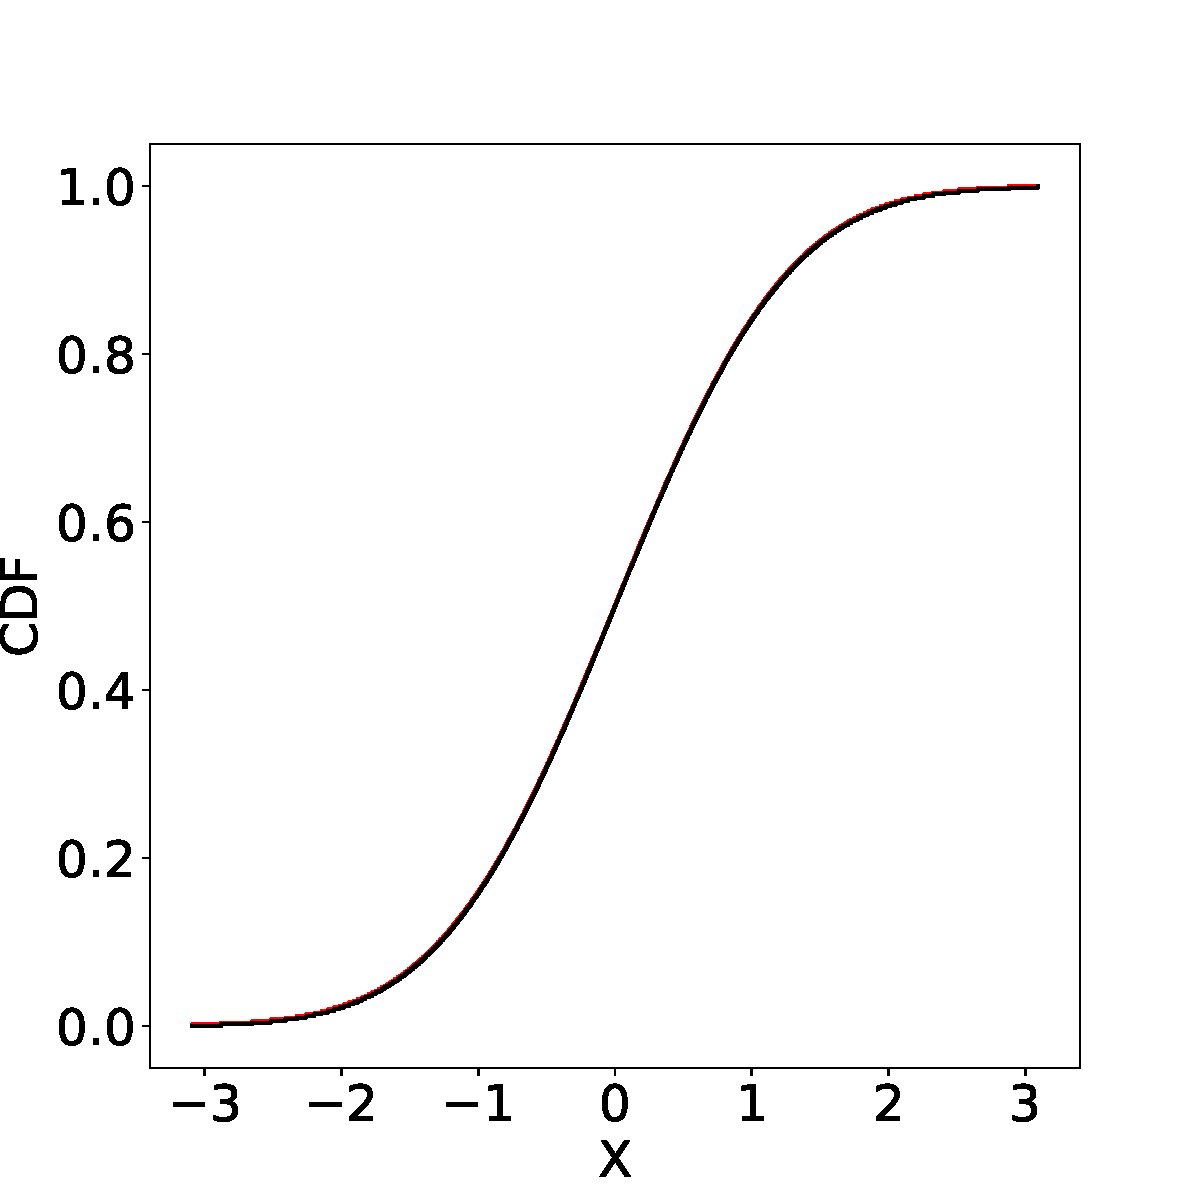
\includegraphics[width=.3\textwidth]{../examples/JuliaCon/fig1/fig1_dist.pdf}\hfill
  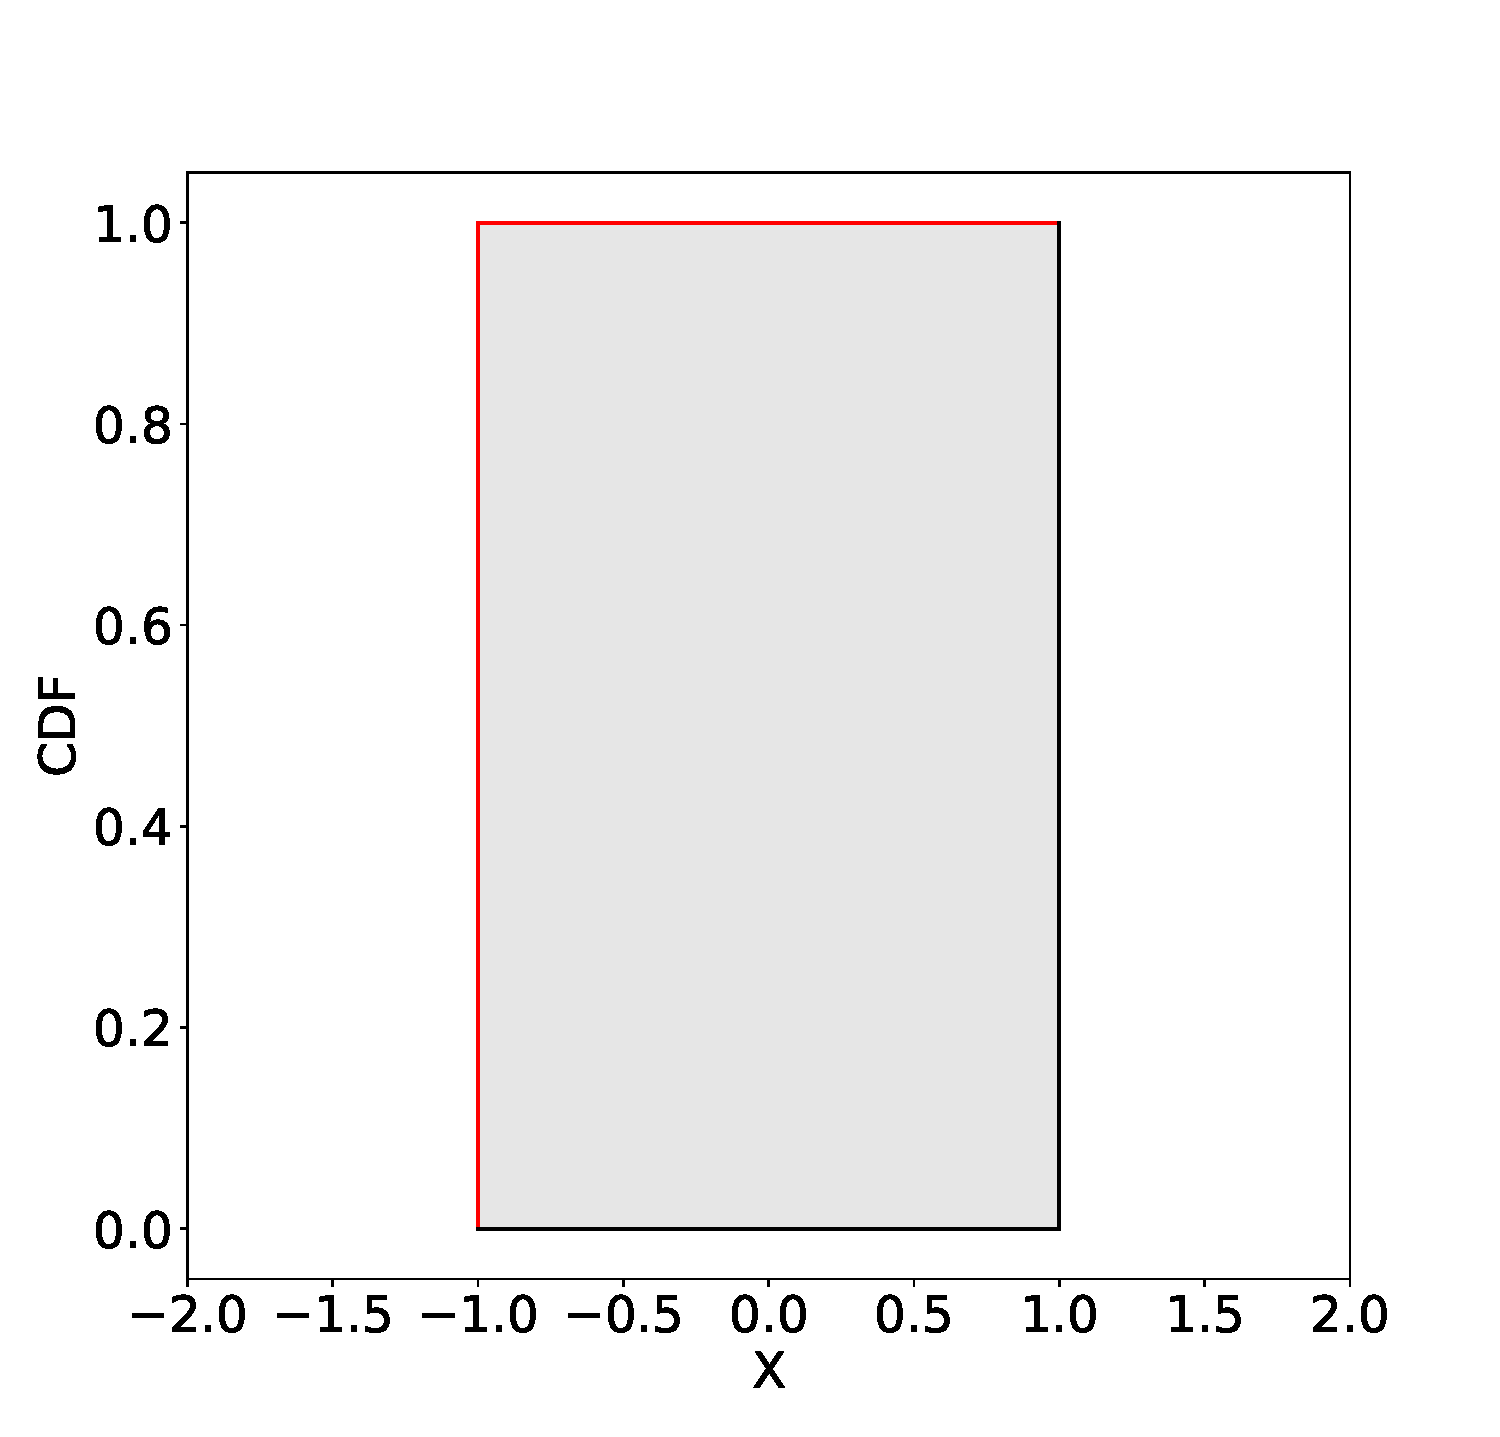
\includegraphics[width=.3\textwidth]{../examples/JuliaCon/fig1/fig1_interval.pdf}\hfill
  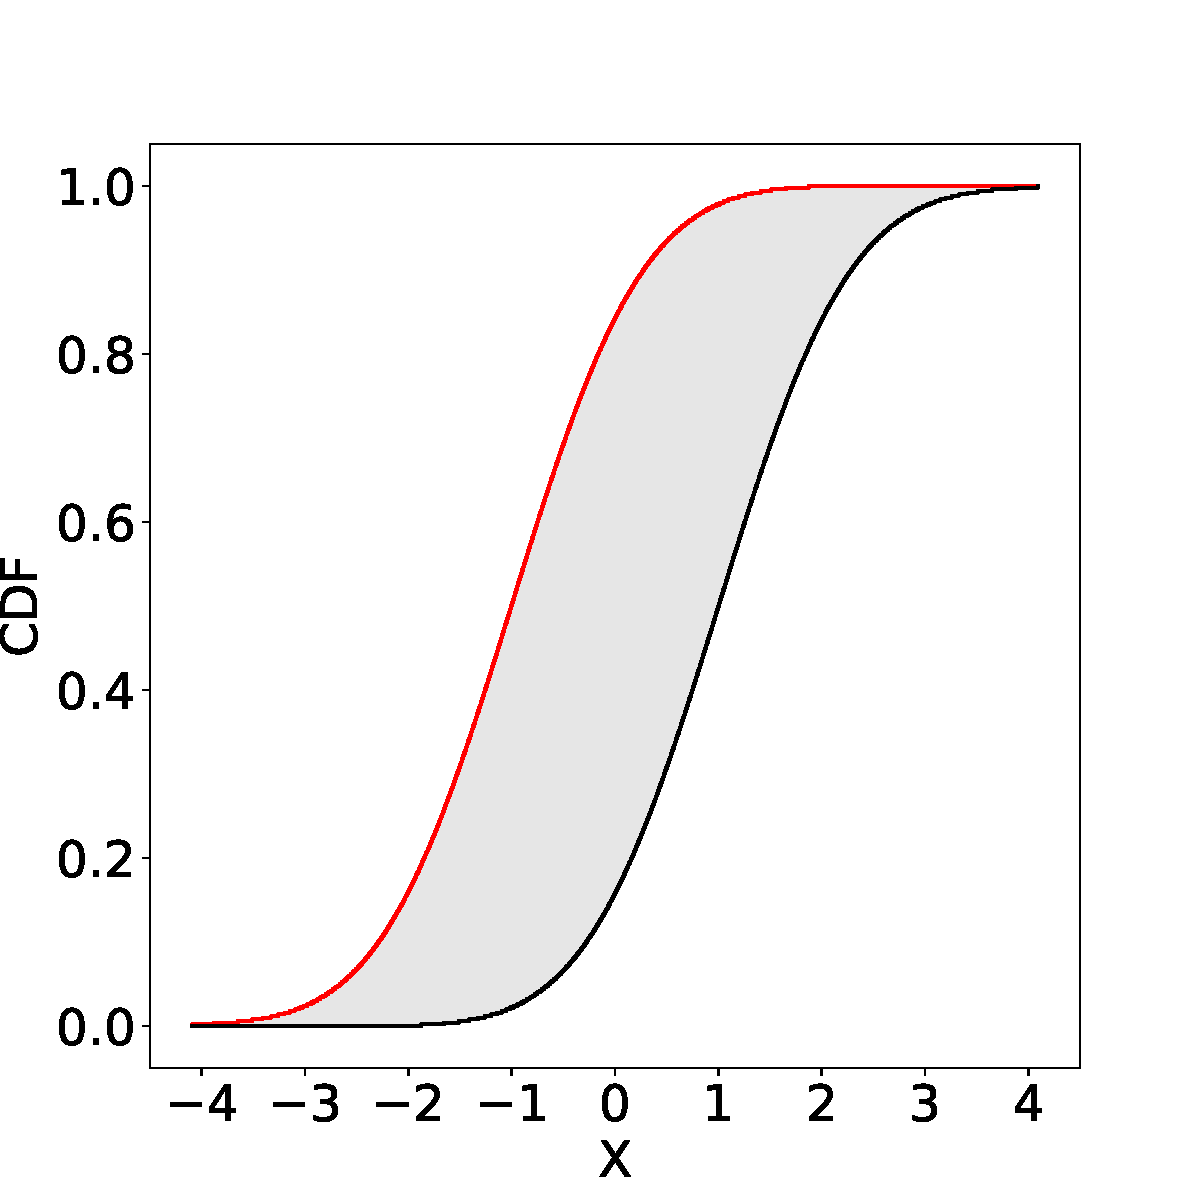
\includegraphics[width=.3\textwidth]{../examples/JuliaCon/fig1/fig1_pbox.pdf}
  
  \caption{A precise distribution, an interval and a probability box}
  \label{fig:figure1}
  
\end{figure*}

\iffalse
\subsection{Automatic uncertainty in a programming language: why Julia?}

The long term goal of probability bounds analysis is to create a fully uncertain programming language, where any computer variable may be represented as an interval, distribution, p-box or other imprecise quantity. Such a framework would allow for uncertain extensions of deterministic functions to be computed in an automatic, rigorous and tight fashion. Those with little knowledge of probability theory can add uncertainty to their computations with minimal effort. Stochastic calculations often require many years of training to implement and interpret correctly, and are usually not rigorous and are famously computationally expensive. \texttt{ProbabilityBoundsAnalysis.jl} provides the type structure for distribution functions and p-boxes which is rigorous, and has many of the base operations required for an uncertain programming language, which are rigorous and computationally effient. In this section we argue why Julia is an ideal target language for such an uncertainty language.


\subsubsection{Multiple dispatch} \hfill \break

Multiple dispatch allows Julia packages with completely different functionalities to work together with minimal effort. One of the great successes of \texttt{IntervalArithmetic.jl} is that it allows for intervals to be propagated through nearly any Julia function, including those from different packages.

\subsubsection{Parametric typing} \hfill \break

Parametric typing allows one to create very generic data types, parametrised on other types. This is 

For example, an uncertain

an interval of type Int64 (\texttt(Interval{Int64})) can be made and destiguised of t

\subsubsection{Metaprogramming} \hfill \break

Blah blah blah 

\subsubsection{Native parallelisation} \hfill \break

Blah blah blah 

%, and discuss some of the remaining theoretical tasks required to make such a goal a reality. 
\fi
\section{Probability Boxes}
\label{sec:pboxes}

A real-valued random variable is characterised by its distribution function $F$, which is a monotonically increasing function from the real numbers onto the interval $[0, 1]$ such that the value of the function at negative infinity is zero and the value of the function at positive infinity is one.  A p-box consists of a pair of such functions that are used to circumscribe an imprecisely known distribution function $F$. The p-box, in its simplest form consisting of the pair of bounding functions, identifies a set of probability distributions that lie entirely within these bounds. Additional information about the random variable may be available, such as bounds on its mean and variance and its distribution family, which may be used to further restrict the set of distributions. A p-box is thus defined by the following three constraints: (1) two bounding cumulative distribution functions (cdf), (2) interval bounds on the mean and variance, and (3) a collection of distribution families:

\begin{enumerate}
  \item $\begin{aligned}[t]
    \underline{F}(x) \leq F(x) \leq \overline{F}(x) \\%&&&& \text{(Bounds on the cdf)} \\
  \end{aligned}$
  \item $\begin{aligned}[t]
    \mu &\in [\underline{ \mu }, \overline{ \mu }]  \\%&&&& \text{(bounds on mean and variance)}\\
    \sigma^2 &\in [\underline{\sigma}^2 , \overline{\sigma}^2]
  \end{aligned}$
  \item $\begin{aligned}[t]
      F \in \bold{F} \\%&&&&&&& \text{(distribution family)} \\
  \end{aligned}$
  \end{enumerate}

\noindent That is, a random variable is a member of a p-box if its cdf $F$ falls within the cdf bounds of the p-box $F(x) \in [\underline{F}(x), \overline{F}(x)]$ for all $x$, its moments are inside the interval moments of the p-box, and it belongs to a family of distribution functions (e.g. normal, uniform) considered by the p-box. Some of the constraints may be missing. For example, if the distribution family is unknown then the set is defined solely from the cdf and moment bounds. Such p-boxes are sometimes called non-parametric, since its members do not belong to any particular class of distribution. Some constraints may also be inferred from others. For example, the interval moments may be bounded from the cdf bounds, and cdf may be bounded from moment information (explored further in section \ref{section:Moments}). Figure\footnote{Scripts for all figures can be found in /examples/JuliaCon.} \ref{fig:figure1} shows an example of a distribution function, interval and a p-box. The grey shaded region in the interval and p-box bounds an infinite collection of probability distributions.


\begin{figure*}[htp]

  \centering
  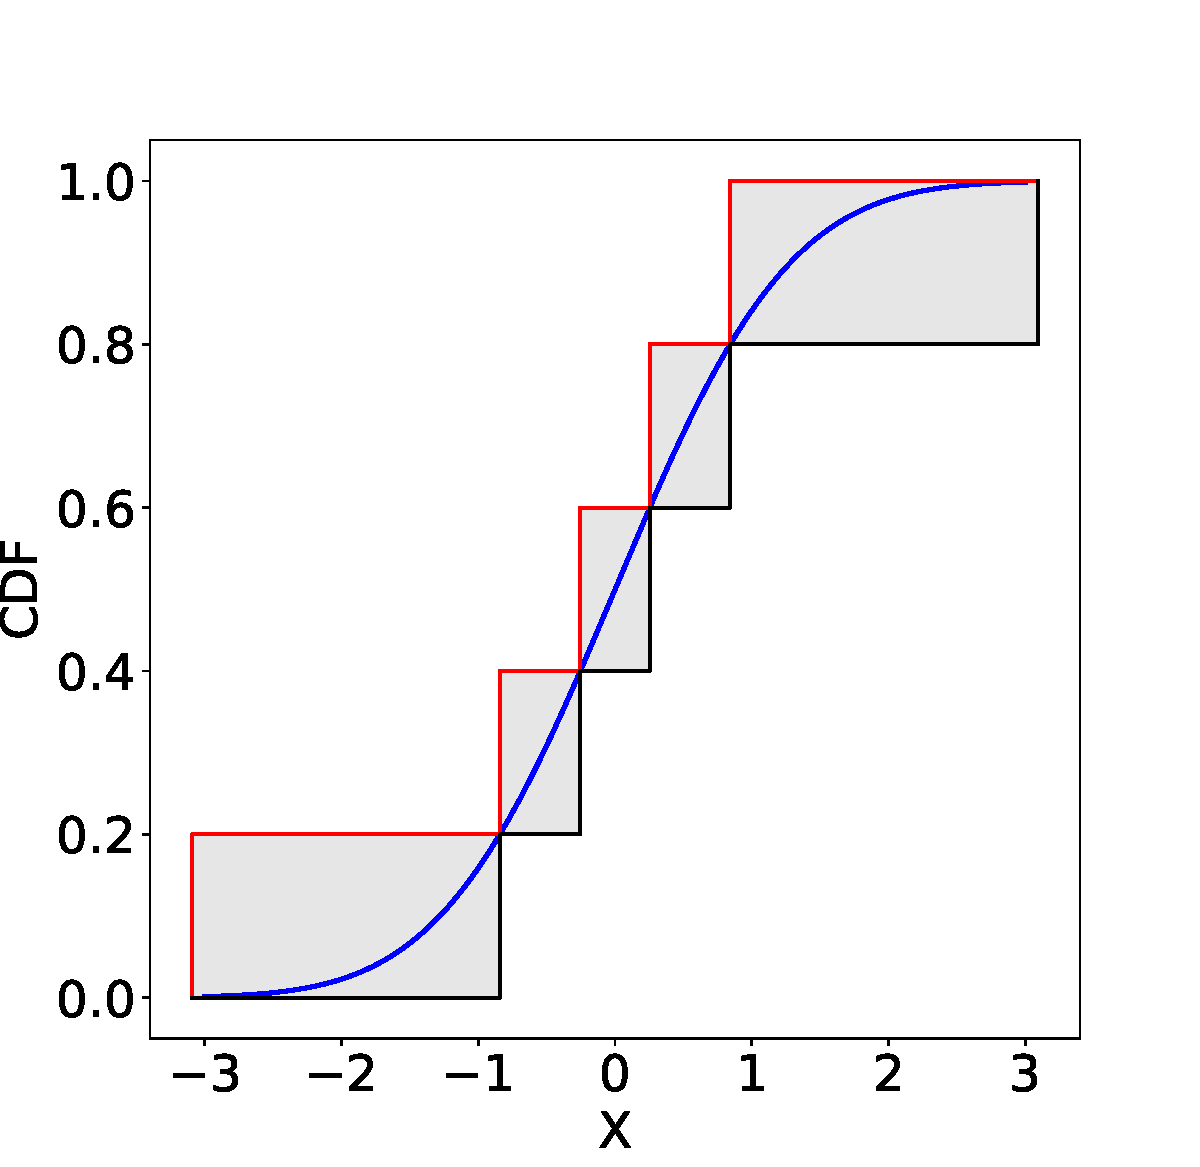
\includegraphics[width=.3\textwidth]{../examples/JuliaCon/fig2/fig2_pbox2.pdf}\hfill
  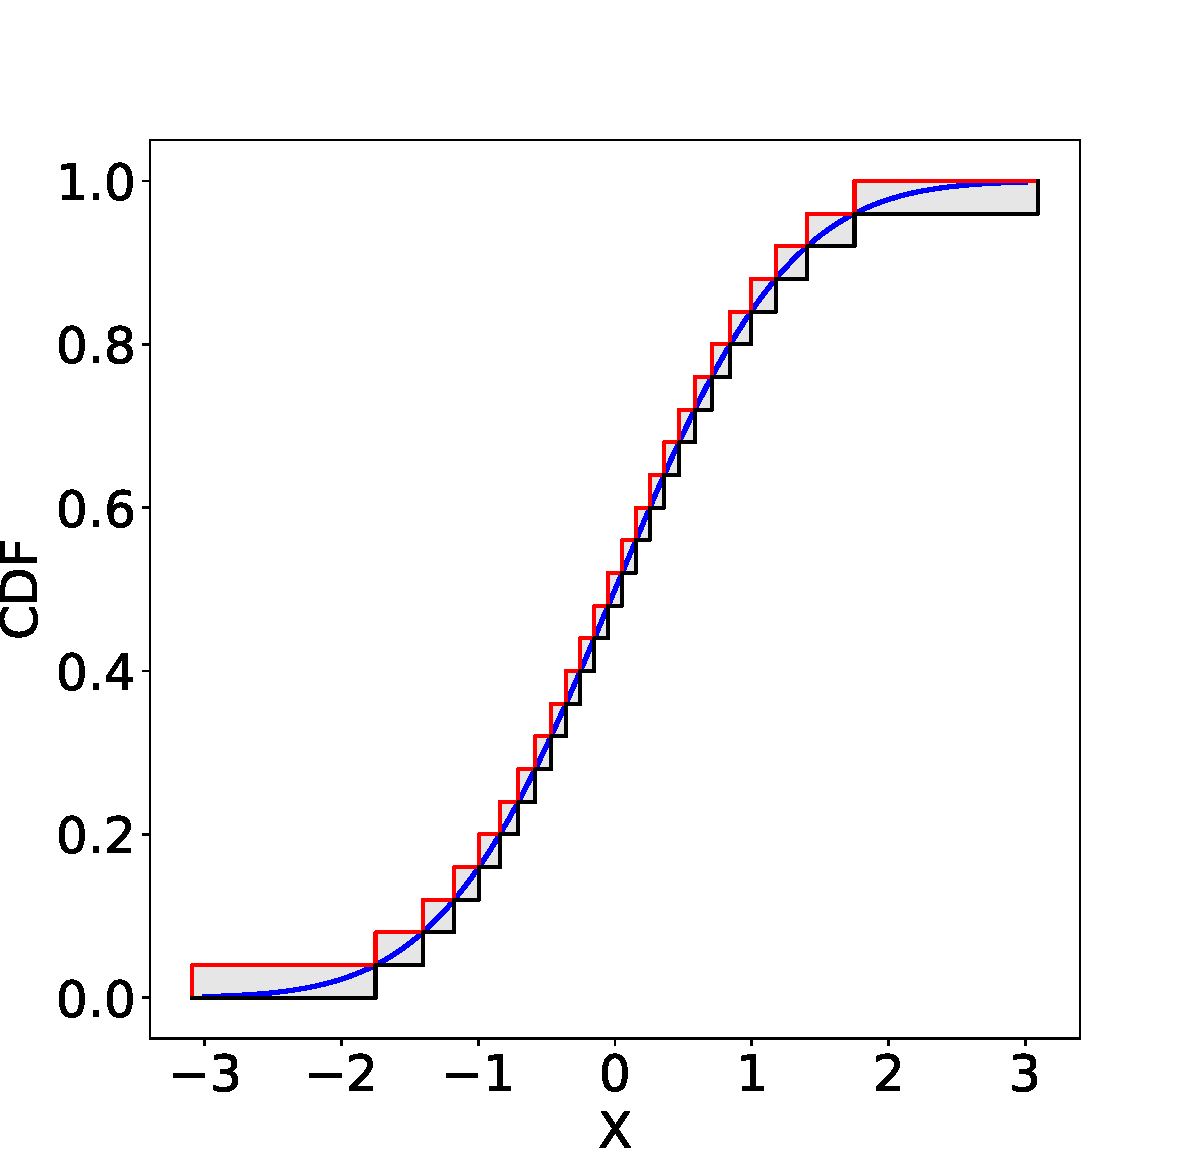
\includegraphics[width=.3\textwidth]{../examples/JuliaCon/fig2/fig2_pbox1.pdf}\hfill
  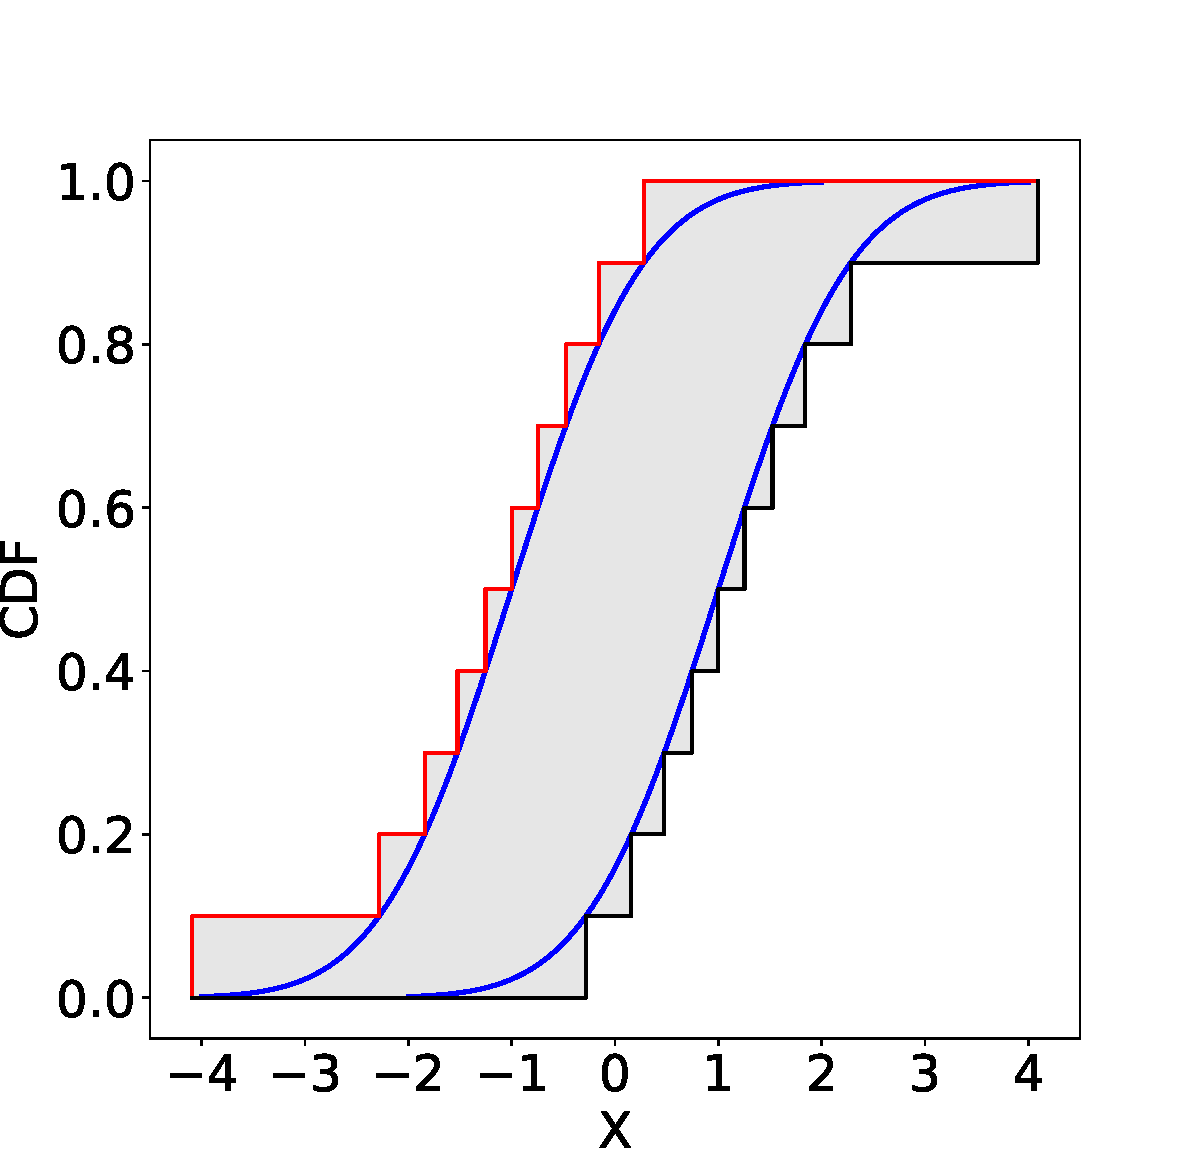
\includegraphics[width=.3\textwidth]{../examples/JuliaCon/fig2/fig2_pbox3.pdf}
  
  \caption{Various outer representations of distribution functions, left $4$ steps and centre $25$ steps, and a p-box (right) with 10 steps}
  \label{fig:figure2}
  
\end{figure*}


Real-valued statistics and features of distributions typically become intervals for p-boxes. The cdf of a p-box is: 

\begin{equation*}
  [\underline{F}(x), \overline{F}(x)] .
\end{equation*}

\noindent A sample realisation of the p-box may be drawn using the inverses of the bounding cdfs: 

\begin{equation*}
  [\overline{F}^{-1}(\alpha), \underline{F}^{-1}(\alpha)]
\end{equation*}

\noindent where $\alpha \sim U(0,1)$ is a sample from a uniform distribution. The probability measure,  a function which returns the probability that the random variable is in some set, on some interval $U = [a, b]$ is bounded as follows:

\begin{align*}
  \underline{\mathbb{P}}(U) &= \text{max}(0, \underline{F}(b) - \overline{F}(a)) \\ 
  \overline{\mathbb{P}}(U)  &= \overline{F}(b) - \underline{F}(a) ,
\end{align*}

where the max operator is required when $\underline{F}(b) < \overline{F}(a)$. Note the same can nearly be achieved by using the precise formula for the probability measure, $\mathbb{P}(U) = F(b)- F(a)$, and using interval arithmetic.


P-boxes generalise precise distributions and intervals in the following way. A distribution is a p-box with a precise cdf and moments, i.e. when: 

\begin{align*}
  \underline{F}(x) &= \overline{F}(x), \\ 
  \underline{\mu}  &= \overline{\mu}, \\ 
  \underline{\sigma}^2 &= \overline{\sigma}^2 .
\end{align*}

\noindent An interval $[a,b]$ is a p-box whose bounds are step functions: 

\begin{align*}
    \underline{F}(x) &= \epsilon_{b}(x) ,\\
    \overline{F}(x) &= \epsilon_{a}(x) ,
\end{align*}

\noindent where $\epsilon_k$ is: 

\begin{equation*}
   \epsilon_k(x) = \begin{cases} 0 &\text{when } x < k \\ 1 &\text{when } x \geq k \end{cases}
\end{equation*}

Moreover, theoretical bounds on the mean and variance of an interval can be found \cite{ferson2002ramas}:

\begin{align*}
  \mu &\in [a, b] \\
  \sigma^2 &\in [0, (b - a)^{2/4}]
\end{align*}

That is, it is not possible to find a distribution whose range is in $[a, b]$ and whose variance is greater than $(b-a)^{2/4}$. The lower bound on the variance is zero, since scalars are also included in the interval. Under this definition of an interval, a random sample will always be the interval $[a, b]$, the cdf returns 0 when $x < a$, the interval $[0,1]$ when $a <= x < b$, and $1$ when $b <= x$. Further, the probability measure of the interval $X = [a, b]$ will be: 

\begin{equation*}
  \mathbb{P}_{X}(U) = \begin{cases}
    0 & \text{when } U \cap [a,b] = \emptyset \\
    1 & \text{when } [a,b] \subseteq U  \\
    [0, 1] & \text{otherwise }\\
  \end{cases}
\end{equation*}

\noindent That is, if the set $U$ does not intersect the interval $X$, $\mathbb{P}_{X}=0$, i.e. $U$ certainly does not contain any of the random variables. If $X$ is fully contained in $U$, $\mathbb{P}_{X}=1$, i.e. $U$ certainly contains all of the random variables. And finally if $U$ intersects (but does not contain) $X$, the probability measure is the vacuous probability interval $\mathbb{P}_{X} = [0, 1]$, i.e. we are completely uncertain about the containment. Note that the $P_{X} = \{0, 1, [0,1]\}$ is due to the interval bounds being step functions. Generally p-boxes may yield other probability intervals.

\subsection{Outer representations of p-boxes}
\label{sec:outer_approx}

An important feature of probability bounds analysis is how distribution functions and p-boxes are represented. Generally, analytical solutions for cdfs are not readily available, for example the normal distribution's cdf can only be found by integrating the probability density, usually with quadrature. However, even if the functions were available analytically, when the variables are used in an arithmetic operation the output distribution will not necessarily belong to the same family. Therefore, we require a representation of these continuous functions which is not dependent on the distribution family (for example as used in polynomial chaos expansion), and ideally is robust in the sense that it can produce an interval error for the numerical representation. Such a representation of a probability is sometimes called an "outer approximation", in the same fashion an interval is an outer approximation of a floating point number. Such outer approximations contract to the exact value or function as more computational resources are used.

We follow the representation first introduced by Williamson and Downs \cite{williamson1990probabilistic}, where a discrete upper and lower approximations of distribution functions are constructed using the inverse cdfs. Note that when considering inverse cdfs $\underline{F}^{-1}(p) \geq F^{-1}(p) \geq \overline{F}^{-1}(p)$, for $p \in [0,1]$. An outer approximation using two finite vectors\footnote{We begin vector indexing with $1$ as is done in the Julia language.} $u$ and $d$ of length $N$ is constructed by evaluating the inverse cdfs for uniformly spaced probability levels $p_{i} = \frac{i-1}{N}$ for $i = 1, ... , N+1$, e.g. $p_{i} = [0, 0.25, 0.5, 0.75, 1]$ for $N = 4$. The vectors $u$ and $d$ are defined as follows:

\begin{align*}
  u[i] &= \overline{F}^{-1}(p_{i}) \\ 
  d[i] &= \underline{F}^{-1}(p_{i+1}) & \text{for } i = 1, ..., N
\end{align*}



\begin{figure*}[htp]

  \centering
  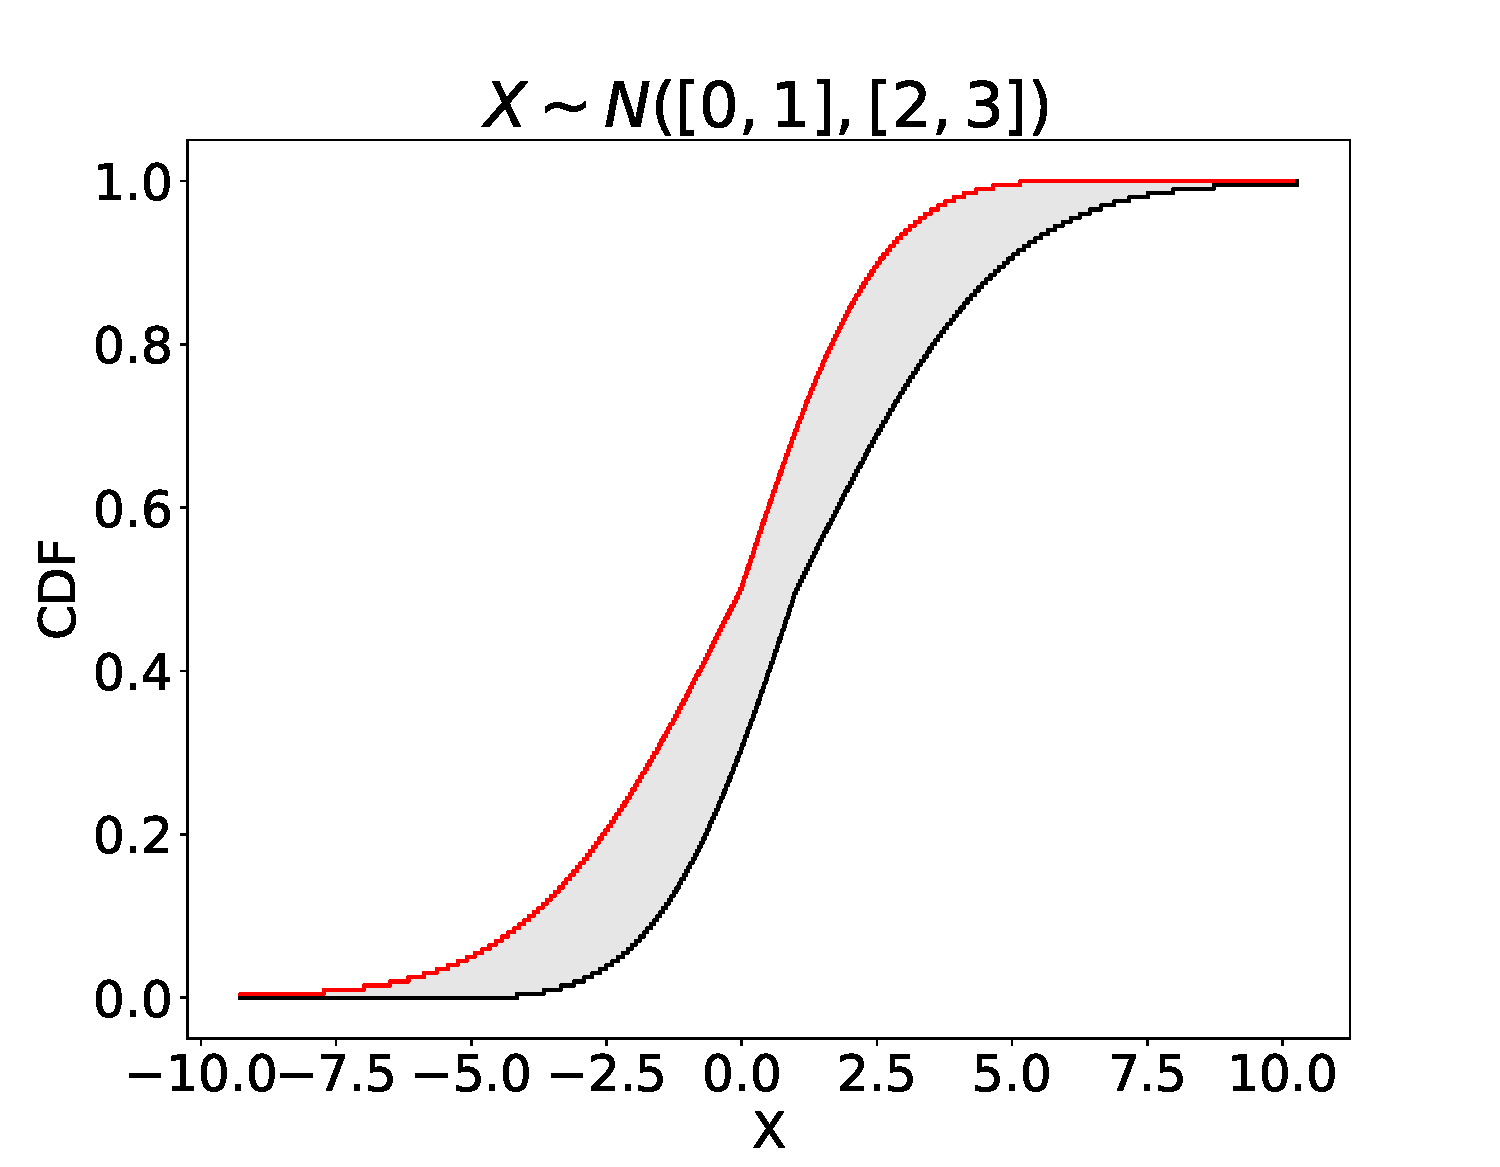
\includegraphics[width=.25\textwidth]{../examples/JuliaCon/fig3/normal.pdf}\hfill
  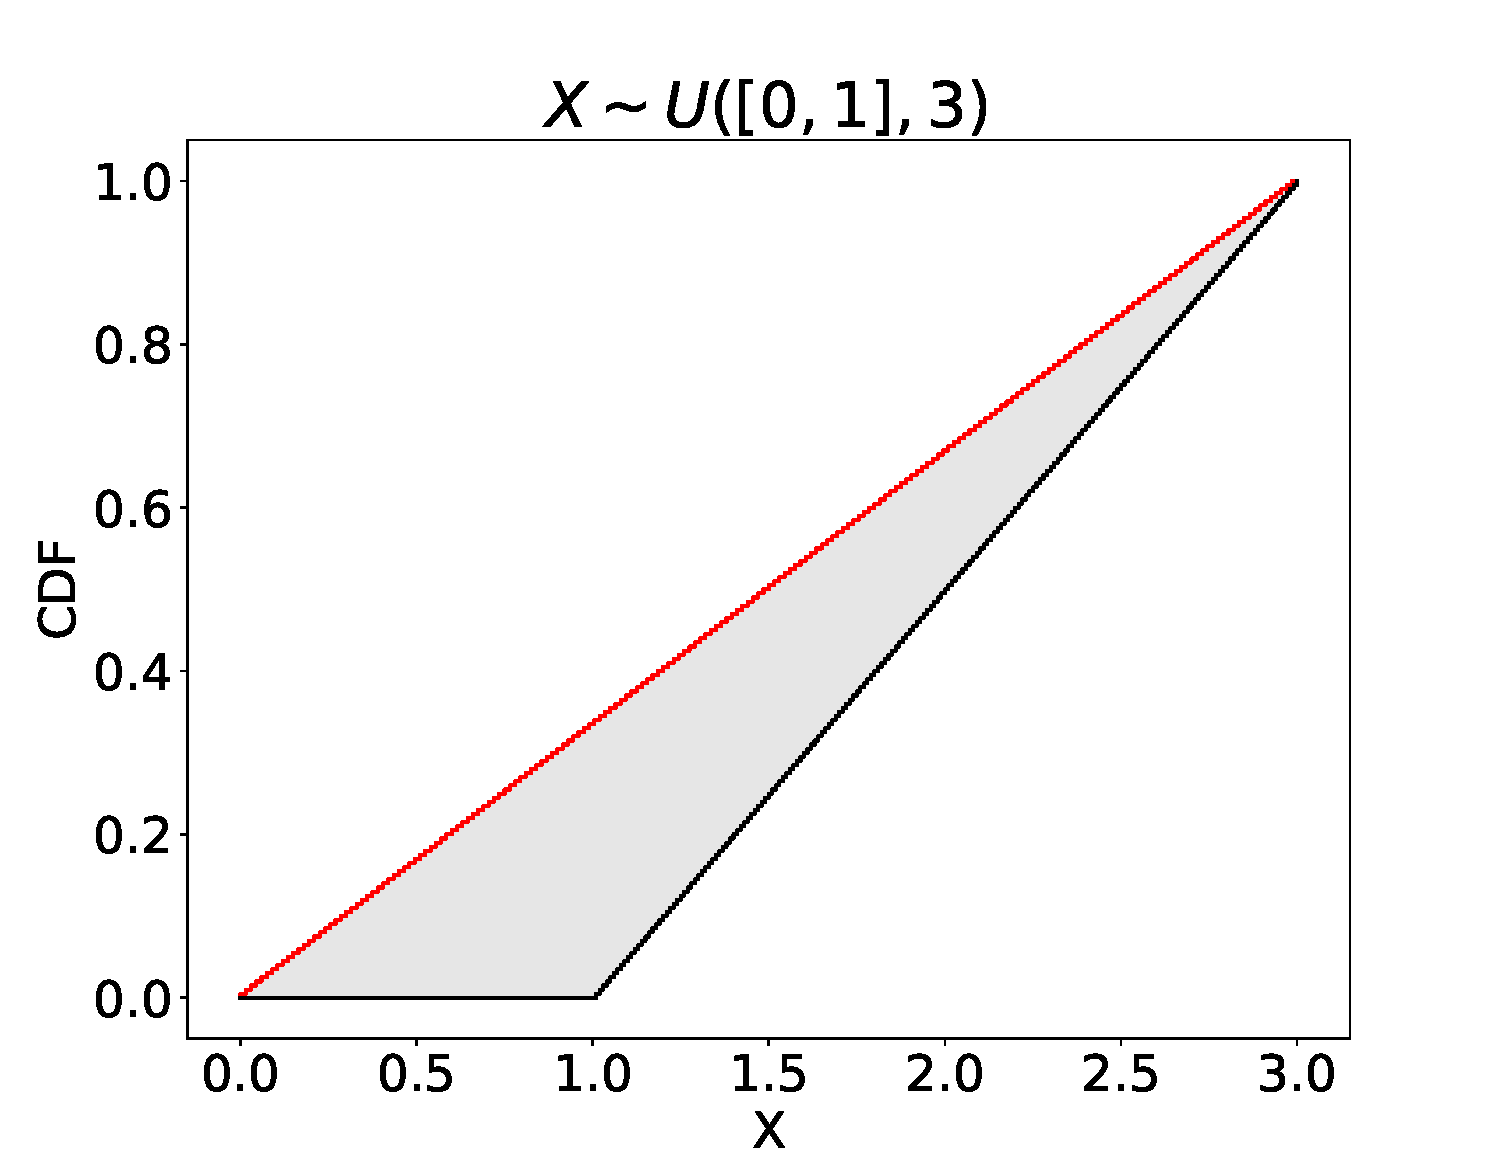
\includegraphics[width=.25\textwidth]{../examples/JuliaCon/fig3/uniform.pdf}\hfill
  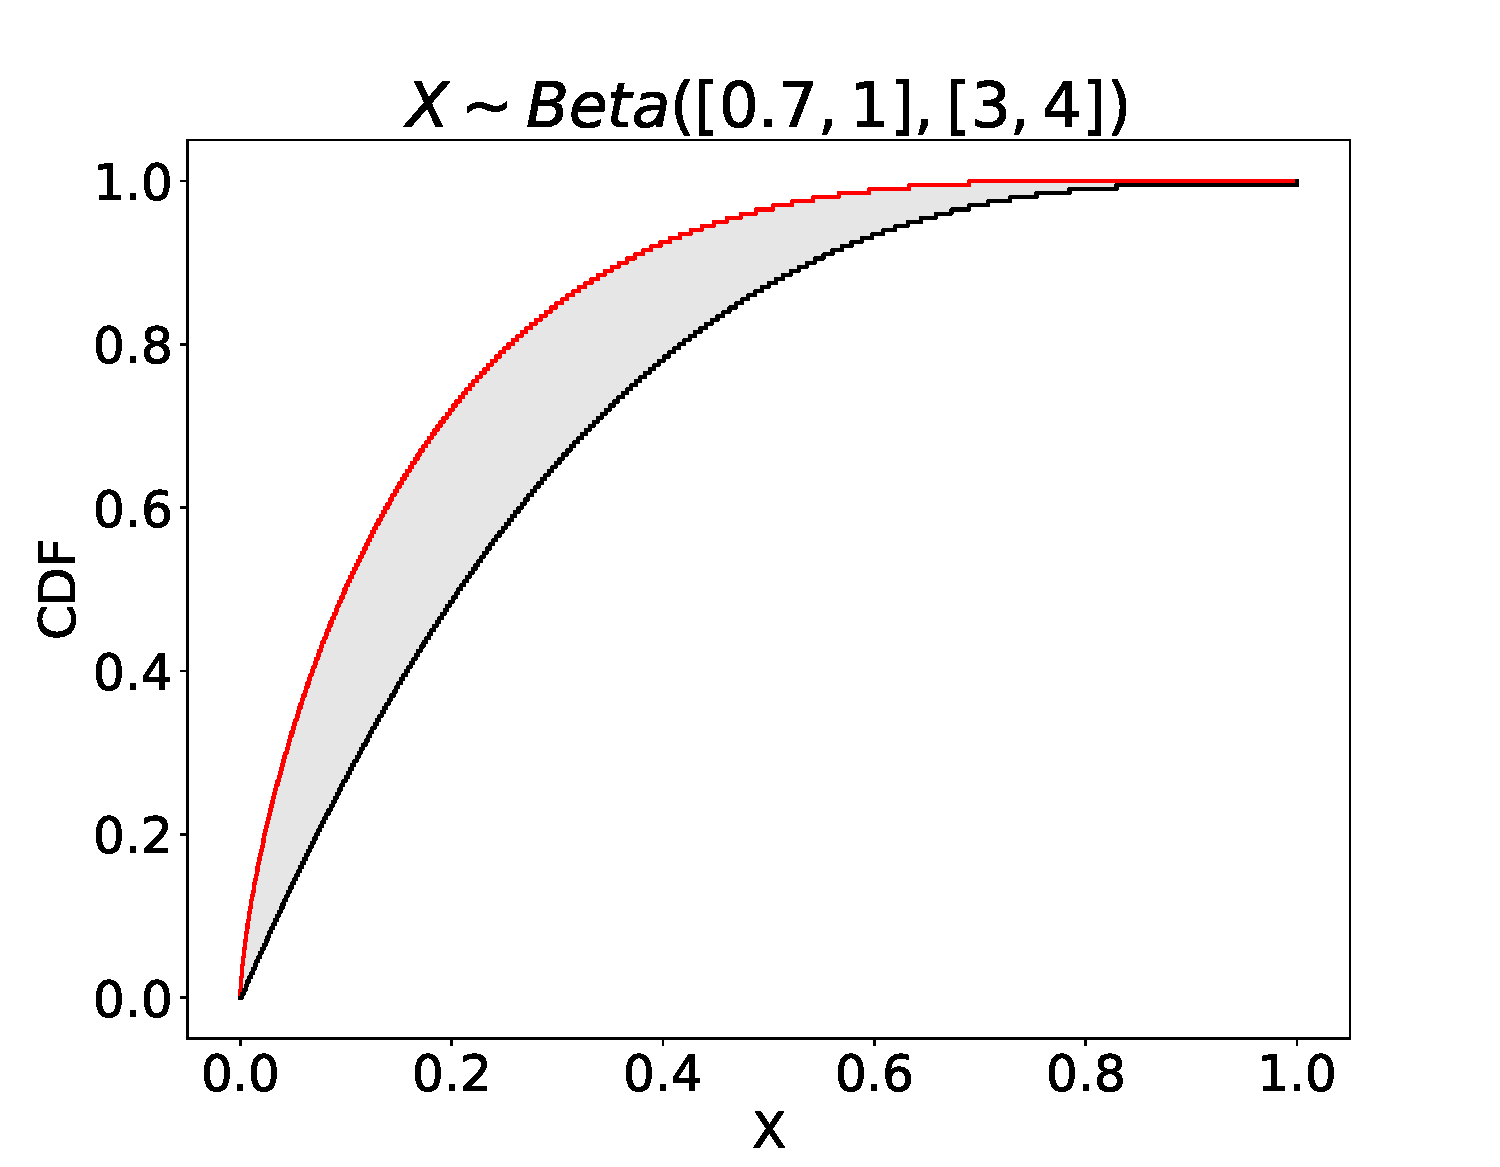
\includegraphics[width=.25\textwidth]{../examples/JuliaCon/fig3/beta.pdf}\hfill
  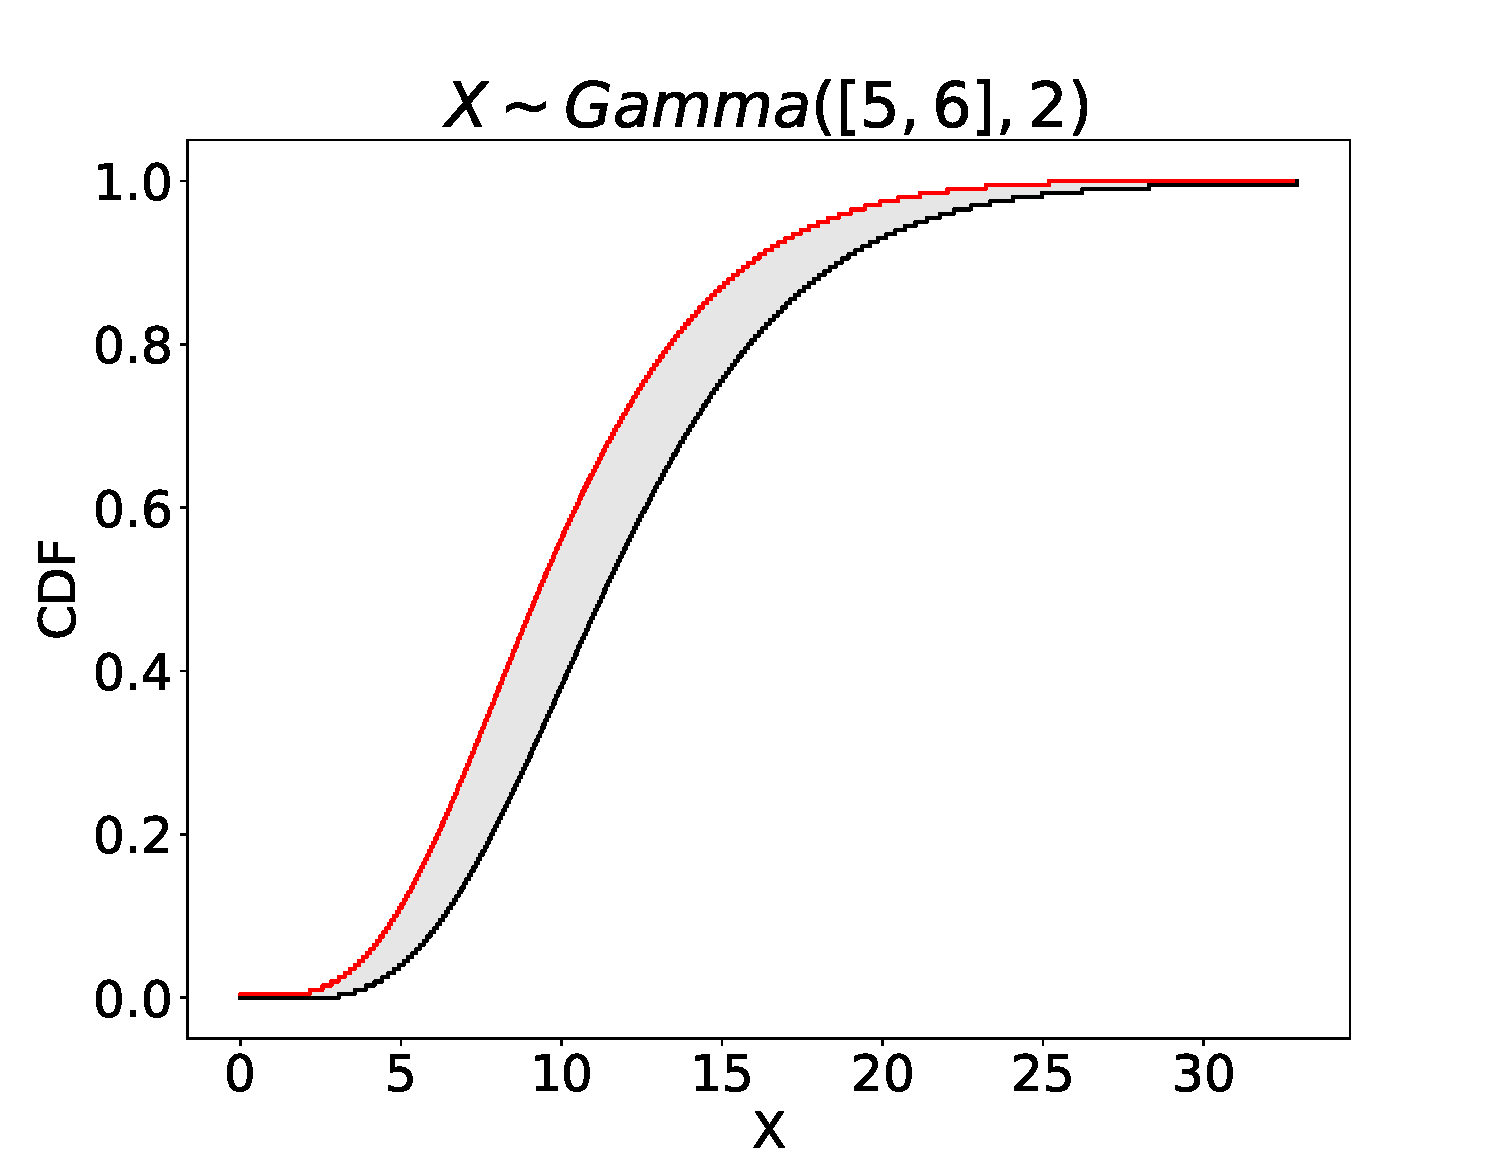
\includegraphics[width=.25\textwidth]{../examples/JuliaCon/fig3/gamma.pdf}
  

  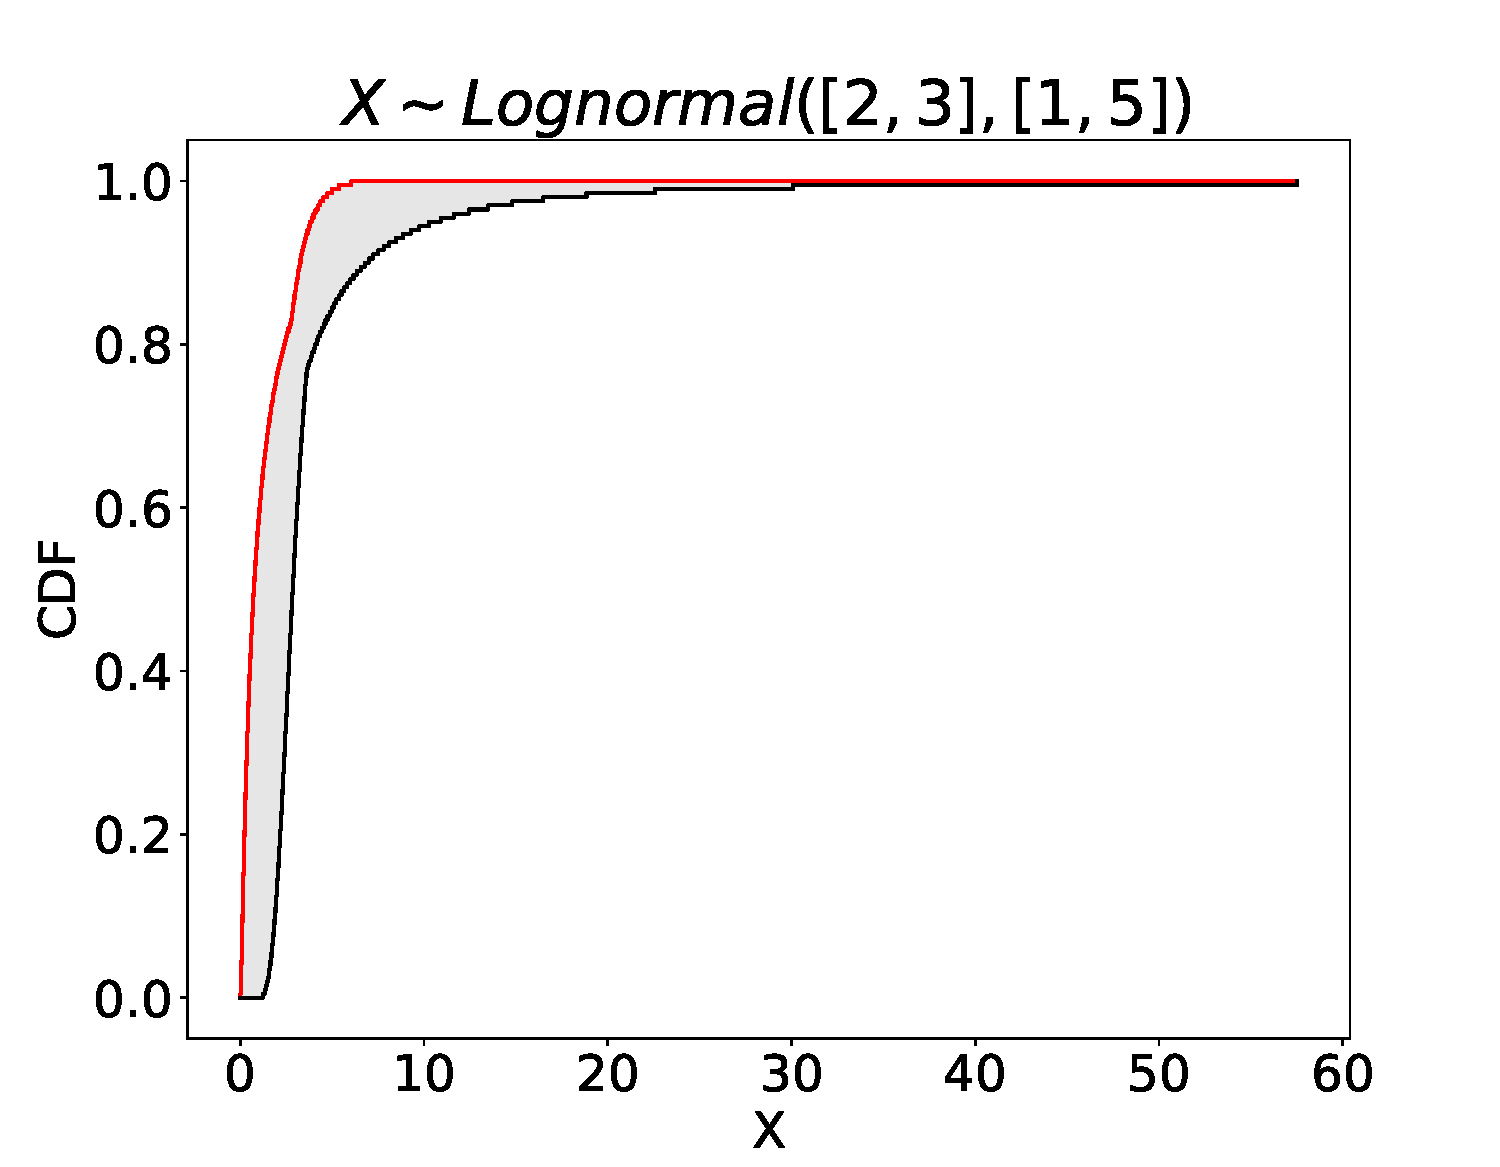
\includegraphics[width=.25\textwidth]{../examples/JuliaCon/fig3/lognormal.pdf}\hfill
  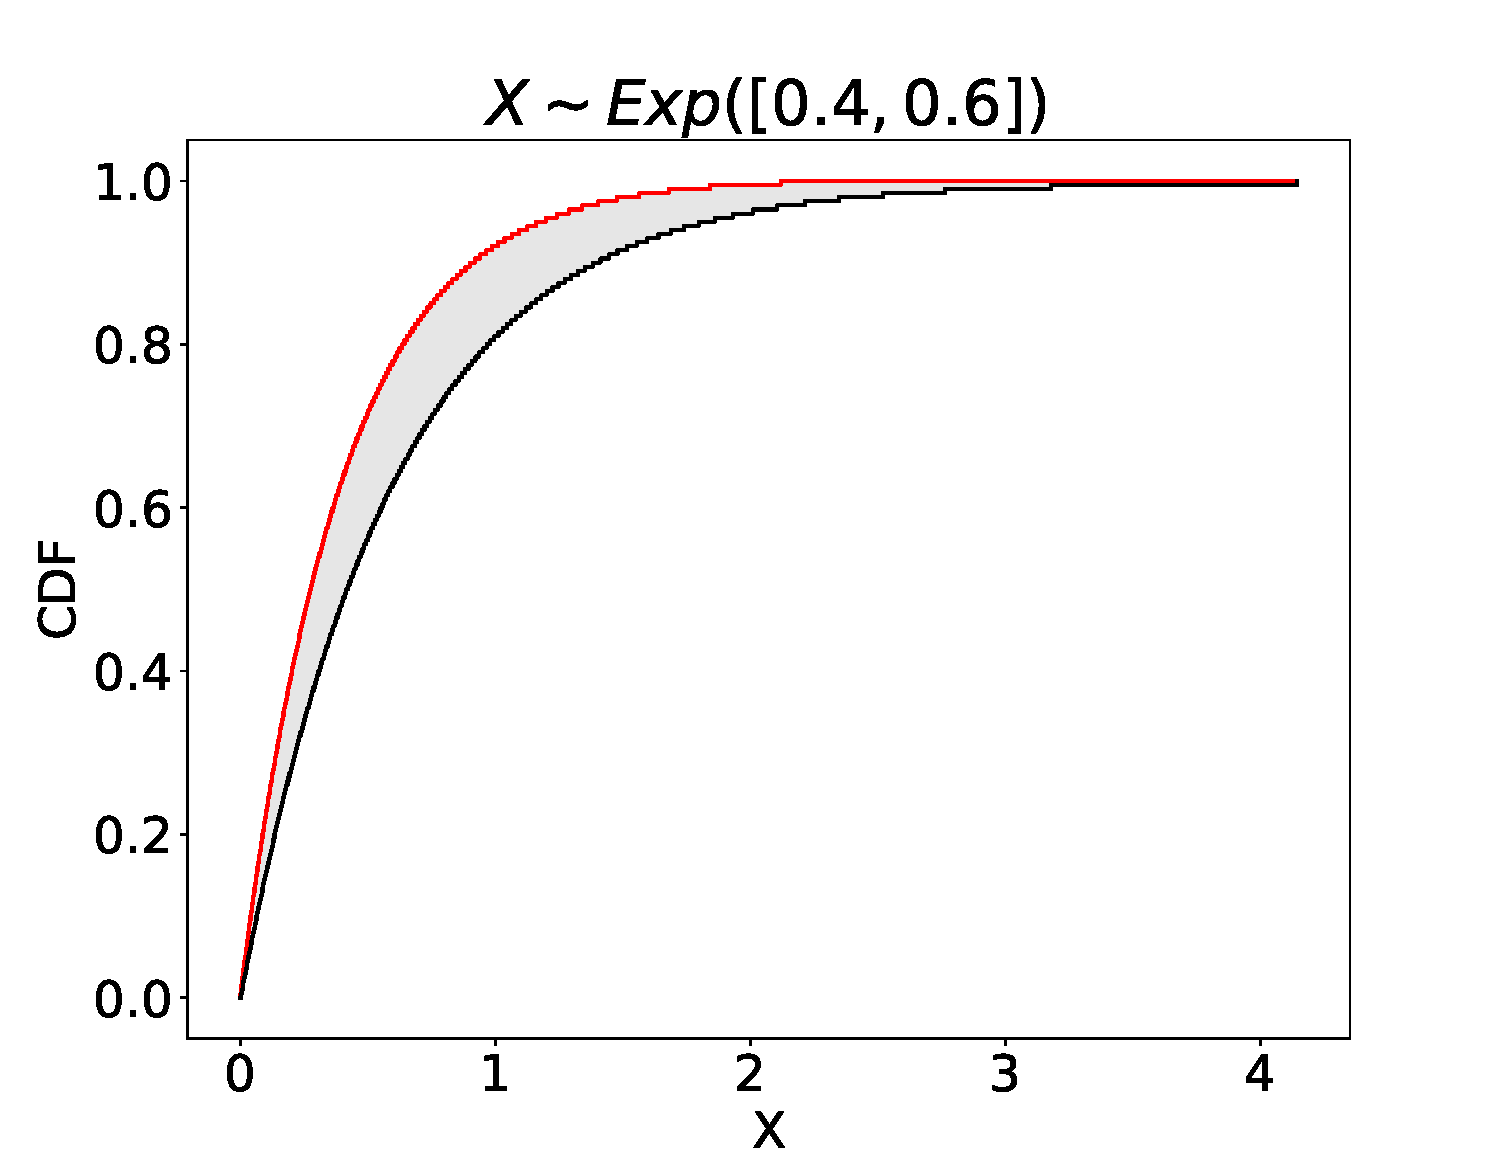
\includegraphics[width=.25\textwidth]{../examples/JuliaCon/fig3/exponential.pdf}\hfill
  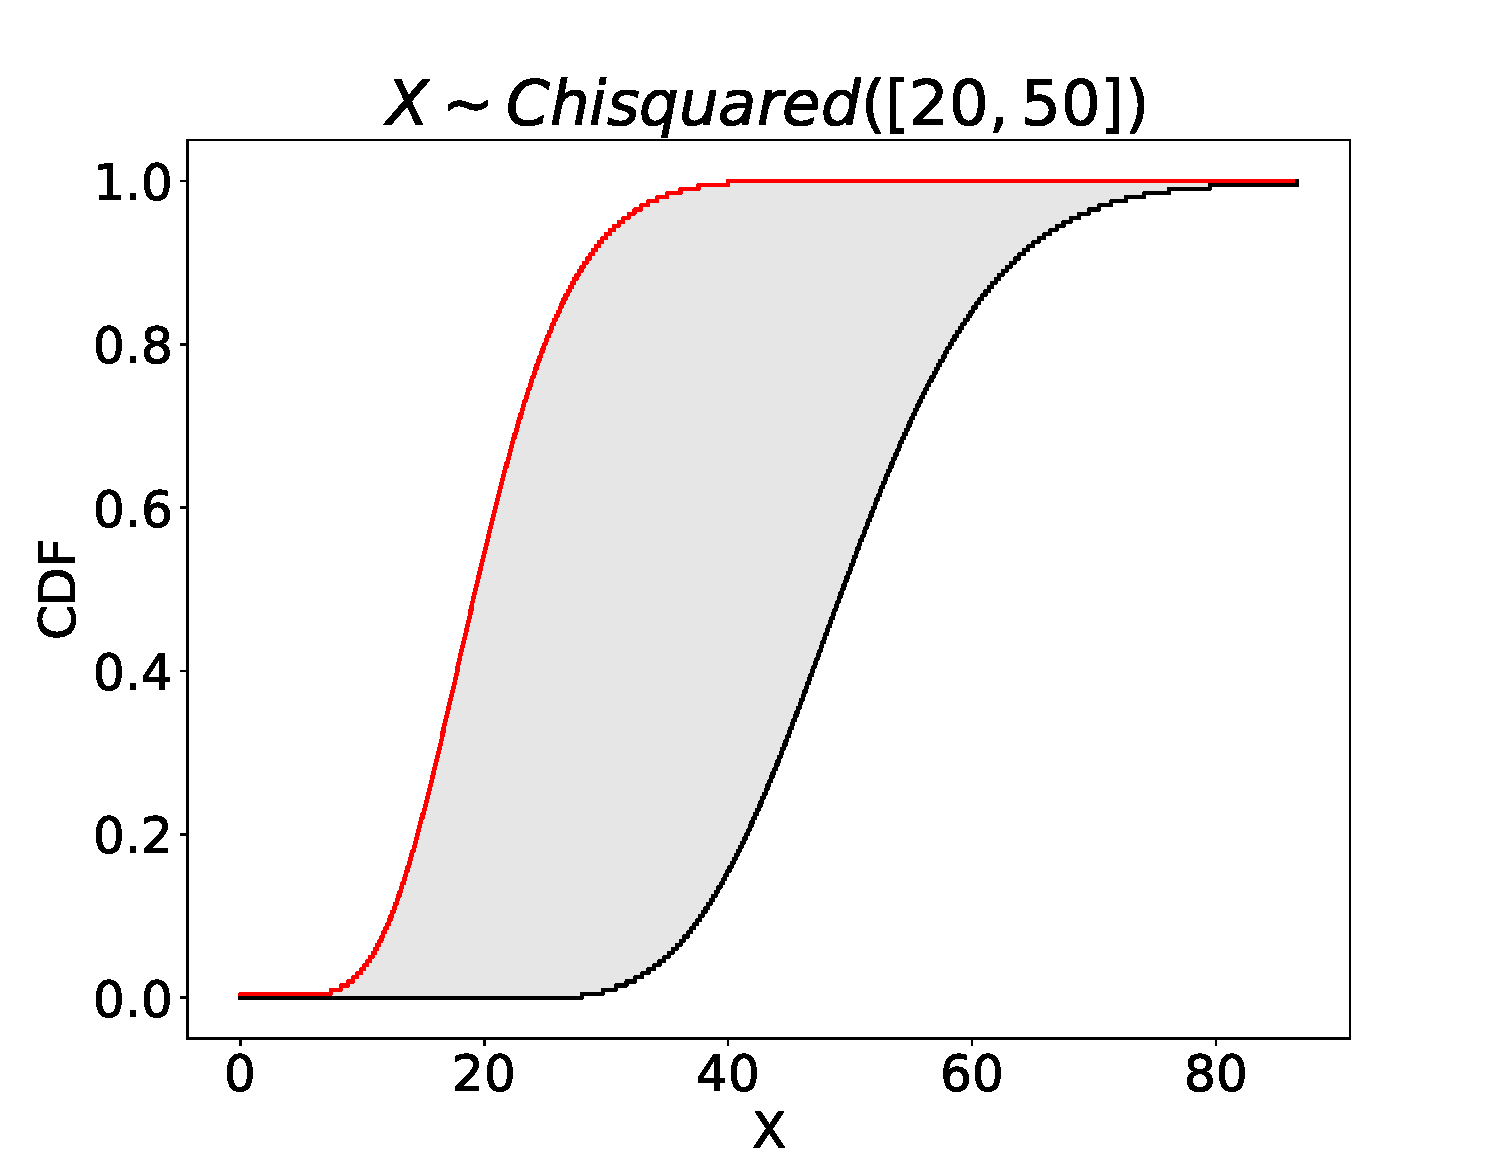
\includegraphics[width=.25\textwidth]{../examples/JuliaCon/fig3/chisquared.pdf}\hfill
  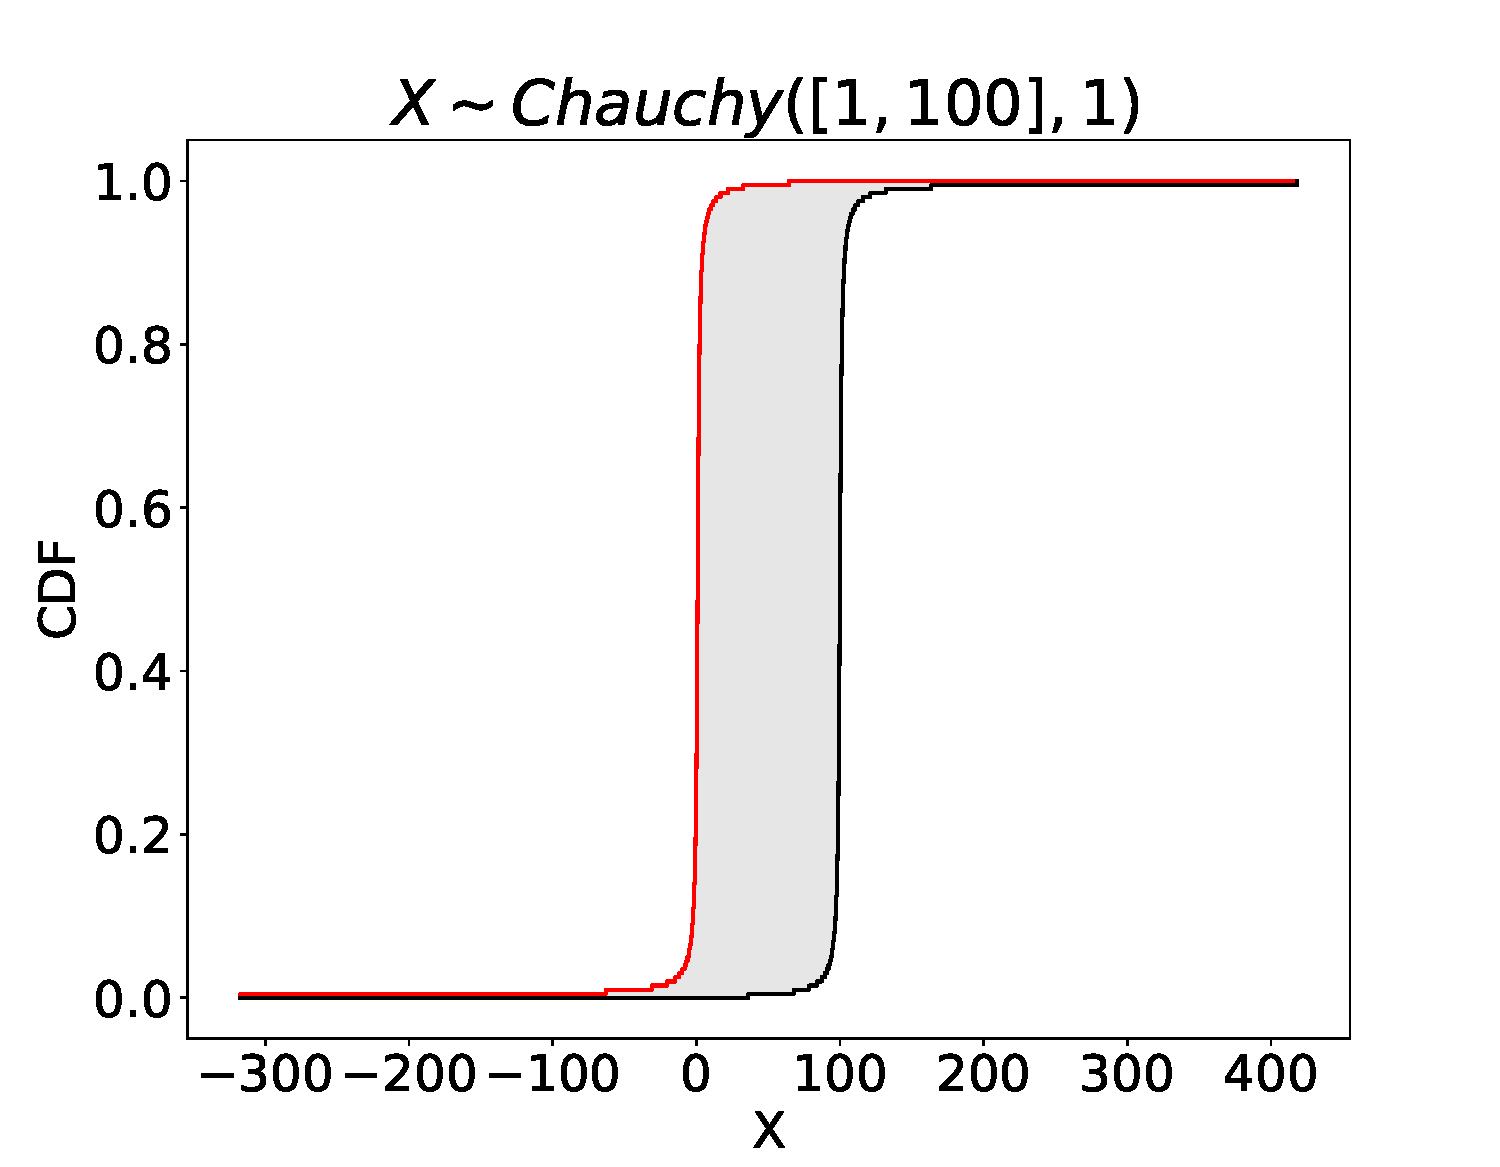
\includegraphics[width=.25\textwidth]{../examples/JuliaCon/fig3/cauchy.pdf}
  

  \caption{Various parametrically constructed p-boxes with interval parameters}
  \label{fig:figure3}
  
\end{figure*}


The vectors $u$ and $d$ are a collection of "real" or "physical" evaluations of a the random variable $X$, as opposed to cdf evaluations. Although the probability levels $p$ are uniformly spaced, $u$ and $d$ are generally not. The vectors $u$ and $d$ can then serve as bounds on the monotonic functions $\overline{F}^{-1}$ and $\underline{F}^{-1}$:

\begin{align*}
  u[i] &\leq \overline{F}^{-1}(p) & p_{i} \in [p_{i}, p_{i+1} )\\ 
  d[i] &\geq \underline{F}^{-1}(p) & p_{i} \in (p_{i}, p_{i+1}]
\end{align*}

That is, in the region $[p_{i}, p_{i+1})$, $u[i]$ is a lower bound on $\overline{F}^{-1}$ and $d[i]$ is an upper bound on $\underline{F}^{-1}$ in $(p_{i}, p_{i+1}]$. In the case that the p-box characterises a precise distribution and $\overline{F}^{-1}(p) = \underline{F}^{-1}(p)$ gives:  $u[i+1] = d[i]$. Figure \ref{fig:figure2} shows examples of a distribution and a p-box with various outer representations.

A minimal\footnote{The code for the minimal structure can be found in examples/minimal.} p-box structure is as follows:

\begin{lstlisting}[language = Julia]
  using IntervalArithmetic

  struct pbox{T <: Real}
    u :: Vector{T}    # left discrete inverse
    d :: Vector{T}    # right discrete inverse
    m :: Interval{T}  # interval mean
    v :: Interval{T}  # interval variance
    shape :: String   # shape
  end
\end{lstlisting}

\noindent where the vectors $u$ and $d$ are the "up" and "down", or the "left" and "right", edges of the p-box\footnote{There can be confusion since $\overline{F}$ is the upper bound on the cdf, but $\overline{F}^{-1}$ is the lower bound on the random variable, i.e. the left edge of the p-box. We therefore $\overline{F}$ the "up" or "left" edge, and $\underline{F}$ the "down" or the "right" edge.}. The intervals $m$ and $v$ are the interval moments, and the $shape$ is a string containing any distribution family information. An example of a normal distribution constructor is as follows:

\begin{lstlisting}[language = Julia]
  using Distributions
  const steps = 200

  function normal(m :: Interval, std :: Interval)

    ps = range(0, 1, length = steps+1)

    b1 = quantile.(Normal(m.lo, std.lo), ps)
    b2 = quantile.(Normal(m.lo, std.hi), ps)
    b3 = quantile.(Normal(m.lo, std.hi), ps)
    b4 = quantile.(Normal(m.hi, std.hi), ps)

    u = min.(b1, b2, b3, b4)[1:end-1]
    d = max.(b1, b2, b3, b4)[2:end]

    return pbox(u, d, m, std^2, "normal")
  end
\end{lstlisting}

\iffalse
\begin{lstlisting}[language = Julia]
  using Distributions
  const steps = 200

  function normal(m :: Interval, std :: Interval)

    ps = range(0, 1, length = steps+1)

    ps_u = ps[1:end-1]
    ps_d = ps[2:end]

    u1 = quantile.(Normal(m.lo, std.lo), ps_u)
    u2 = quantile.(Normal(m.lo, std.hi), ps_u)
    u3 = quantile.(Normal(m.lo, std.hi), ps_u)
    u4 = quantile.(Normal(m.hi, std.hi), ps_u)

    d1 = quantile.(Normal(m.lo, std.lo), ps_d)
    d2 = quantile.(Normal(m.lo, std.hi), ps_d)
    d3 = quantile.(Normal(m.hi, std.lo), ps_d)
    d4 = quantile.(Normal(m.hi, std.hi), ps_d)

    u = min.(u1, u2, u3, u4)
    d = max.(d1, d2, d3, d4)

    return pbox(u, d, m, std^2, "normal")
  end
\end{lstlisting}
\fi
Other distributional p-boxes are constructed in a similar way. An evaluation of the cdf in terms of this representation is as follows: 


\begin{figure*}[htp]

  \centering
  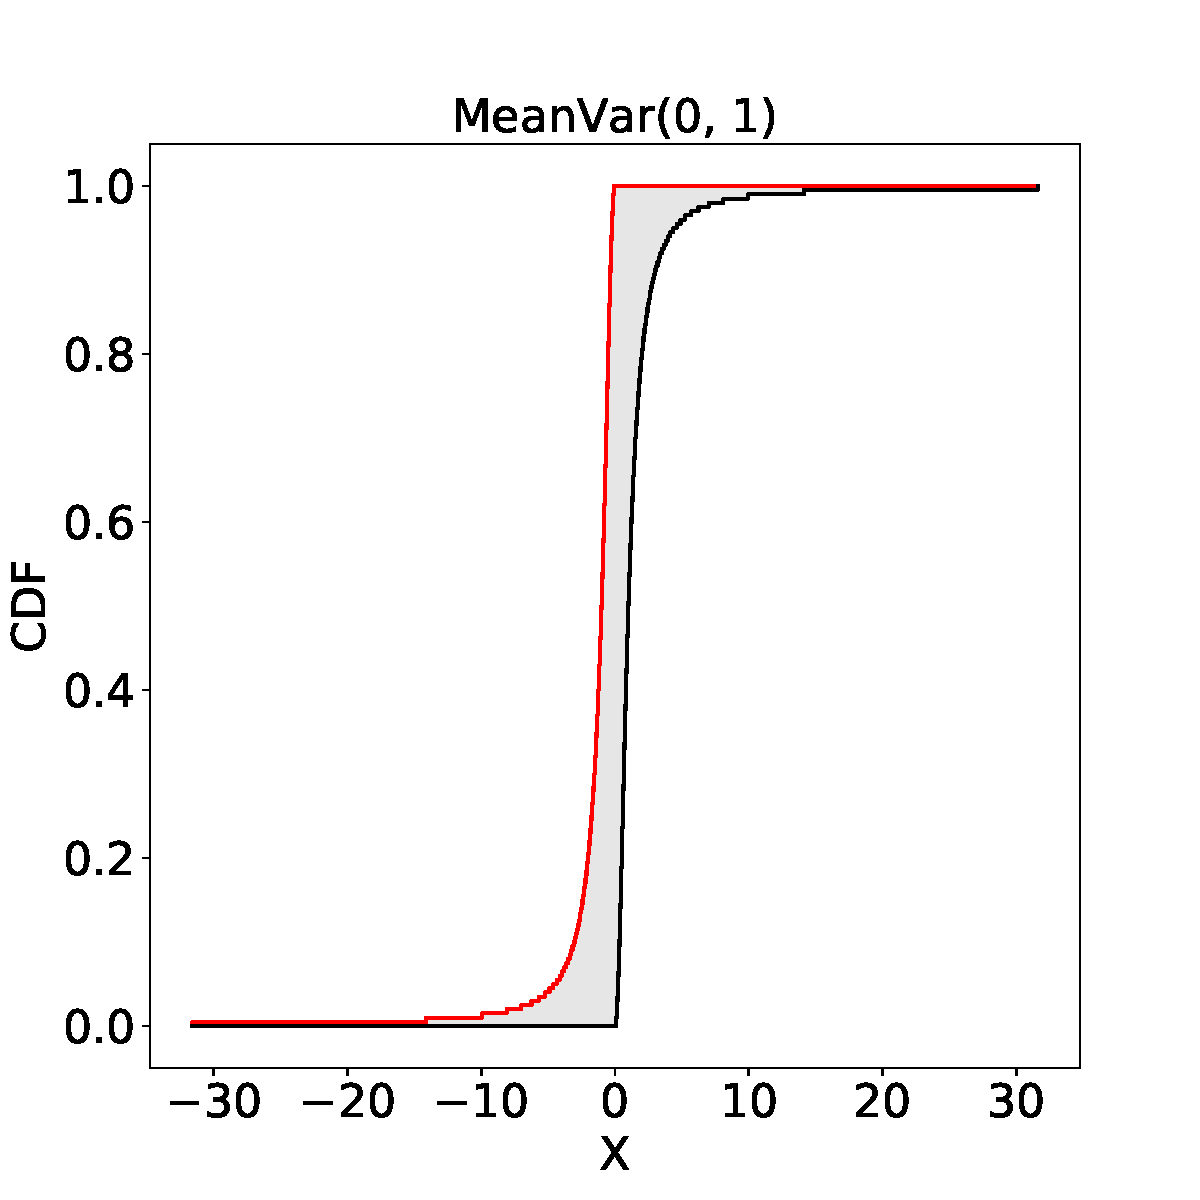
\includegraphics[width=.25\textwidth]{../examples/JuliaCon/fig6/fig6_pbox1.pdf}\hfill
  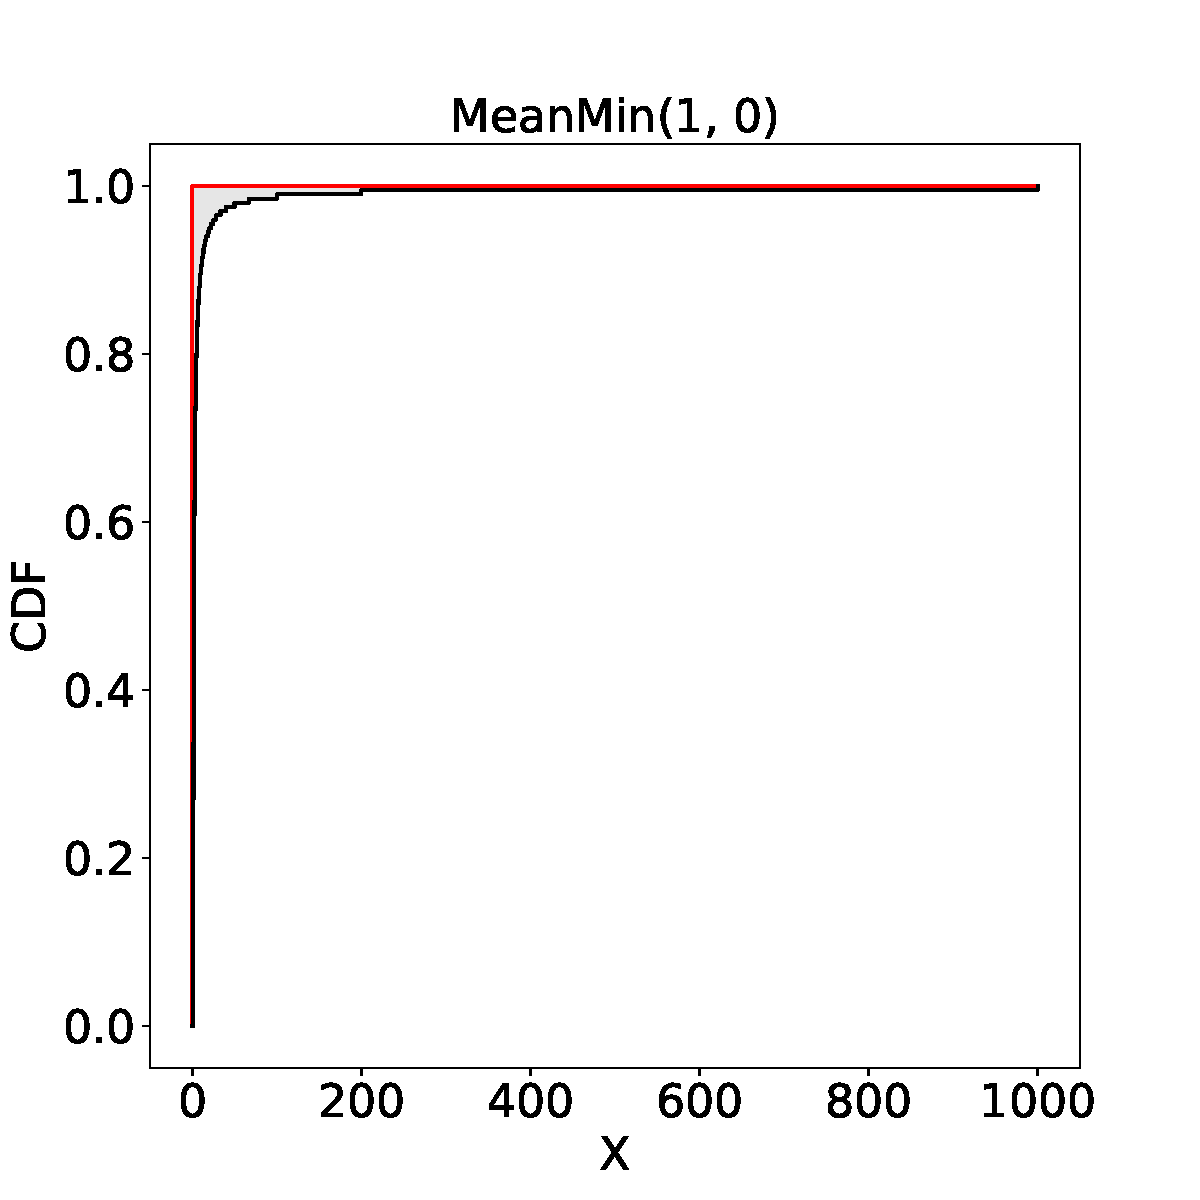
\includegraphics[width=.25\textwidth]{../examples/JuliaCon/fig6/fig6_pbox2.pdf}\hfill
  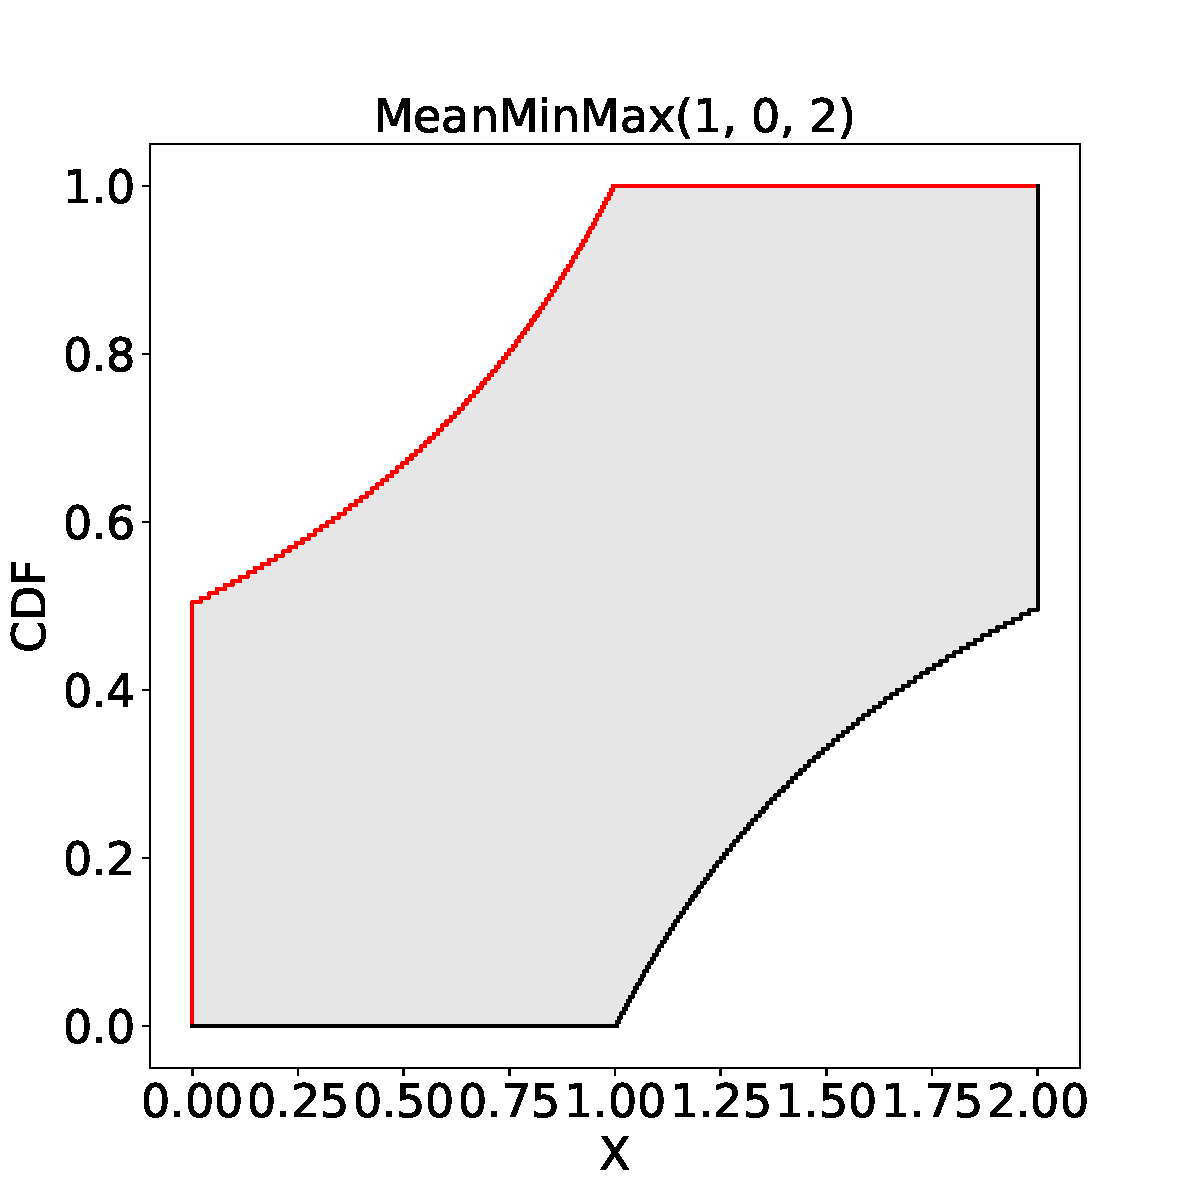
\includegraphics[width=.25\textwidth]{../examples/JuliaCon/fig6/fig6_pbox3.pdf}\hfill
  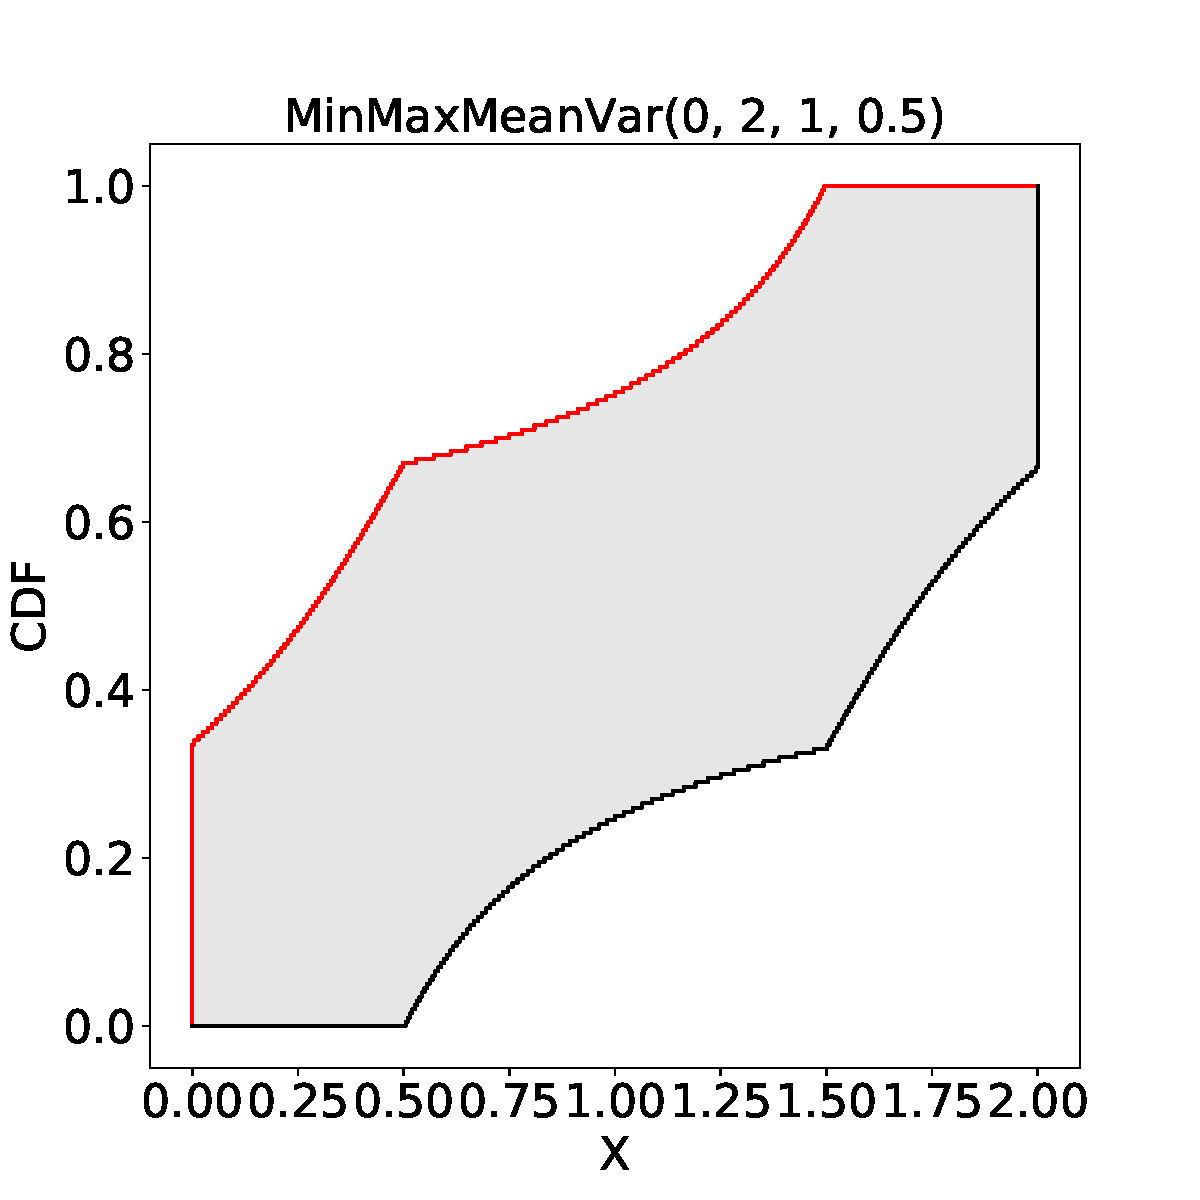
\includegraphics[width=.25\textwidth]{../examples/JuliaCon/fig6/fig6_pbox4.pdf}
  

  \caption{Examples of distribution-free p-boxes, constructed from various range and moment constrains.}
  \label{fig:figure6}
  
\end{figure*}


\begin{lstlisting}[language = Julia]
  function cdf(F :: pbox, x :: Real)
    
    u = F.u; d = F.d; n = length(u);
    
    cdf_u = 1 - sum(x .< u)/n;
    cdf_d = 1 - sum(x .<= d)/n;
    
    return interval(cdf_d, cdf_u)
  end

\end{lstlisting}

A horizontal cut (an evaluation of the inverse cdf) and a sample of a p-box can be found as follows: 

\begin{lstlisting}[language = Julia]
  import Base: rand

  function cut(F :: pbox, p :: Real)

    u = F.u; d = F.d; n = length(u);
    ps = range(0, 1, length = n+1);

    ind_u = findlast(ps[1:end-1] .<= p)
    ind_d = findfirst(ps[2:end] .>= p)
    
    return interval(u[ind_u], d[ind_d])
  end

  # a random sample is a random cut
  rand(F :: pbox, N :: Int) = cut.([F], rand(N))

\end{lstlisting}

And finally the probability measure, which we call the \textit{mass} for short:

\begin{lstlisting}[language = Julia]
  function mass(F :: pbox, x :: Interval)

    cdfHi = cdf(F, x.hi)  
    cdfLo = cdf(F, x.lo)  # returns intervals

    ub = cdfHi.hi - cdfLo.lo
    lb = max(0, cdfHi.lo - cdfLo.hi)

    return interval(lb, ub)
  end

\end{lstlisting}

Other available functions on p-boxes which we do not describe here are:

\begin{itemize}
  \item \textbf{env} or $\cup$: takes the envelope or hull of two p-boxes. A convex set-union of the probability sets
  \item \textbf{imp} or $\cap$: imposition or intersection of two p-boxes. Set-intersection of probability sets
  \item \textbf{subseteq} or $\subseteq$: checks if a p-box is a subset or equal to another
  \item \textbf{in} or $\in$: checks if a distribution is a member of a p-box
  \item \textbf{mixture}: a stochastic mixture of p-boxes.
\end{itemize}

\subsection{Where do p-boxes come from?}

In this section we discuss some situations where p-boxes arise naturally.


\subsubsection{Partial distributional information} \hfill \break

In situations where the parametric family of the uncertainty is known, for example it is known that $X$ is normally distributed $X \sim N(\mu_{X}, \sigma_{X}^{2})$ or that $Y$ is a uniform $Y \sim U(a_{Y},b_{Y})$, but the precise parameters to these functions are unknown, then p-boxes are a natural representation. In the case that bounds are known on parameters, then bounds on the cdf can be found using the interval parameters and the inverse cdf of the parametric family. Figure \ref{fig:figure3} shows a variety of p-boxes constructed this way.


\subsubsection{Missing family but partial moment information} \hfill \break
\label{section:Moments}

It is well known that generally a random variables distribution function cannot be uniquely determined solely from its moment information, even with an infinite number of moments, unless some assumptions are made about the family (i.e. it's normal). In probability theory this is known as the \textit{moment problem}. However, in these situations it is possible to define a p-box which bounds all random variables with the known properties, without loss of generality or making unwarranted assumptions.

These p-boxes are constructed using the Chebyshev (mean and variance) \cite{chebyshev1874valeurs}, Markov (mean and one bound) \cite{markoff1900question} and Cantelli (mean and range) inequalities from probability theory. These inequalities allow for the cdf to be bounded from various range and moment information. For example, the Chebyshev inequality can be used to find p-box bounds from the random variables mean and variance:

\begin{equation*}
  \underline{F}_{X}(x) = \begin{cases} 1 / (1 + (x - \mu_{X})^2 / \sigma^{2}_{X}),& \text{if } \mu_{X}<x \\
    1,& \text{if } x\leq \mu_{X} \end{cases}
\end{equation*}

\begin{equation*}
  \overline{F}_{X}(x)  = \begin{cases} 1 / (1 + \sigma^{2}_{X}/(x - \mu_{X})^2),& \text{if } x<\mu_{X} \\
  1,& \text{if } \mu_{X}\leq x \end{cases}
\end{equation*}

A list of available distribution-free constructors are:

\begin{itemize}
  \item \textbf{MeanVar (or MeanStd)}: using Chebyshev
  \item \textbf{MeanMin}: using Markov
  \item \textbf{MeanMax}: using Markov
  \item \textbf{MeanMinMax}: using Cantelli
  \item \textbf{MinMaxMeanVar (or MinMaxMeanStd)}: using a mix of inequalities
\end{itemize}

All distribution-free constructors may also take interval moments parameters.

\subsubsection{Operations involving intervals and distributions} \hfill \break

An arithmetic operation involving an interval and a precise distribution will produce set of distributions, i.e. a unique distribution for every real number in the interval, whose p-box bounds can be found. The following function performs a binary operation between a p-box and an interval:

\begin{lstlisting}[language = Julia]
  using MomentArithmetic

  function binary(F :: pbox, X :: Interval, op)

    u_z = op.(Interval.(F.u), X)
    d_z = op.(Interval.(F.d), X)

    u_z_ = getfield.(u_z, :lo)  # get right edges
    d_z_ = getfield.(d_z, :hi)  # get left edges

    # for moments
    F_range = interval(F.u[1], F.d[end])
    F_moms = Moments(F.m, F.v, F_range);
    Z_moms = op(F_moms, X);

    return pbox(u_z_, d_z_, Z_moms.mean, 
    Z_moms.var, F.shape)
  end
\end{lstlisting}

How the moment transformations are performed are not described here, however they are available in \texttt{MomentArithmetic.jl}\footnote{https://github.com/AnderGray/MomentArithmetic.jl} \cite{ferson2021distribution}. Figure \ref{fig:figure4} shows an example of an operation between a precise distribution and an interval.


\begin{figure}[htp]

  \centering
  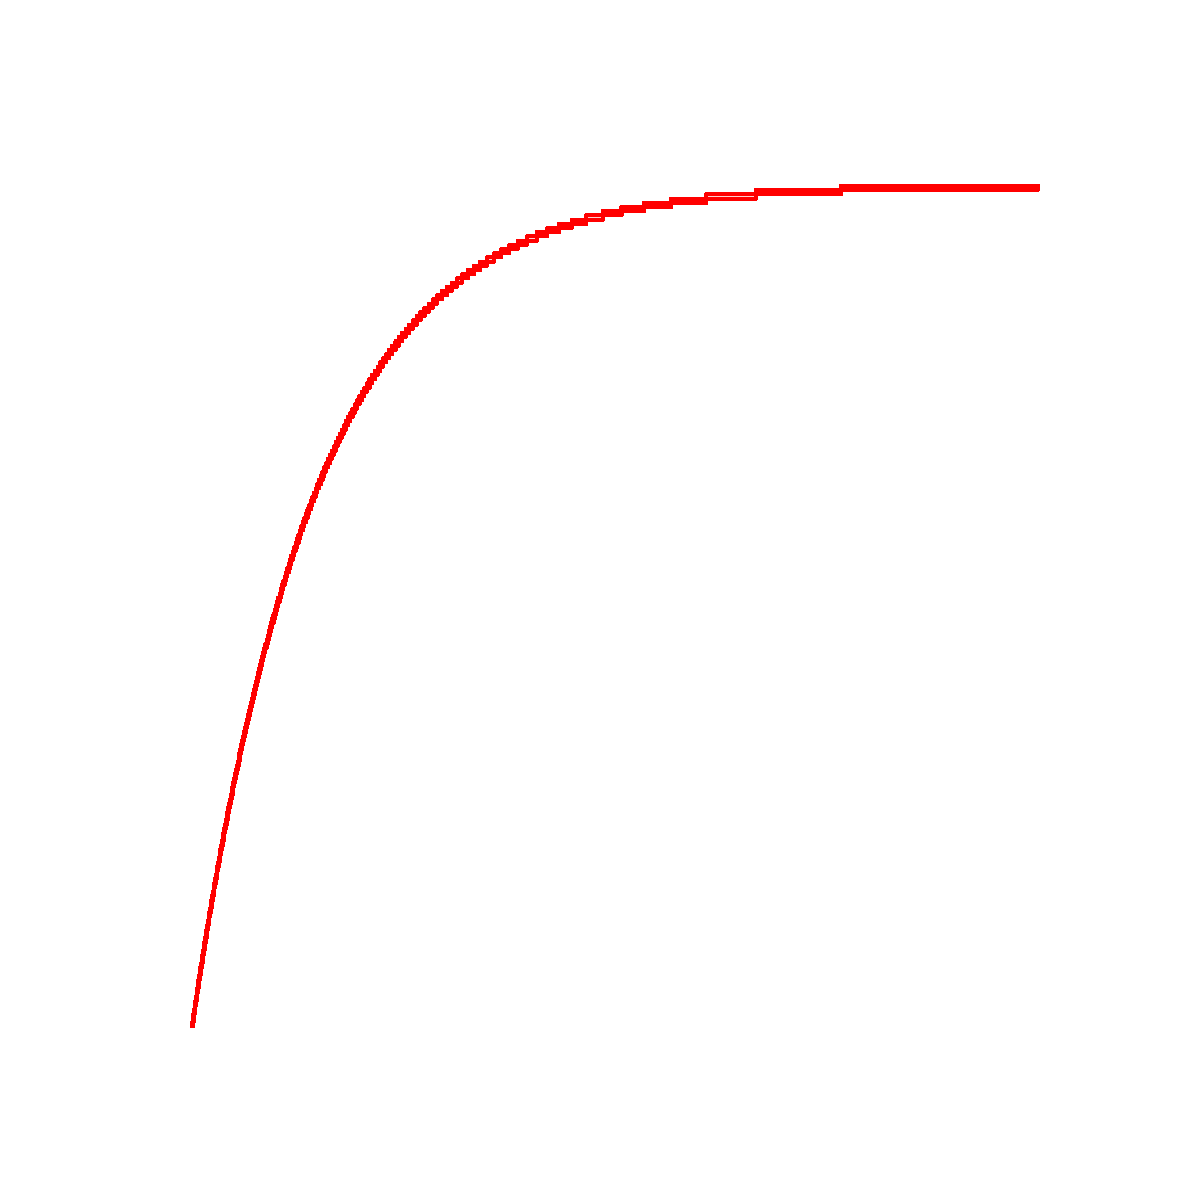
\includegraphics[width=0.12\textwidth]{../examples/JuliaCon/fig4/fig4_dist.pdf}
  \raisebox{8.0mm}{\noindent\Large*}
  
\includegraphics[width=0.12\textwidth]{../examples/JuliaCon/fig4/fig4_in.pdf}
  \raisebox{9.0mm}{{\Large$\rightarrow$}}
  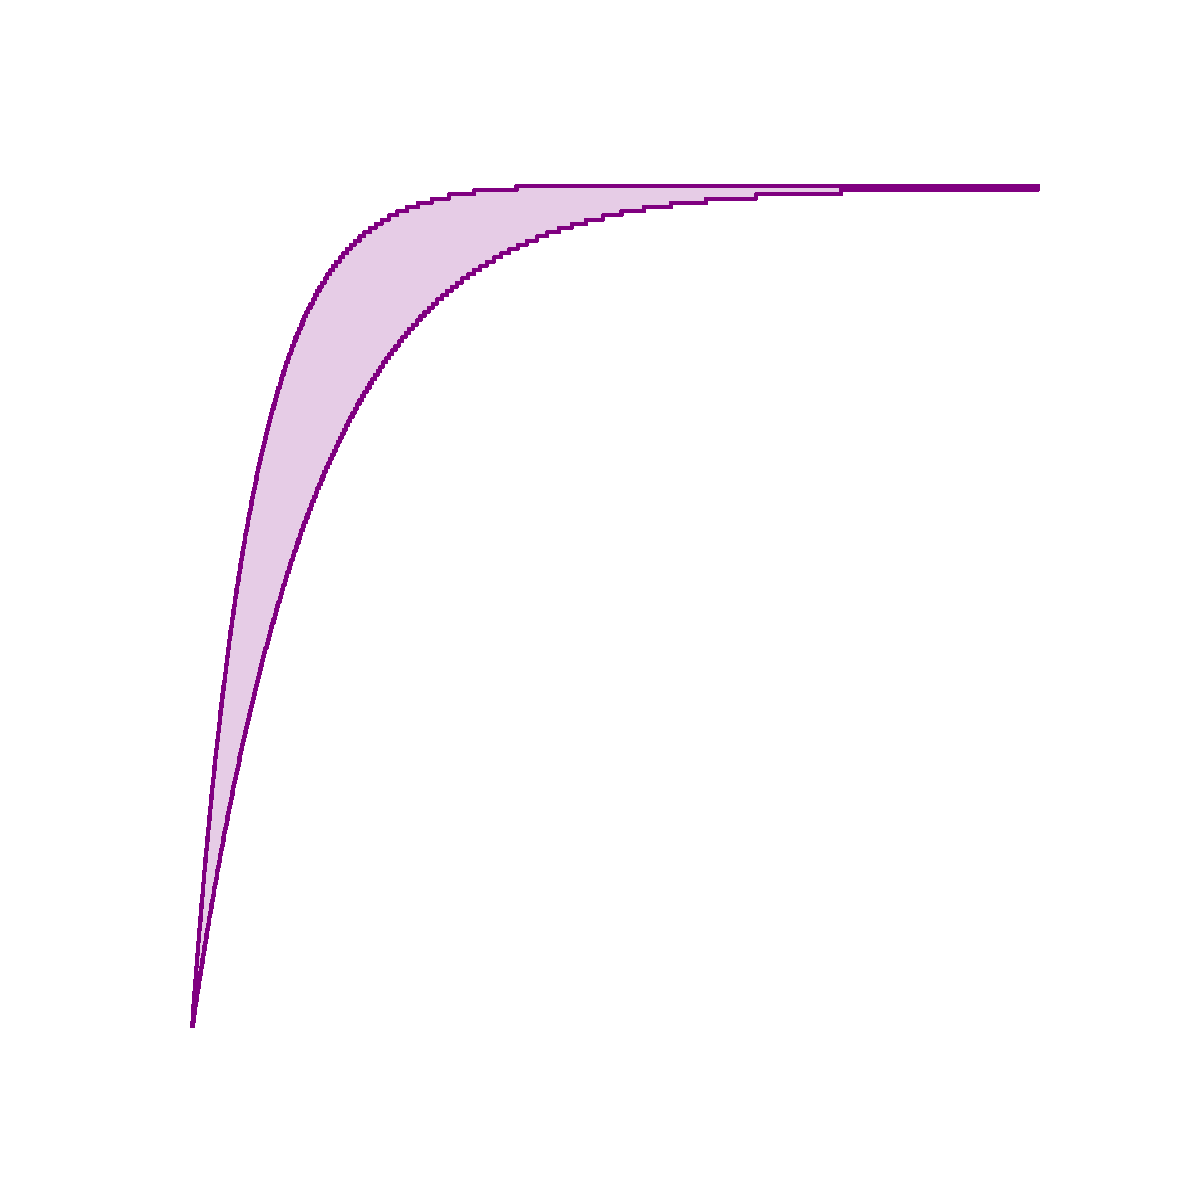
\includegraphics[width=0.12\textwidth]{../examples/JuliaCon/fig4/fig4_pbox.pdf}
  

  \caption{Illustration of a p-box resulting from a binary operation between a distribution and an interval.}
  \label{fig:figure4}
  
\end{figure}


\subsubsection{When dependencies between distributions are unknown} \hfill \break

In the case where a binary operation is performed between two distributions but whose dependence or correlation is unknown, a single output distribution cannot be defined. However a bounding p-box can be computed. This is the original question of Kolmogorov as described in the introduction. We call such operations between p-boxes where the marginals are fixed but no joint information is known \textit{Fréchet} operations, after the mathematician Maurice R. Fréchet, who first discovered how to bound joint distributions with fixed marginals \cite{frechet1935generalisation}. How operations between p-boxes with partial or no dependence information is known is described in section \ref{sec:pboxBinary}. Figure \ref{fig:figure5} illustrates a Fréchet operation between a uniform and a normal distribution.

\begin{figure}[htp]

  \centering
  
\includegraphics[width=0.12\textwidth]{../examples/JuliaCon/fig5/fig5_dist1.pdf}
  \raisebox{8.0mm}{\noindent\Large+\small$_{\text{Fr{\'e}chet}}$}
  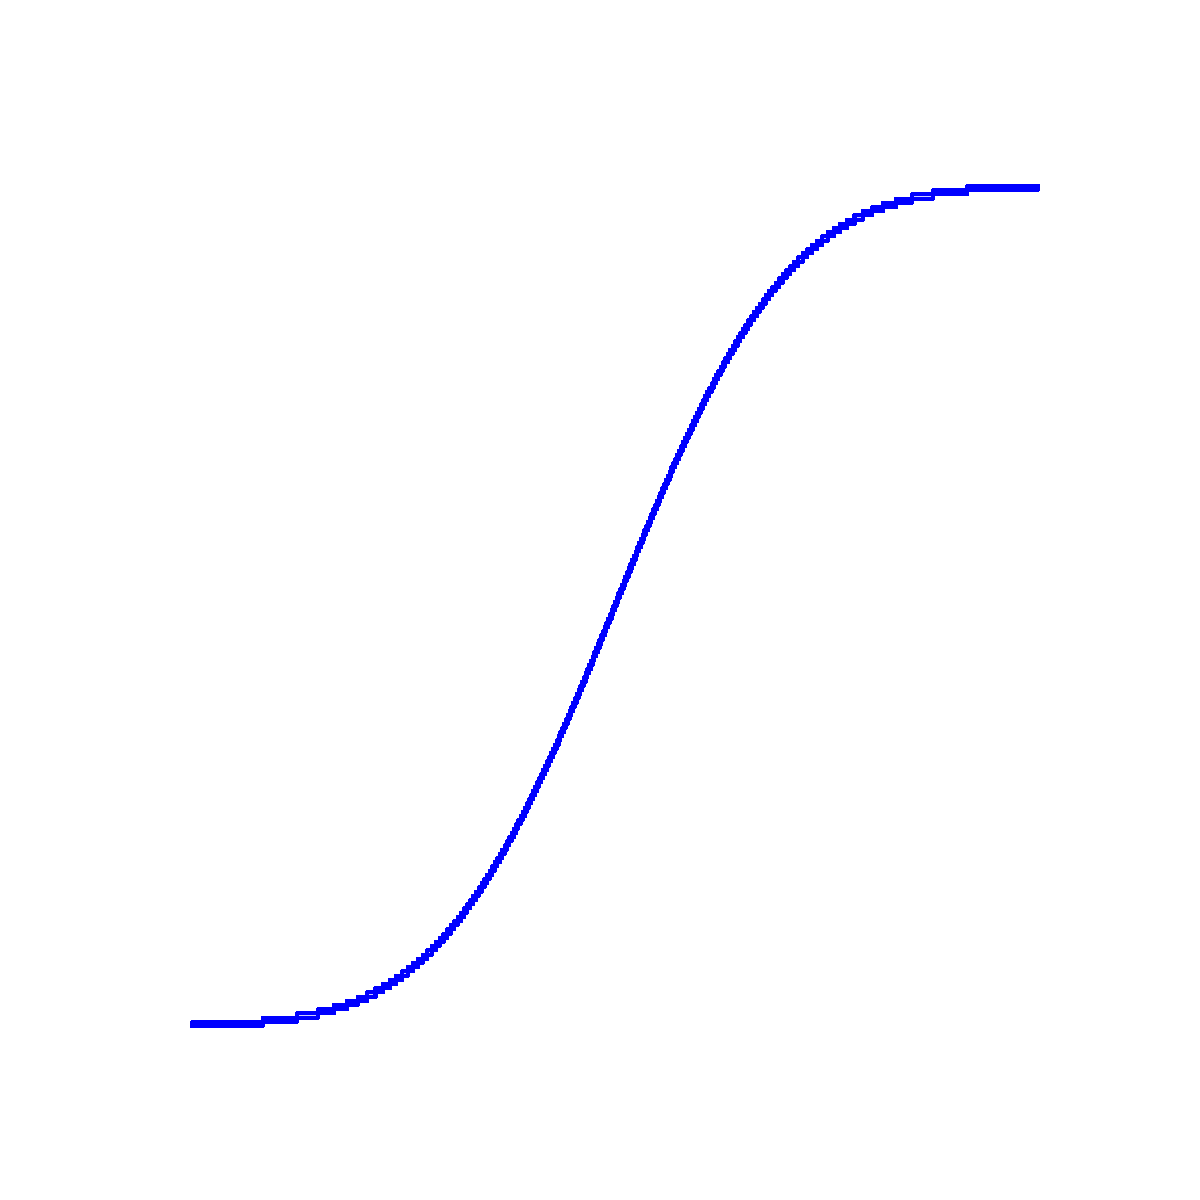
\includegraphics[width=0.12\textwidth]{../examples/JuliaCon/fig5/fig5_dist2.pdf}
  \raisebox{9.0mm}{{\Large$\rightarrow$}}
  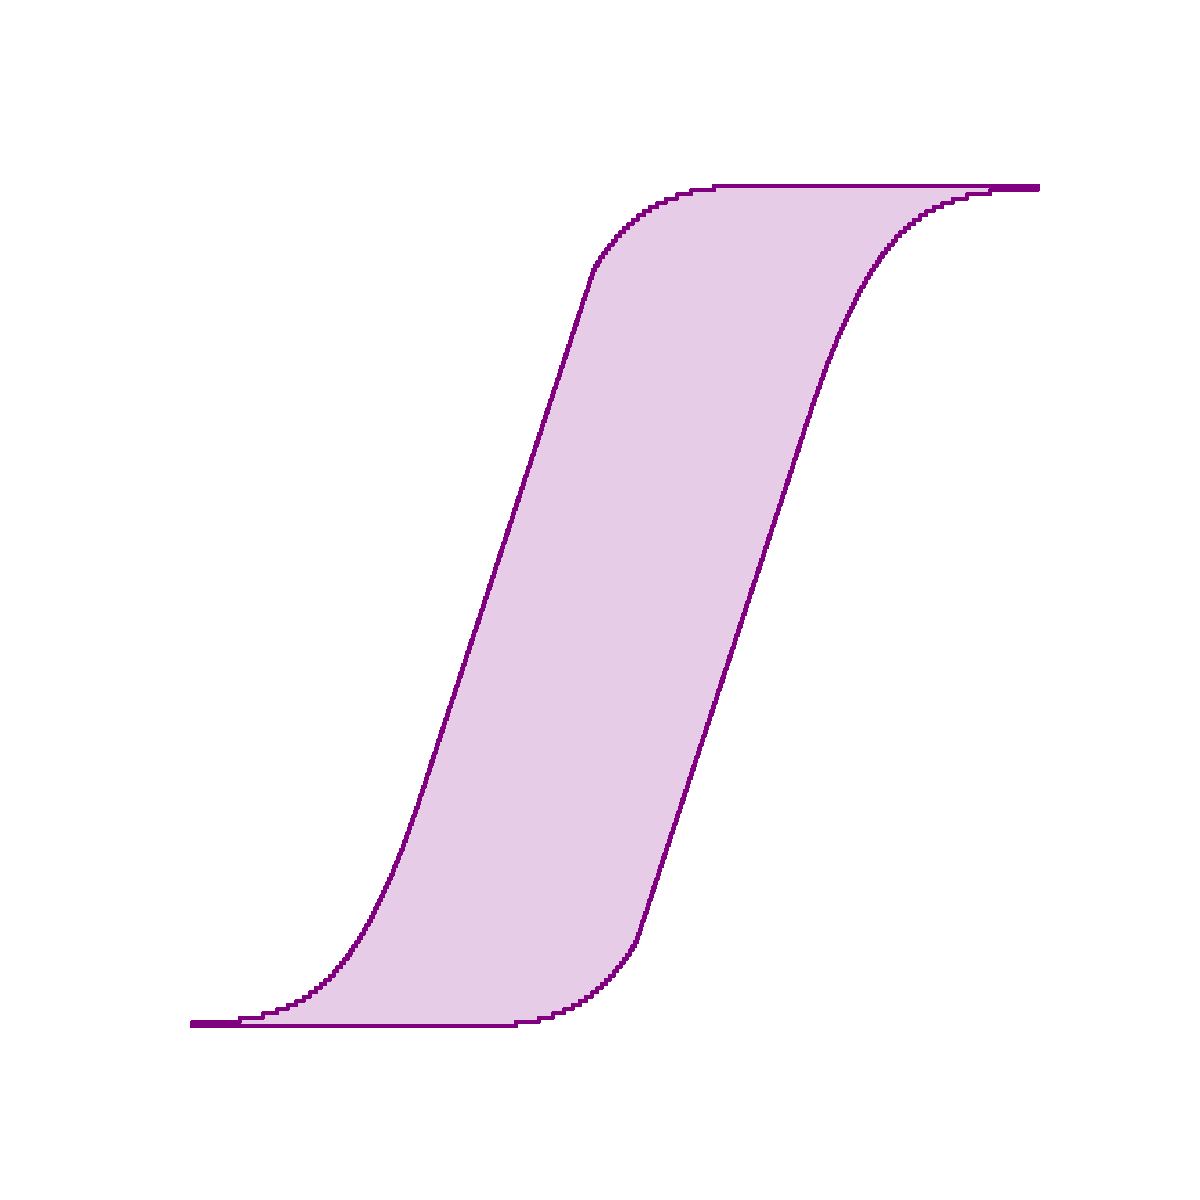
\includegraphics[width=0.12\textwidth]{../examples/JuliaCon/fig5/fig5_pbox.pdf}
  

  \caption{Illustration of a p-box resulting from a Fréchet operation}
  \label{fig:figure5}
  
\end{figure}


\subsubsection{Outer approximations of precise distributions} \hfill \break

Outer approximations of precise distributions described in section \ref{sec:outer_approx} also lead naturally to a p-box. All probabilistic quantities of discretised distribution functions will be intervals, which shrink to precise quantities as the discretisation increases. In that sense, both distributions functions and p-boxes are p-boxes in \texttt{ProbabilityBoundsAnalysis.jl}.

\subsubsection{Inferential methods when data is limited or bad} \hfill \break

Probability distributions are almost always constructed from data or measurements, or otherwise are assumed as a model or derived from expert opinion. Usually to construct a probability distribution accurately, a large amount of high quality data is required. P-boxes arise naturally when this is not the case, for example if the data are intervals instead of points, or when data is sparse or not reliable, and an exact distribution function is difficult to prescribe.

An example is robust Bayesian analysis, where the analyst does not have enough information to reliably establish a single prior and likelihood function, but instead has a collection of priors and likelihoods, leading to a set of posteriors distributions, to which a p-box can be identified.

A method which is growing in popularity are inferential models \cite{martin2015inferential}. These generalise classical inference methods to account for limited statistical knowledge, and give a statistical inference theory which is non-additive (as opposed to classical probability which is additive). These inference procedures, often based on random sets, give certain validity and performance guarantees. Inferential models can viewed from the perspective of bounding sets of distributions, and is closely linked to possibility theory \cite{liu2020inferential}. A p-box can be prescribed to such structures, leading to structures like confidence boxes or c-boxes \cite{fersoncomputing}, which follow the same arithmetic rules as p-boxes. 

\iffalse
\subsection{Relationship to other ideas}

\subsubsection{Random set theory}

\subsubsection{Possibility theory}
\fi

%\section{Operations on p-boxes}

%\section{P boxes}

\subsection{Bivariate p-boxes}

P-boxes have been extended to higher dimensions \cite{montes2015sklar}, however like with precise probabilities, when considering multivariate p-boxes the dependence information (like correlation) must be accounted for. Considering complex dependencies amongst p-boxes is important, as they play a key role in binary operations. That is, the result of an operation between two p-boxes not only depends on the input p-boxes, but also how the inputs are correlated.

Covariance, and subsequently the pearson correlation coefficient, is insufficient to fully determine the dependence between two random variables. Like for the univariate moments, a single multivariate distribution cannot be prescribed for a given value of the covariance without making distributional assumptions (like normality). A more descriptive (and general) model for dependence is required to exactly specify a multivariate distribution.

Copulas \cite{nelsen2007introduction} provide a solution to this problem. A copula is a multivariate cdf with uniform marginals on the interval $[0, 1]$. A copula is a multivariate distribution which has all marginal (univariate) information stripped away, leaving only the dependency. All dependence information can therefore be encoded in a copula exactly and completely separately from its marginals. Often multivariate problems in probability can be reduced to an analysis of copulas.

A bivariate copula (2-copula) $C$ is any function $C:[0,1]^2 \rightarrow [0,  1]$ with the following properties:

\begin{enumerate}
  \item Grounded: $C(0,v) = C(u,0) = 0$,
  \item Uniform margins: $C(u,1) = u; \;C(1,v) = v$,
  \item 2-increasing: \\ $C(u_{2},v_{2}) - C_{}(u_{2}, v_{1}) - C(u_{1}, v_{2}) + C(u_{1}, v_{1}) \ge 0$\\ for all $0 \le u_{1} \le u_{2} \le 1$ and $0 \le v_{1} \le v_{2} \le 1$.
\end{enumerate}

Three important 2-copulas are:

\begin{align*}
  W(u,v) &= \mathrm{max}( u + v-1,0),  \\
  \Pi(u,v) &= uv, \\
  %\mathcal{P}(u,v) &= uv \\
  %\Pi(u,v) &= uv\\
  %\mu(u,v) &= uv \\
  %C_{\pi}(u,v) &=uv\\
  M(u,v) &= \mathrm{min}(u,v),
\end{align*}

where $W$ encodes maximally negative correlation, $\Pi$ encodes stochastic independence, and $M$ encodes maximally positive correlation. Moreover, $W$ and $M$ are bounds on all 2-copulas: $W(u,v) \leq C(u,v) \leq M(u,v)$. A bivariate cdf $F_{XY}$ can be constructed from two marginal cdfs $F_{X}$ and $F_{Y}$ and copula $C$ using Sklar's theorem:

\begin{equation*}
  F_{XY}(x,y) = C(F_{X}(x), F_{Y}(y)) ,
\end{equation*}

where the constructed bivariate distribution will follow the dependence encoded in the copula and have the prescribed marginals. Sklar's theorem also works in reverse, where the dependence can be extracted from a multivariate distribution: 

\begin{equation*}
  C(u,v) = F_{XY}(F^{-1}_{X}(u), F^{-1}_{Y}(v)) .
\end{equation*}

Copulas also give a very convenient way to sample from $F_{XY}$ in a generalisation of inverse transform sampling, where first the copula is sampled $(u,v) \sim C$, and then transformed through the inverses of the marginals $(F^{-1}_{X}(u), F^{-1}_{Y}(v))$.

Sklar's theorem has a straightforward imprecise extension \cite{montes2015sklar}, where the two bivariate bounds of a p-box $[\underline{F}_{XY}(x,y), \overline{F}_{XY}(x,y)]$ can expanded in terms of two marginal p-boxes and bounds on a copula $[\underline{C}(u,v), \overline{C}(u,v)]$: 

\begin{align*}
  \underline{F}_{XY}(x,y) &= \underline{C}(\underline{F}_{X}(x), \underline{F}_{Y}(y)), \\ 
  \overline{F}_{XY}(x,y) &= \overline{C}(\overline{F}_{X}(x), \overline{F}_{Y}(y)).
\end{align*}

Samples and the probability measure can also be found from a bivariate p-box. Like how a sample of a univariate p-box is an interval, a sample of a bivariate p-box will be an interval box, i.e. a two dimensional rectangular set. Multiple samples will therefore be a population of interval boxes, which together follow the dependency encoded in $C$. The bottom of Figure \ref{fig:figure7} shows 100 samples of a bivariate p-box, whose marginals are $X \sim \text{Beta}([4,8], 3)$ and $Y \sim \text{N}([0,2], 2)$, and with the Gaussian copula (multivariate normal's copula) with correlation coefficient $\rho_{XY} = -0.8$: $C = \Phi_{-0.8}$. The top of Figure \ref{fig:figure7} shows the cdf bounds. The probability measure from a bivariate p-box in the rectangular set $ U = [x_{1}, x_{2}] \times [y_{1}, y_{2}]$ is\footnote{Which is nearly a straightforward application of interval arithmetic to the precise calculation $F(x_{2}, y_{2}) - F(x_{1}, y_{2}) - F(x_{2}, y_{1}) + F(x_{1}, y_{1})$}: 

\begin{align*}
  \underline{\mathbb{P}}(U) &= \text{max}(0, \underline{F}(x_{2}, y_{2}) - \overline{F}(x_{1}, y_{2}) - \overline{F}(x_{2}, y_{1}) + \underline{F}(x_{1}, y_{1})) ,\\ 
  \overline{\mathbb{P}}(U)  &= \text{min}(1, \overline{F}(x_{2}, y_{2}) - \underline{F}(x_{1}, y_{2}) - \underline{F}(x_{2}, y_{1}) + \overline{F}(x_{1}, y_{1}) ).
\end{align*}


A minimal structure, cdf, random sample and probability measure of a bivariate p-box is \footnote{https://github.com/AnderGray/BivariateCopulas.jl}:

\begin{lstlisting}[language = Julia]
  using BivariateCopulas
  using BivariateCopulas: sample

  struct BivPbox{T <: Real}

    X :: pbox{T}  # 1st marginal
    Y :: pbox{T}  # 2nd marginal
    C :: copula   # copula

  end

  function cdf(F :: BivPbox, x :: Real, y :: Real)

    cdf_X = cdf(F.X, x)   # returns interval
    cdf_Y = cdf(F.Y, y)

    F_cdf_lo = F.C(cdf_X.lo, cdf_Y.lo)
    F_cdf_hi = F.C(cdf_X.hi, cdf_Y.hi)

    return interval(F_cdf_lo, F_cdf_hi)
  end

  function rand(F :: BivPbox, N :: Int)

    C_samps = sample(F.C, N)

    X_samps = cut.([F.X], C_samps[:, 1])
    Y_samps = cut.([F.Y], C_samps[:, 2])

    return IntervalBox.(X_samps, Y_samps)
  end

  function mass(F :: BivPbox, box :: IntervalBox)

    x = box.v[1]; y = box.v[2];  # gets intervals

    F_1 = cdf(F, x.lo, y.lo)
    F_2 = cdf(F, x.hi, y.lo)
    F_3 = cdf(F, x.lo, y.hi)
    F_4 = cdf(F, x.hi, y.hi)

    # using intervals
    mass = F_4 - F_3 - F_2 + F_1;

    return max(0, min(1, mass))
  end
\end{lstlisting}

\begin{figure}[htp]

  
  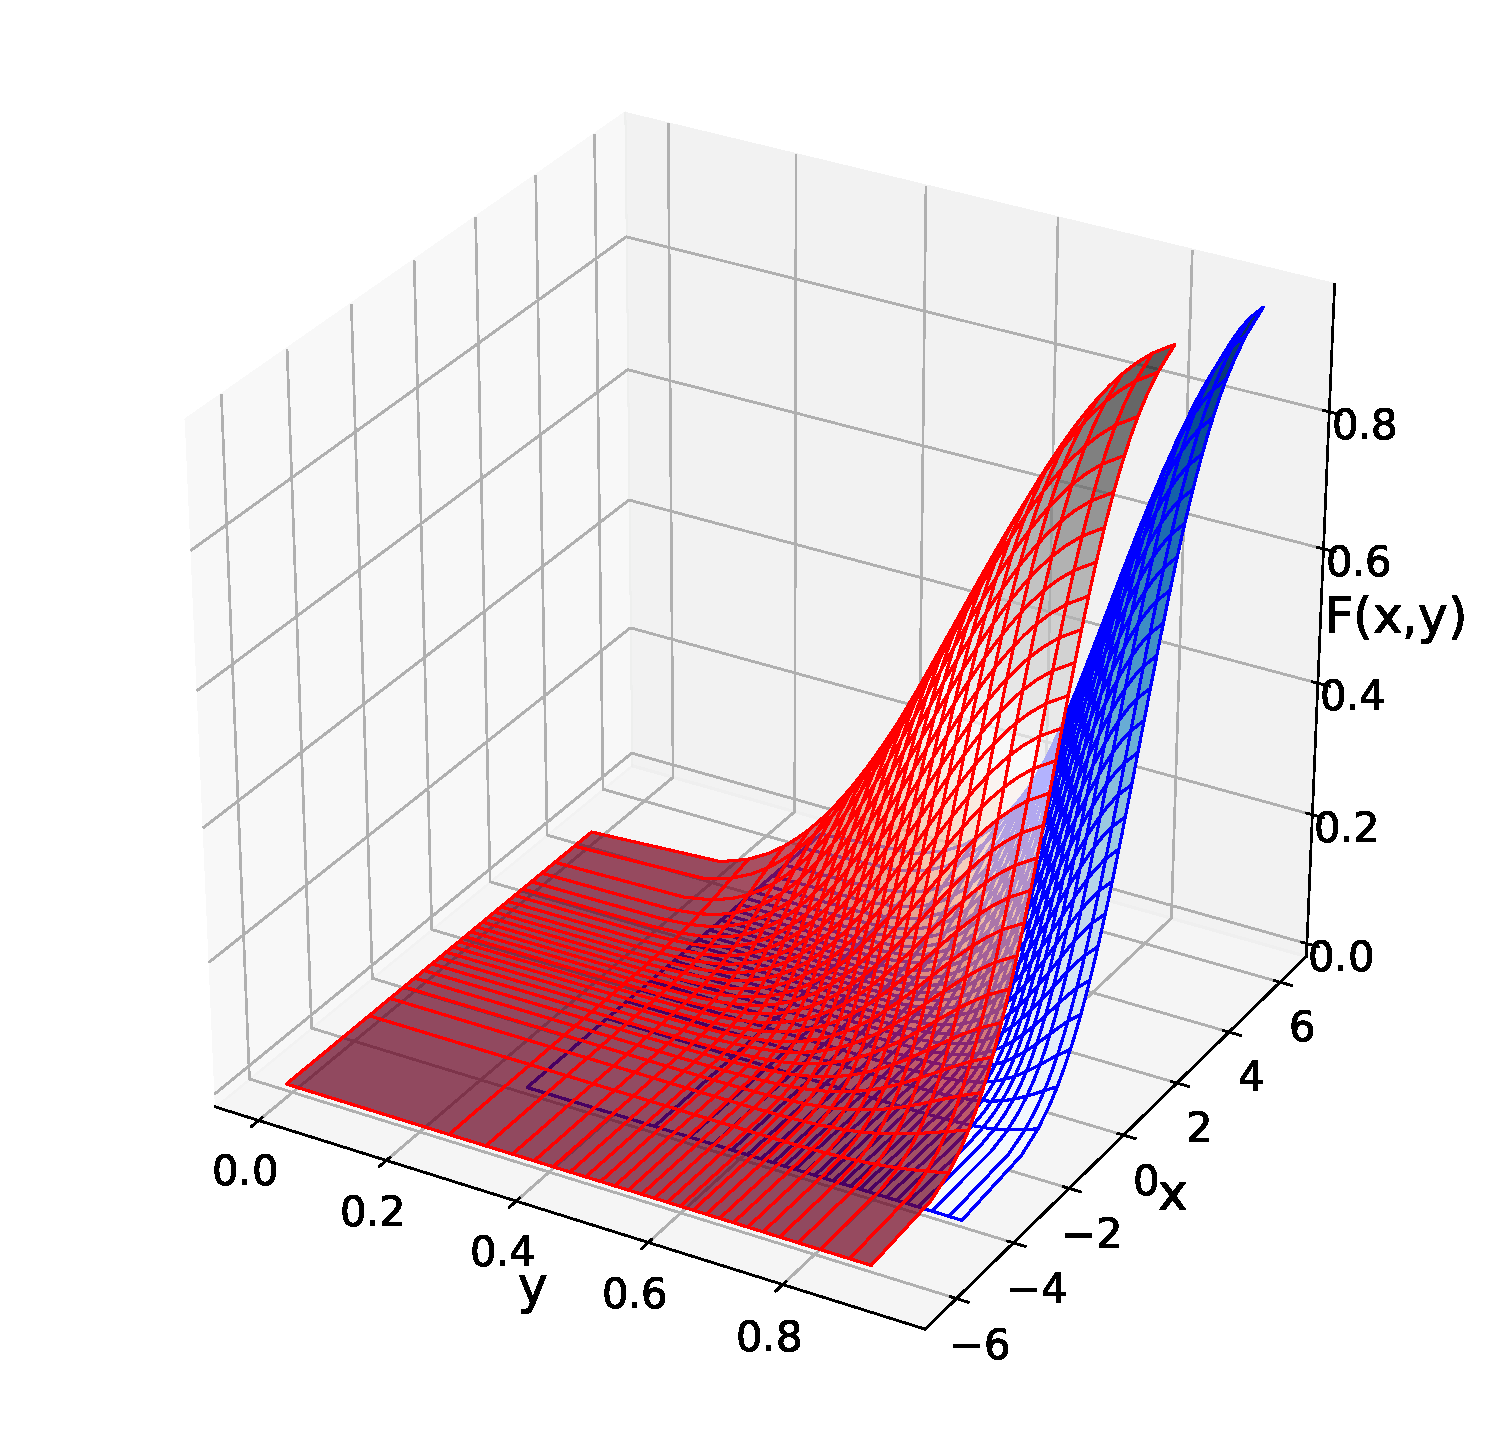
\includegraphics[width=0.5\textwidth]{../examples/JuliaCon/fig7/biv_cdf.pdf} 
  
  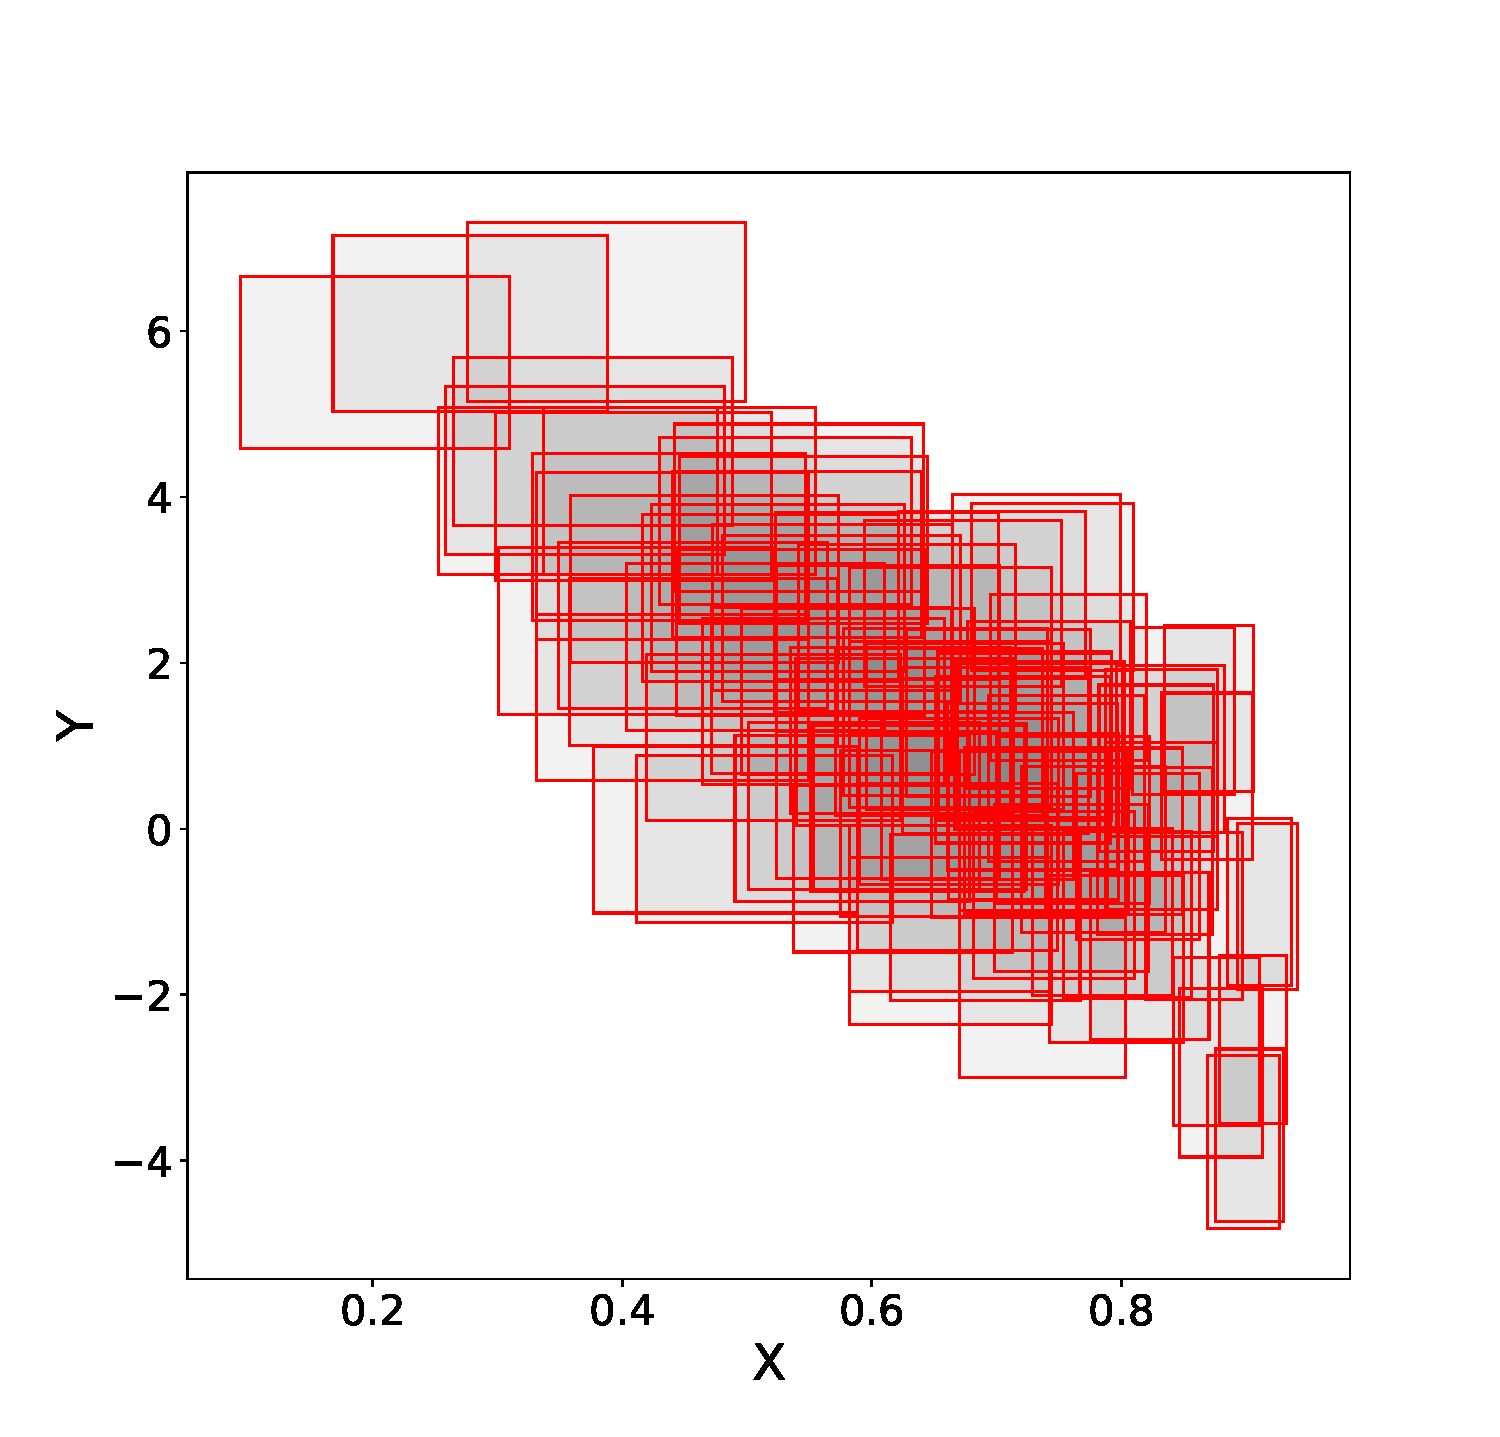
\includegraphics[width=0.5\textwidth]{../examples/JuliaCon/fig7/samples.pdf}
  

  \caption{Cdf bounds of a bivariate p-box (top) with $X \sim \text{Beta}([4,8], 3)$, $Y \sim \text{N}([0,2], 2)$, and $\rho_{XY} = -0.8$, and 100 samples (bottom)}
  \label{fig:figure7}
  
\end{figure}

\begin{figure*}[htp]

  \centering
  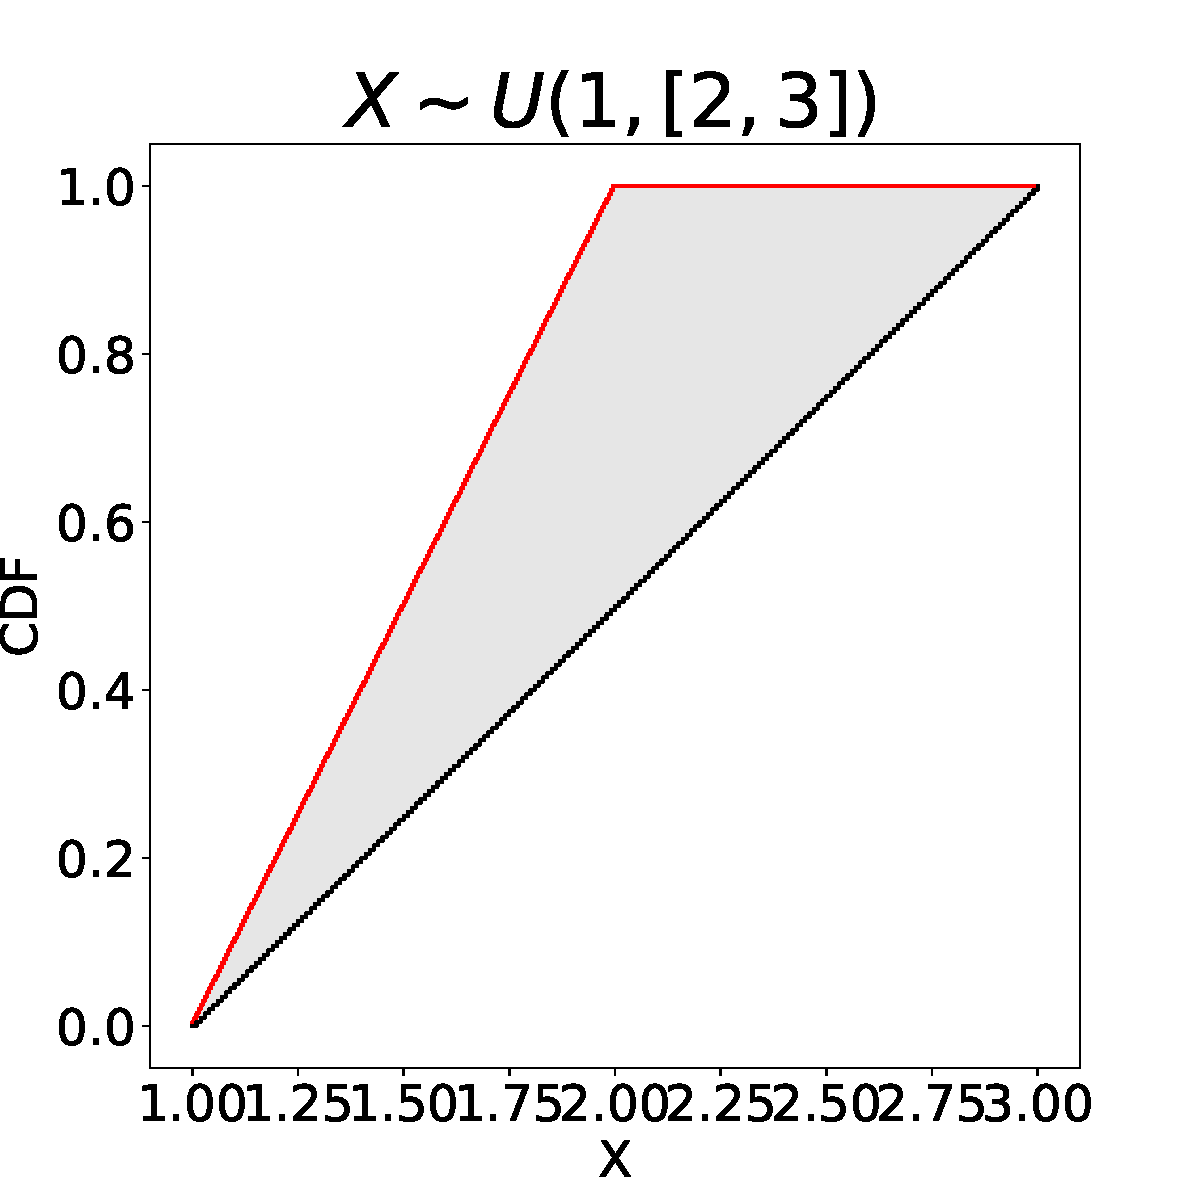
\includegraphics[width=.25\textwidth]{../examples/JuliaCon/fig8/fig8_pbox1.pdf}\hfill
  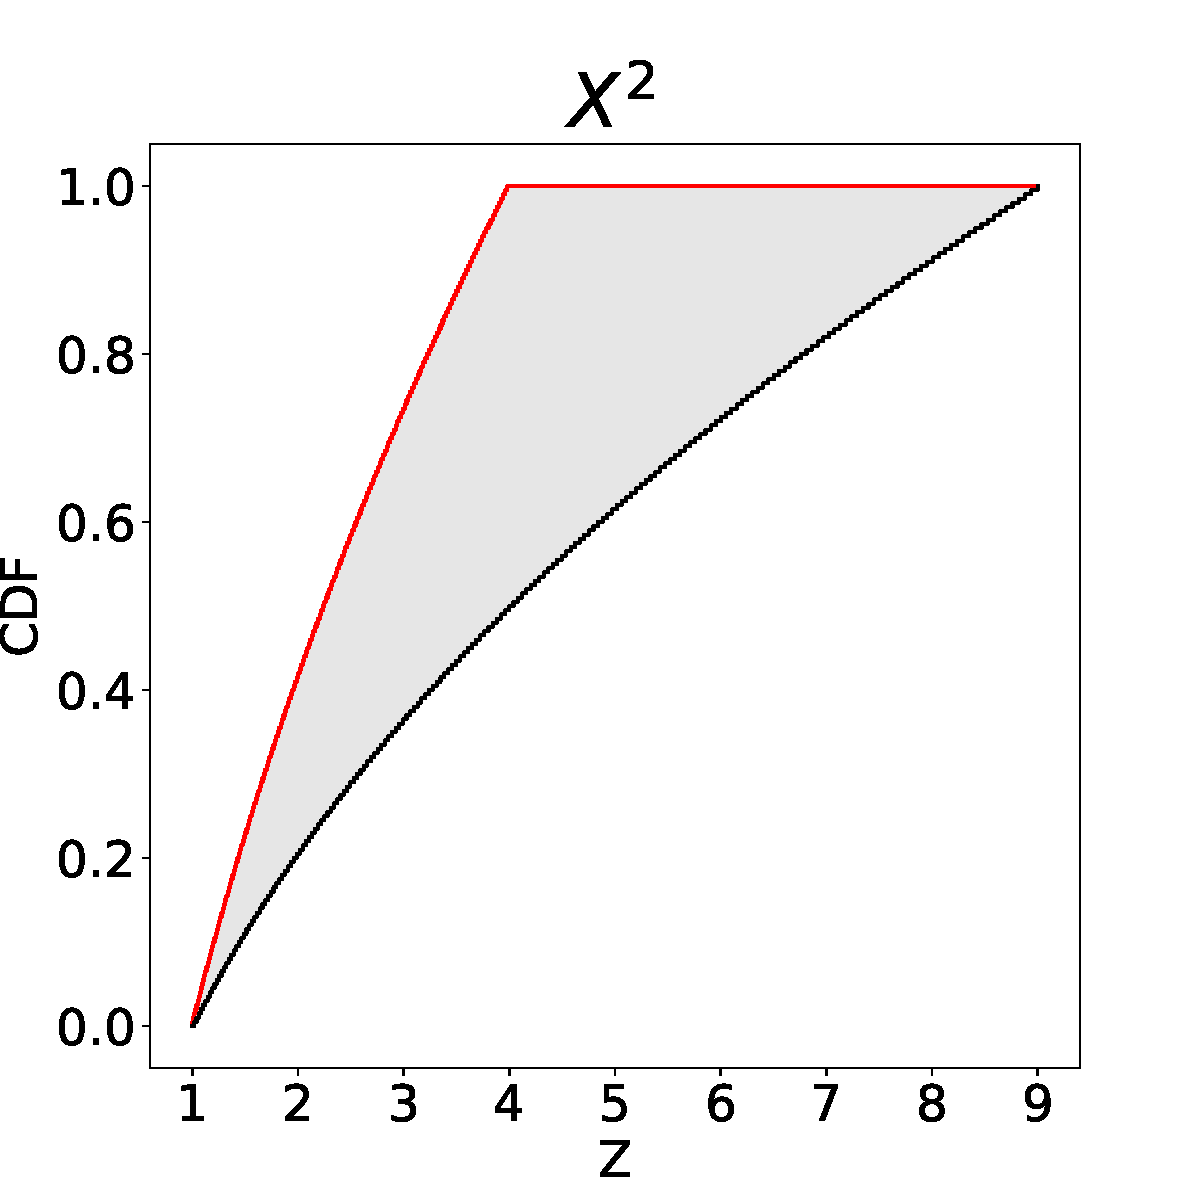
\includegraphics[width=.25\textwidth]{../examples/JuliaCon/fig8/fig8_pbox2.pdf}\hfill
  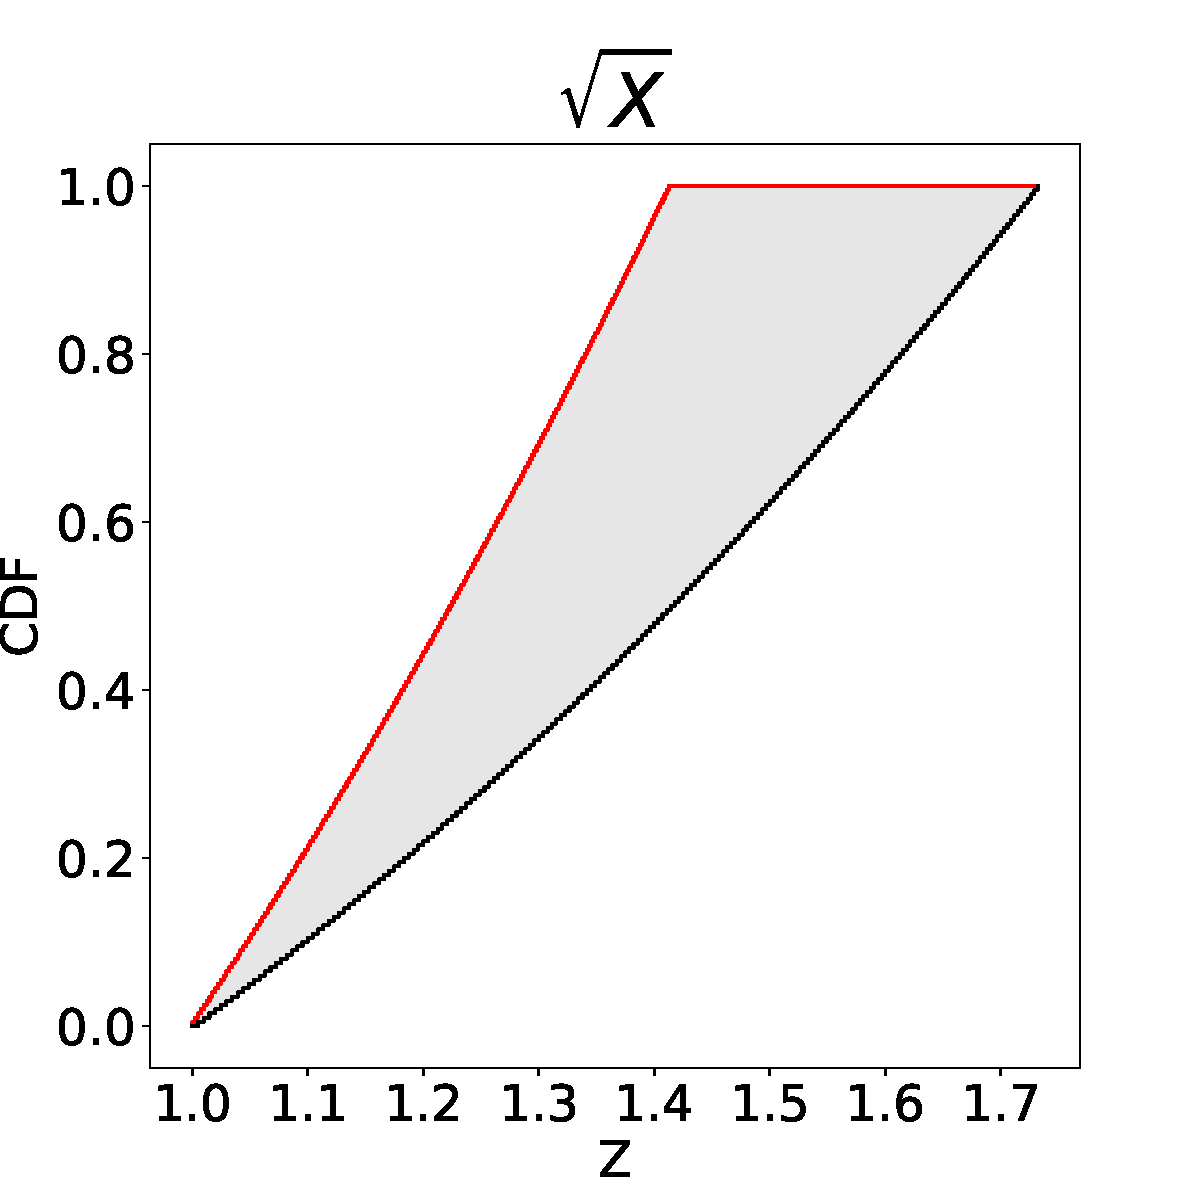
\includegraphics[width=.25\textwidth]{../examples/JuliaCon/fig8/fig8_pbox3.pdf}\hfill
  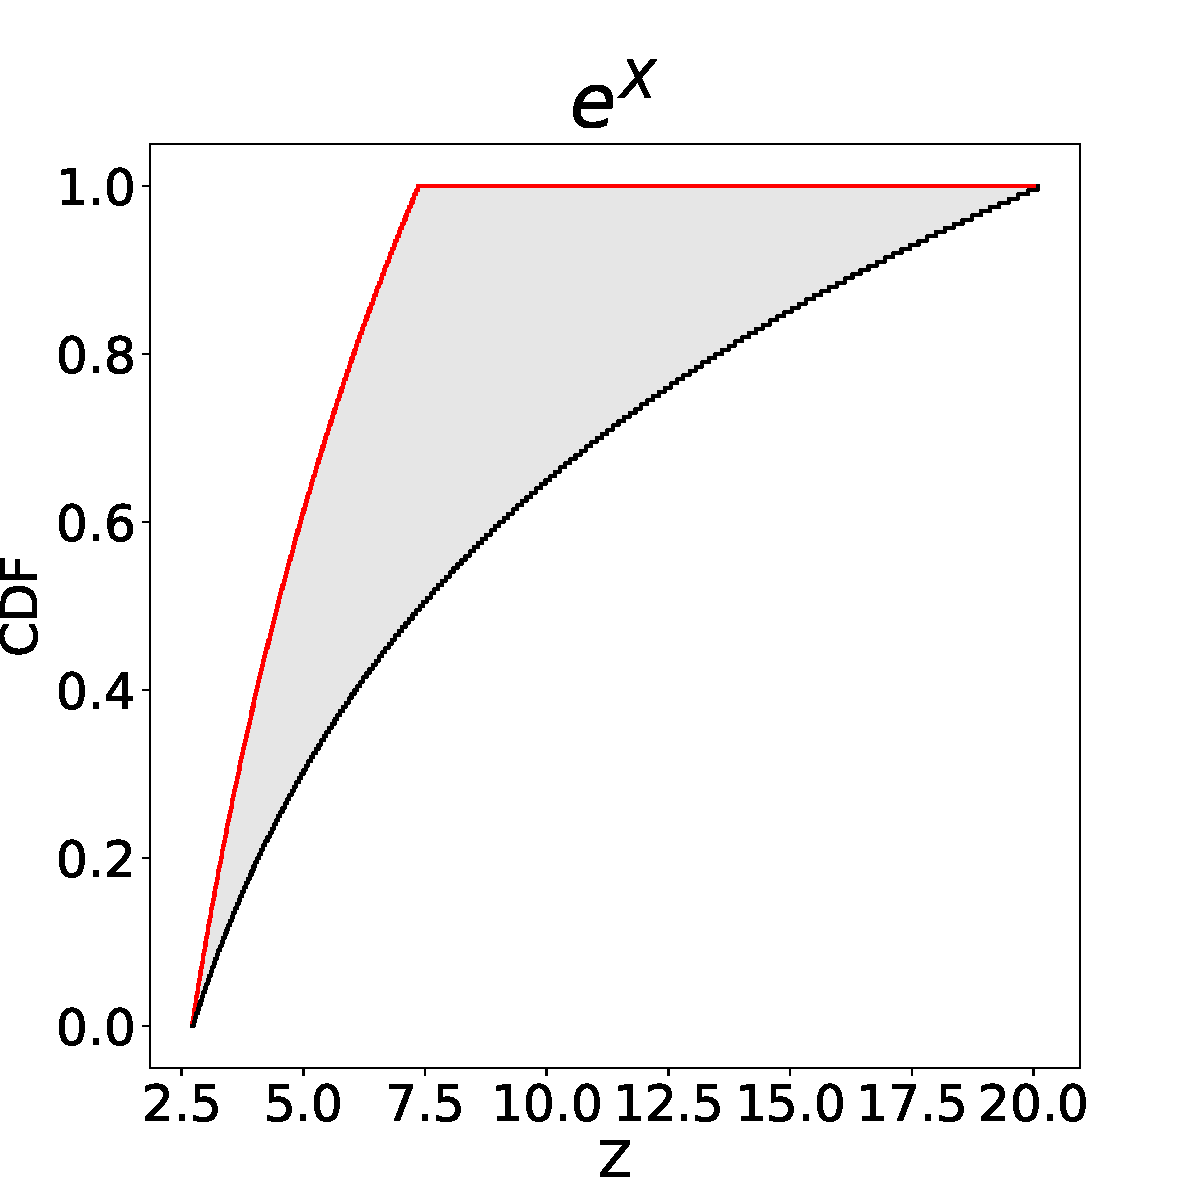
\includegraphics[width=.25\textwidth]{../examples/JuliaCon/fig8/fig8_pbox4.pdf}
  

  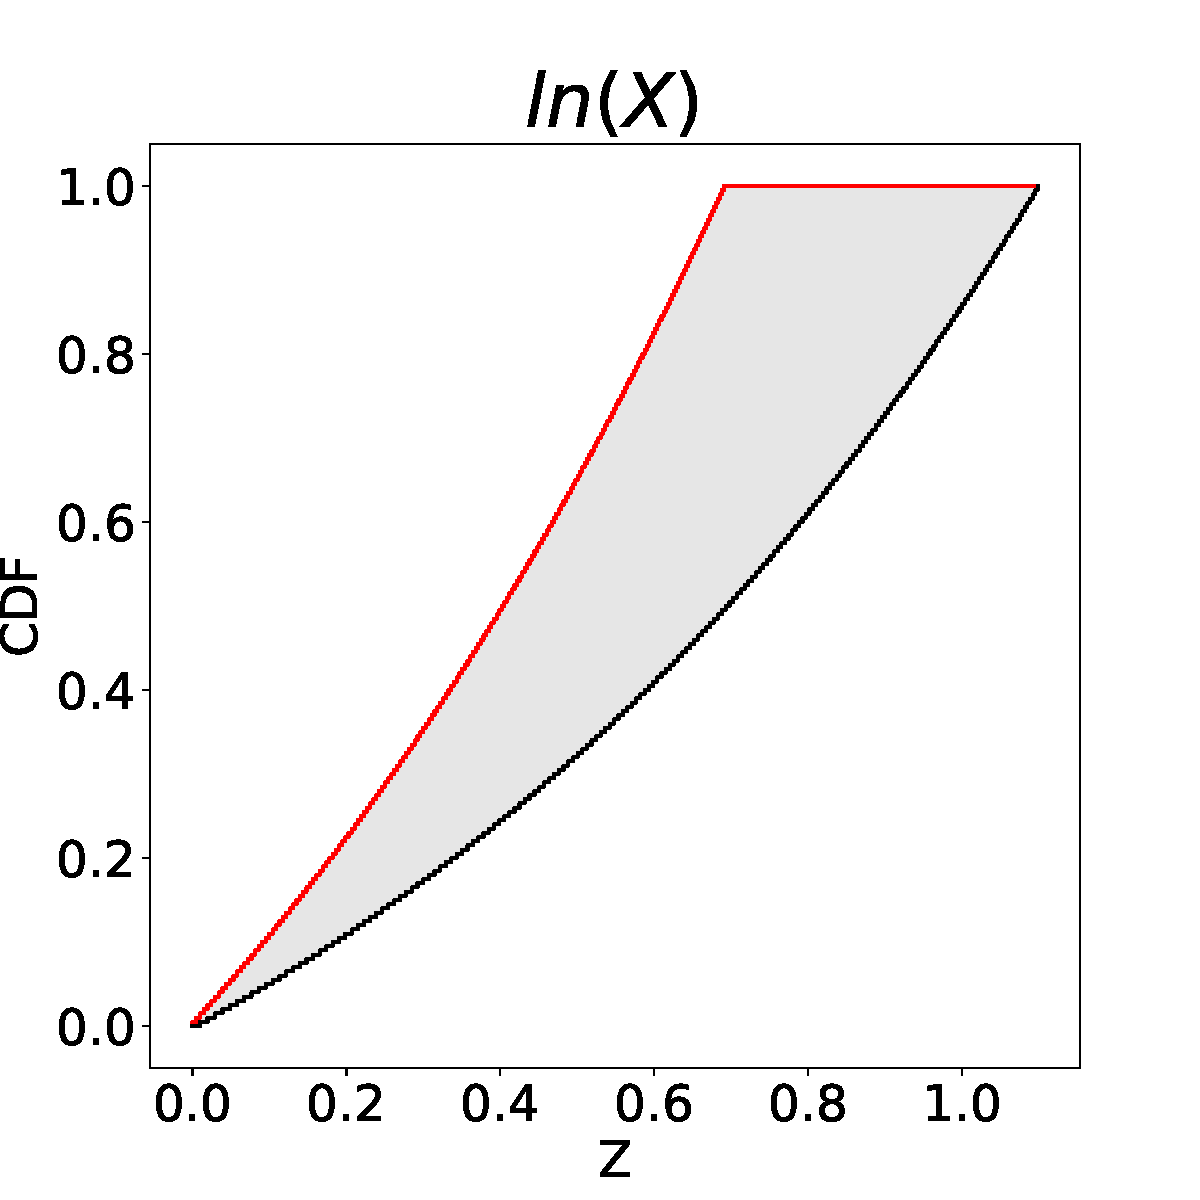
\includegraphics[width=.25\textwidth]{../examples/JuliaCon/fig8/fig8_pbox5.pdf}\hfill
  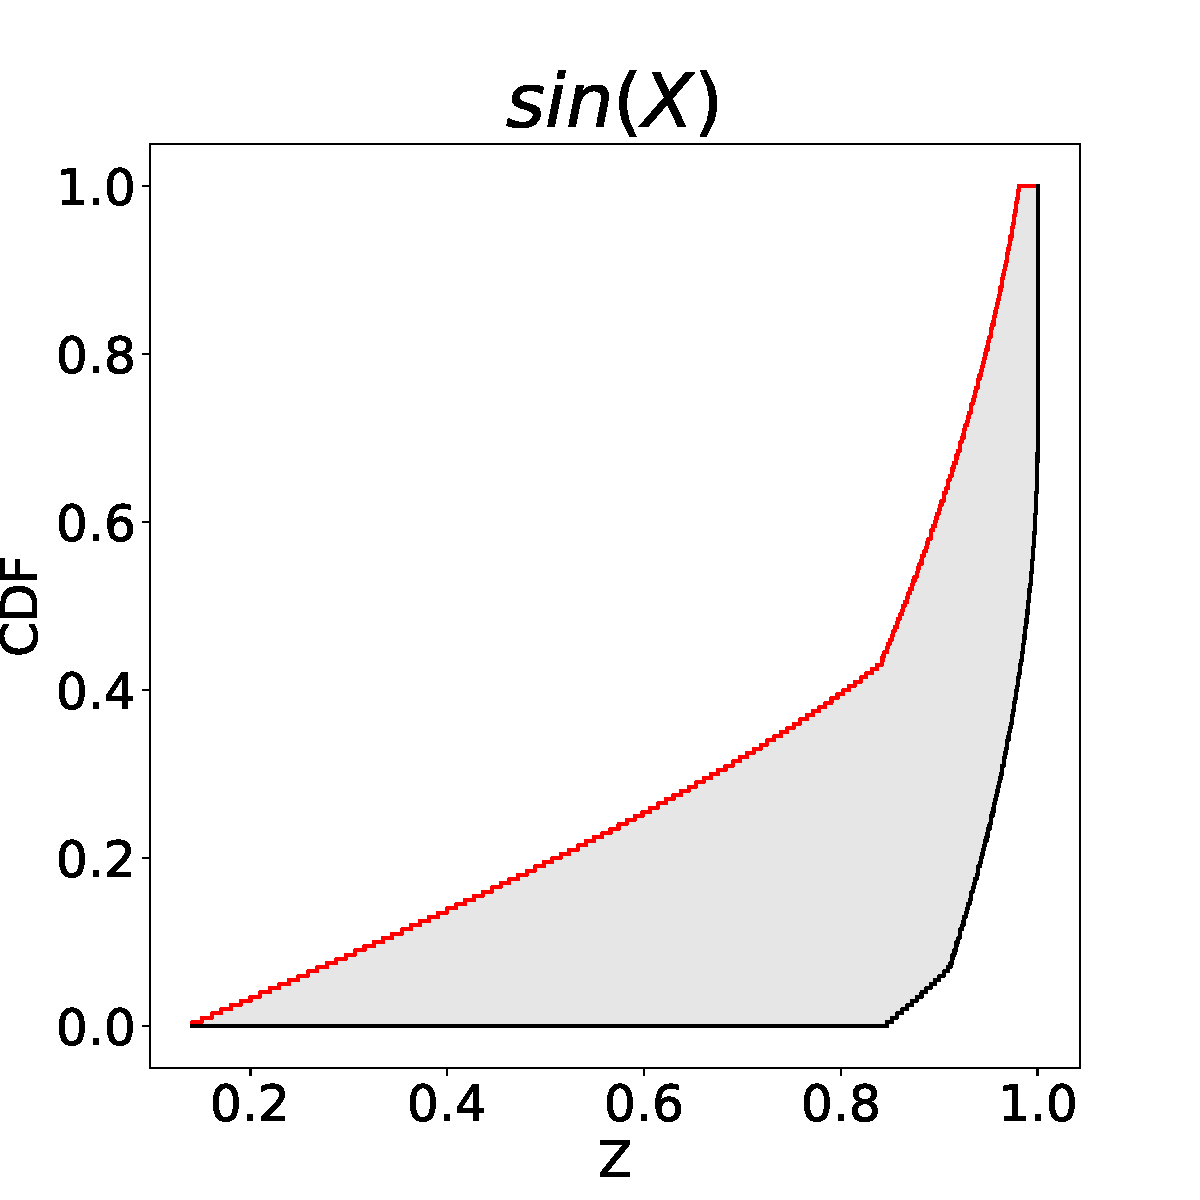
\includegraphics[width=.25\textwidth]{../examples/JuliaCon/fig8/fig8_pbox6.pdf}\hfill
  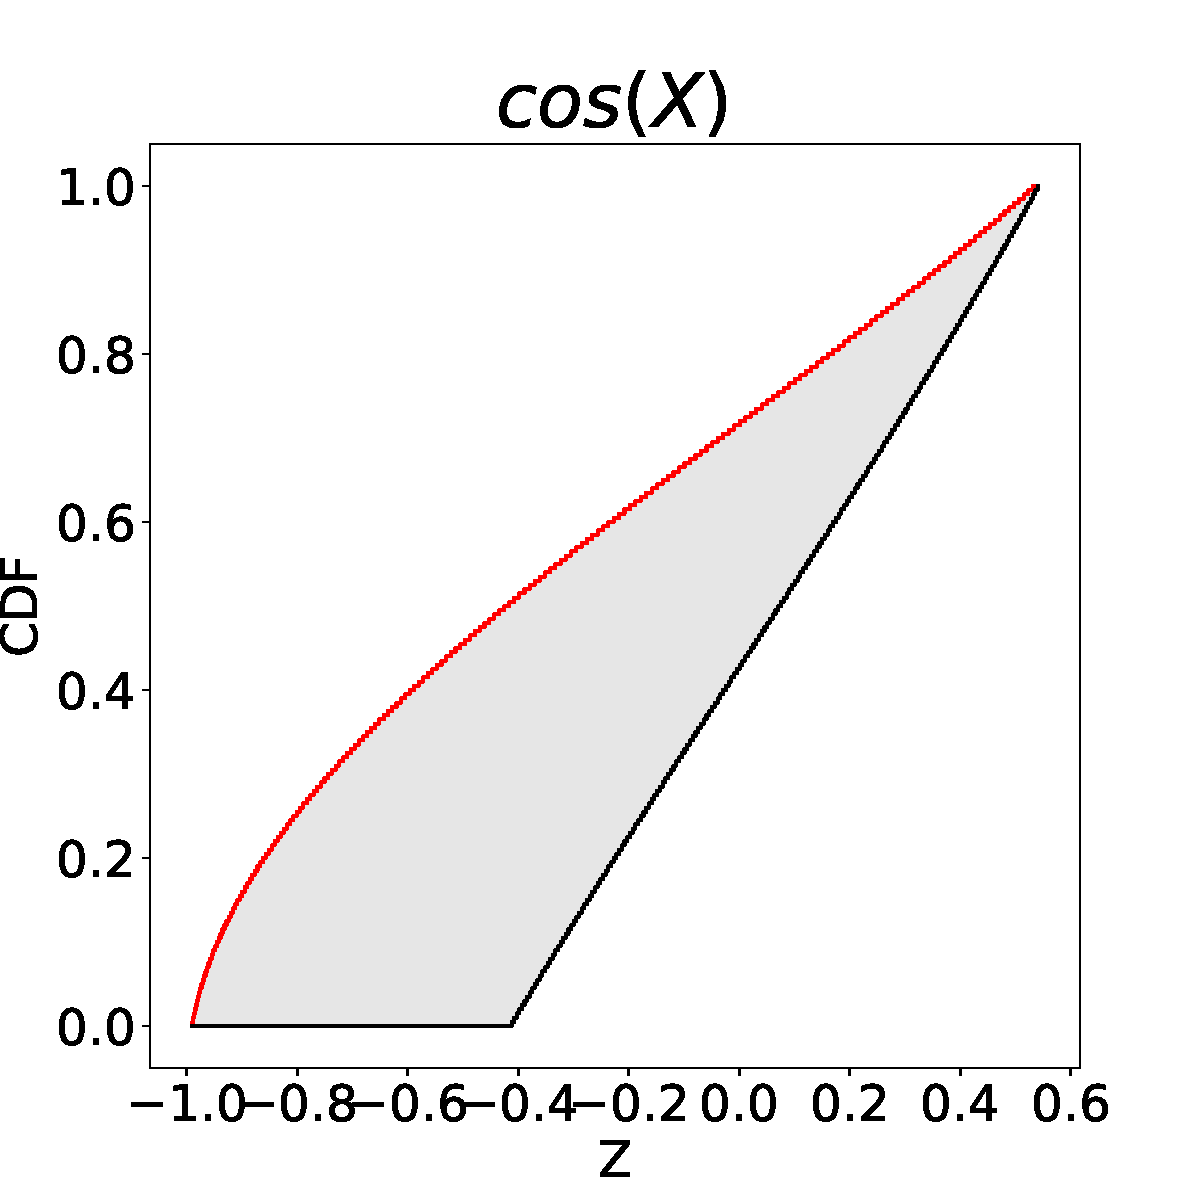
\includegraphics[width=.25\textwidth]{../examples/JuliaCon/fig8/fig8_pbox7.pdf}\hfill
  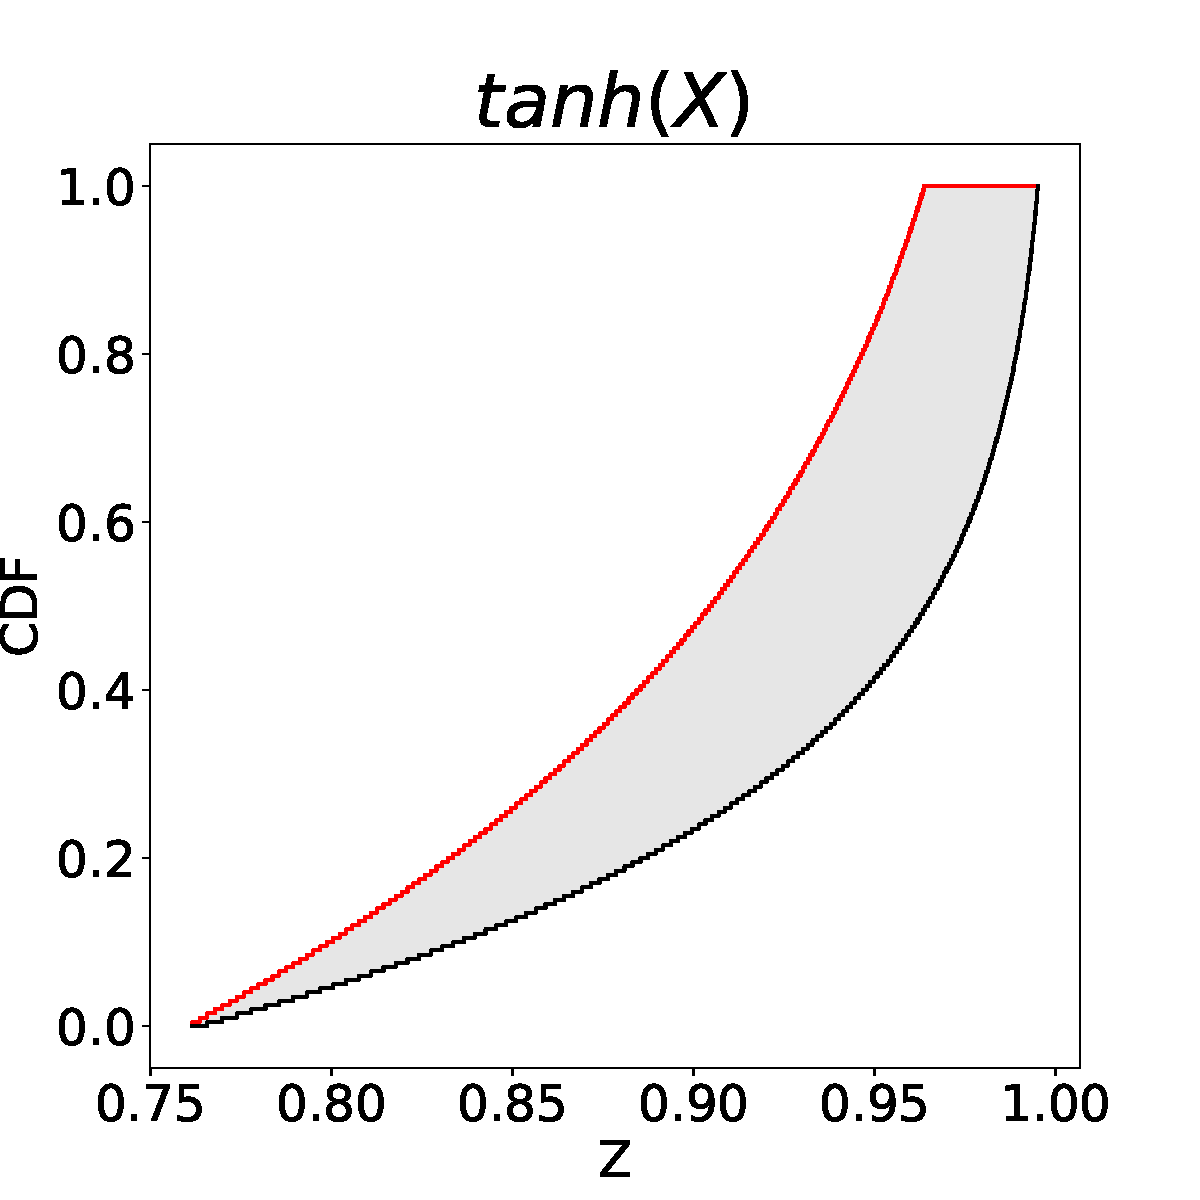
\includegraphics[width=.25\textwidth]{../examples/JuliaCon/fig8/fig8_pbox8.pdf}
  

  \caption{Top left shows an initial p-box, and others show results of unary operations on this p-box}
  \label{fig:figure8}
  
\end{figure*}

\section{P-box arithmetic}
\label{sec:pboxarithmetic}

In this section we will discuss how p-boxes can be propagated through unary and binary operations in a rigorous way.

\subsection{Unary operations}
Piggybacking off \texttt{IntervalArithmetic.jl}\footnote{https://github.com/JuliaIntervals/IntervalArithmetic.jl} \cite{david_p_sanders_2021_5519761}, a p-box can be transformed through any unary operation $f: \mathbb{R} \rightarrow \mathbb{R}$ that has  an interval extension, i.e. accepts intervals. For this, we first transform the p-box into a Dempster-Shafer structure \cite{dempster2008upper,shafer1976mathematical}, propagate the structure through the operation with interval arithmetic, and transform it back to a p-box. A Dempster-Shafer structure (also called a belief function) is a finite collection of intervals, called focal elements $X$, with probabilities attached to each interval, called basic mass assignments $m$, which must sum to $1$. An example of a belief function with three focal elements is: $X = \{[0, 2], [0.5, 1.3], [1, 3]\}$ and $m = \{0.25, 0.5, 0.25\}$. Like a p-box, a Dempster-Shafer also bounds a set of probability distributions, using two set based functions called the \textit{belief} and \textit{plausibility}:

\begin{align*}
  \text{bel}(U) &= \sum_{X \subseteq U} m(X),\\ 
  \text{pl}(U) &= \sum_{X \cap U \neq \emptyset} m(X),
\end{align*}

where the sum is taken over focal elements $X$. For example, the belief and plausibility of $U = [0,2.5]$ are $\text{bel}([0,2.5]) = 0.75$ (\{$[0, 2]$, $[0.5, 1.3]$\} are subsets) and $\text{pl}([0, 2.5]) = 1$ (all focal elements intersect). The belief and plausibility serve as lower and upper bounds on the probability measure:

\begin{equation*}
  \text{bel}(U) \leq \mathbb{P}(U) \leq \text{pl}(U) .
\end{equation*}


A p-box is a special case of a belief function, where the focal elements are ordered by $\leq$. Looking at the leftmost p-box in Figure \ref{fig:figure2} (with $4$ steps) it can be seen that the p-box could be represented with $4$ intervals (i.e. each box in the plot is a focal element). The mass assignment
in this case is the difference in cdf level of each box $p_{i+1} - p_{i}$, which gives an equal mass assignment since we discretised the p-box uniformly. Note that for a general belief function, the focal elements do not have to be ordered, as is in the case of the previous example: $X = \{[0, 2], [0.5, 1.3], [1, 3]\}$. The following function converts a p-box into a belief function:

\begin{lstlisting}[language = Julia]
  function split(F :: pbox)

    n = length(F.u)

    focal_el = interval.(F.u, F.d)
    masses   = ones(n) ./n

    return focal_el, masses
  end
\end{lstlisting}

A belief function can be converted to a p-box by accumulating the belief and plausibility (the lower and upper probability):

\begin{align*}
  \underline{F}(x) &= \text{bel}((-\infty, x]),\\ 
  \overline{F}(x) &= \text{pl}((-\infty, x]),
\end{align*}

which numerically corresponds to sorting the bounds of the focal elements, accumulating the basic mass assignments, and finding the probability levels. Assuming that the basic mass assignments are equal, the following code converts a belief function into a p-box:

\begin{lstlisting}[language = Julia]
  function makepbox(focal_el)

    x_lo = getfield.(focal_el, :lo);
    x_hi = getfield.(focal_el, :hi);

    u = sort(x_lo)
    d = sort(x_hi)

    return pbox(u, d)
  end
\end{lstlisting}

The general function where the focal elements have non-equal mass is simple, but slightly lengthy, and will not be described here. A function to perform a unary operation on a p-box is thus:

\begin{lstlisting}[language = Julia]
  function unary(F :: pbox, op)

    focal_el, _ = split(F)
    fe_z = op.(focal_el)

    return makepbox(fe_z)
  end
\end{lstlisting}

Figure \ref{fig:figure8} show examples of unary operations on a p-box.

\subsection{Binary operations}
\label{sec:pboxBinary}
Binary operations on p-boxes are based on \textit{convolutions}, which are operations on two functions which produce a third. A convolution often used in signal processing is: 

\begin{equation*}
  f_{Z}(z) = \int^{\infty}_{-\infty}f_{X}(z-x)f_{Y}(x)dx .
\end{equation*}

It is well known that the result of above convolution $f_{Z}$ corresponds to the probability density of the sum of two independent random variables with densities $f_{X}$ and $f_{Y}$. P-box arithmetic is based on generalisations of such convolutions specifically designed for computing binary operations on distribution functions, which work with operations other than sum, and for copulas other than independence. These convolutions, which first appeared in the study of Probabilistic Metric Spaces \cite{schweizer2011probabilistic}, can be be used to compute binary operations between two p-boxes when their copula $C$ is precisely known, only it's lower bound is known $\underline{C}$, or even missing completely. Further, Williamson and Downs \cite{williamson1990probabilistic} describe how robust outer approximations of the convolutions can be found, accounting for the representation error of the two input p-boxes, as well as the error from the integration.

\subsubsection{Operations with known $C$} \hfill \break

\begin{figure*}[htp]

  \centering
  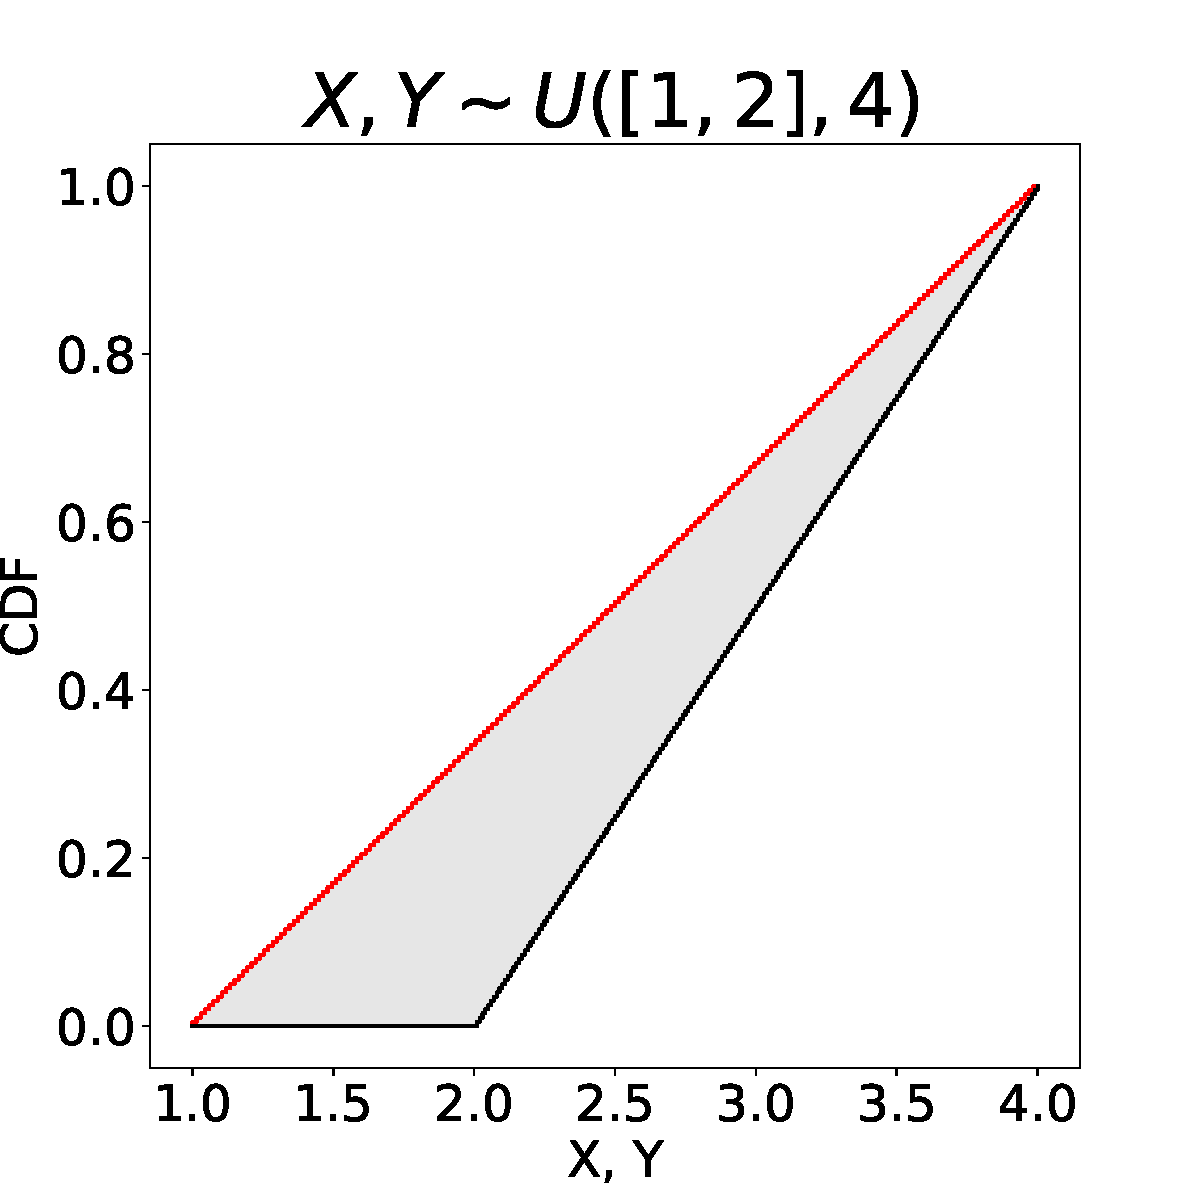
\includegraphics[width=.25\textwidth]{../examples/JuliaCon/fig9/fig9_pbox1.pdf}\hfill
  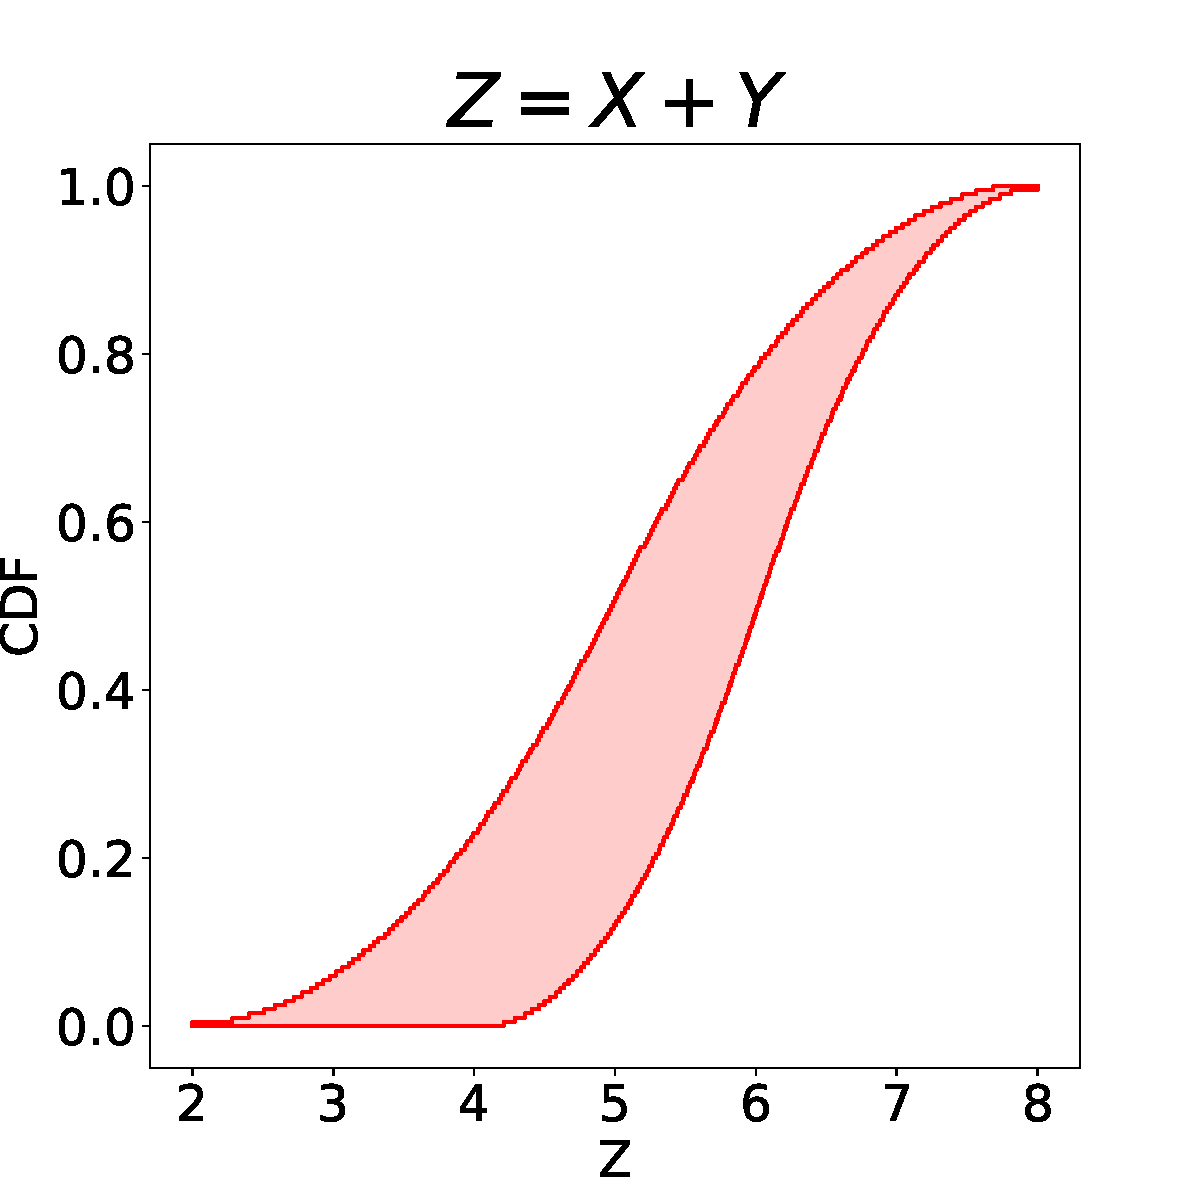
\includegraphics[width=.25\textwidth]{../examples/JuliaCon/fig9/fig9_pbox2.pdf}\hfill
  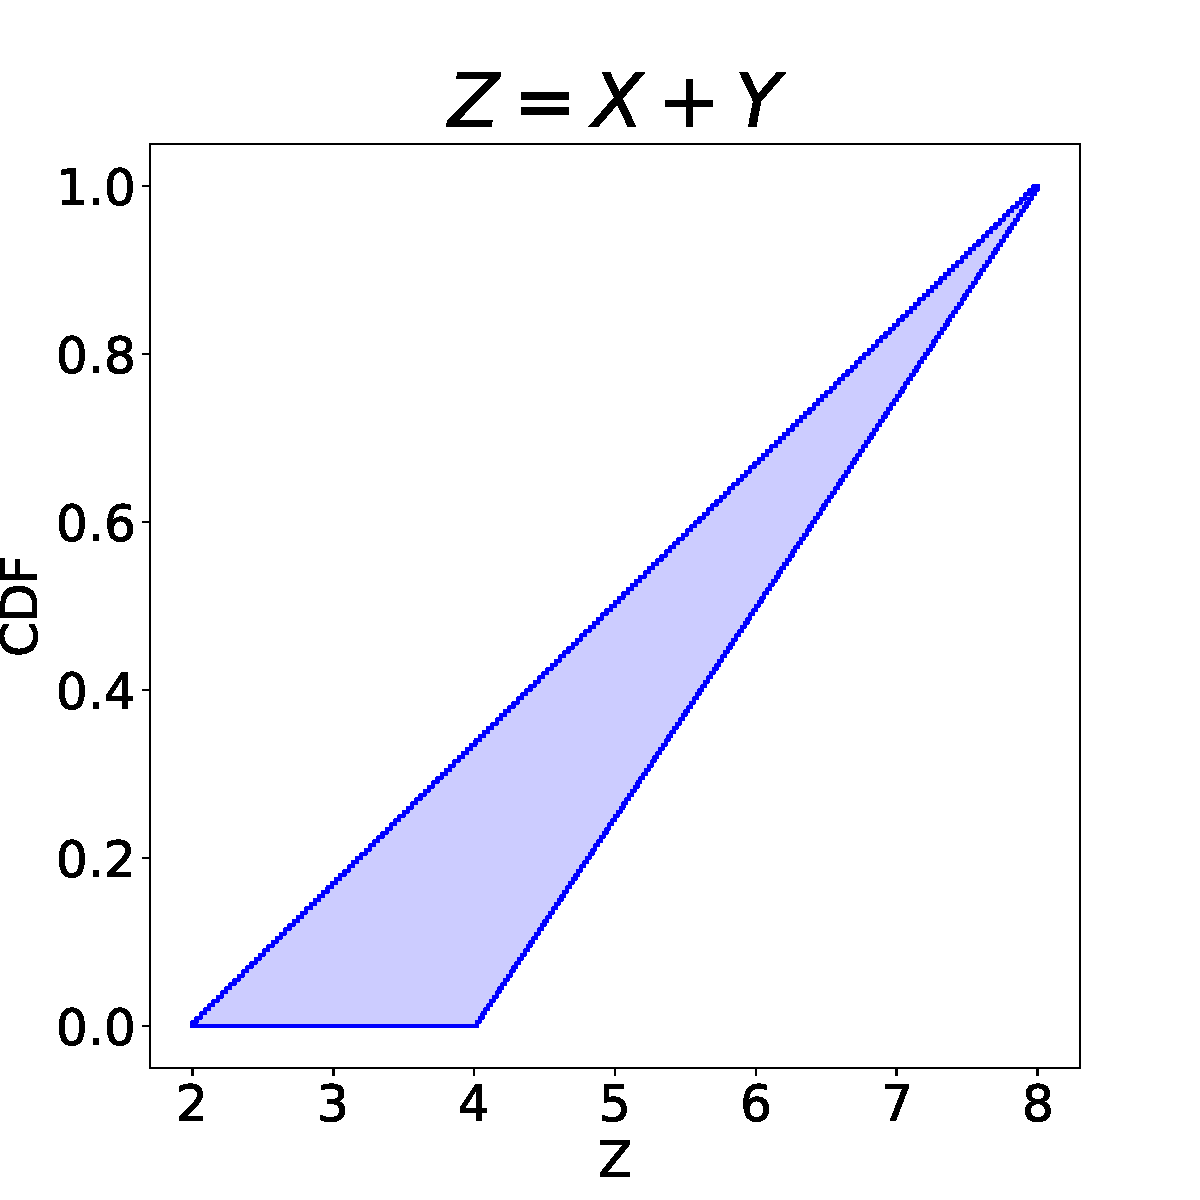
\includegraphics[width=.25\textwidth]{../examples/JuliaCon/fig9/fig9_pbox3.pdf}\hfill
  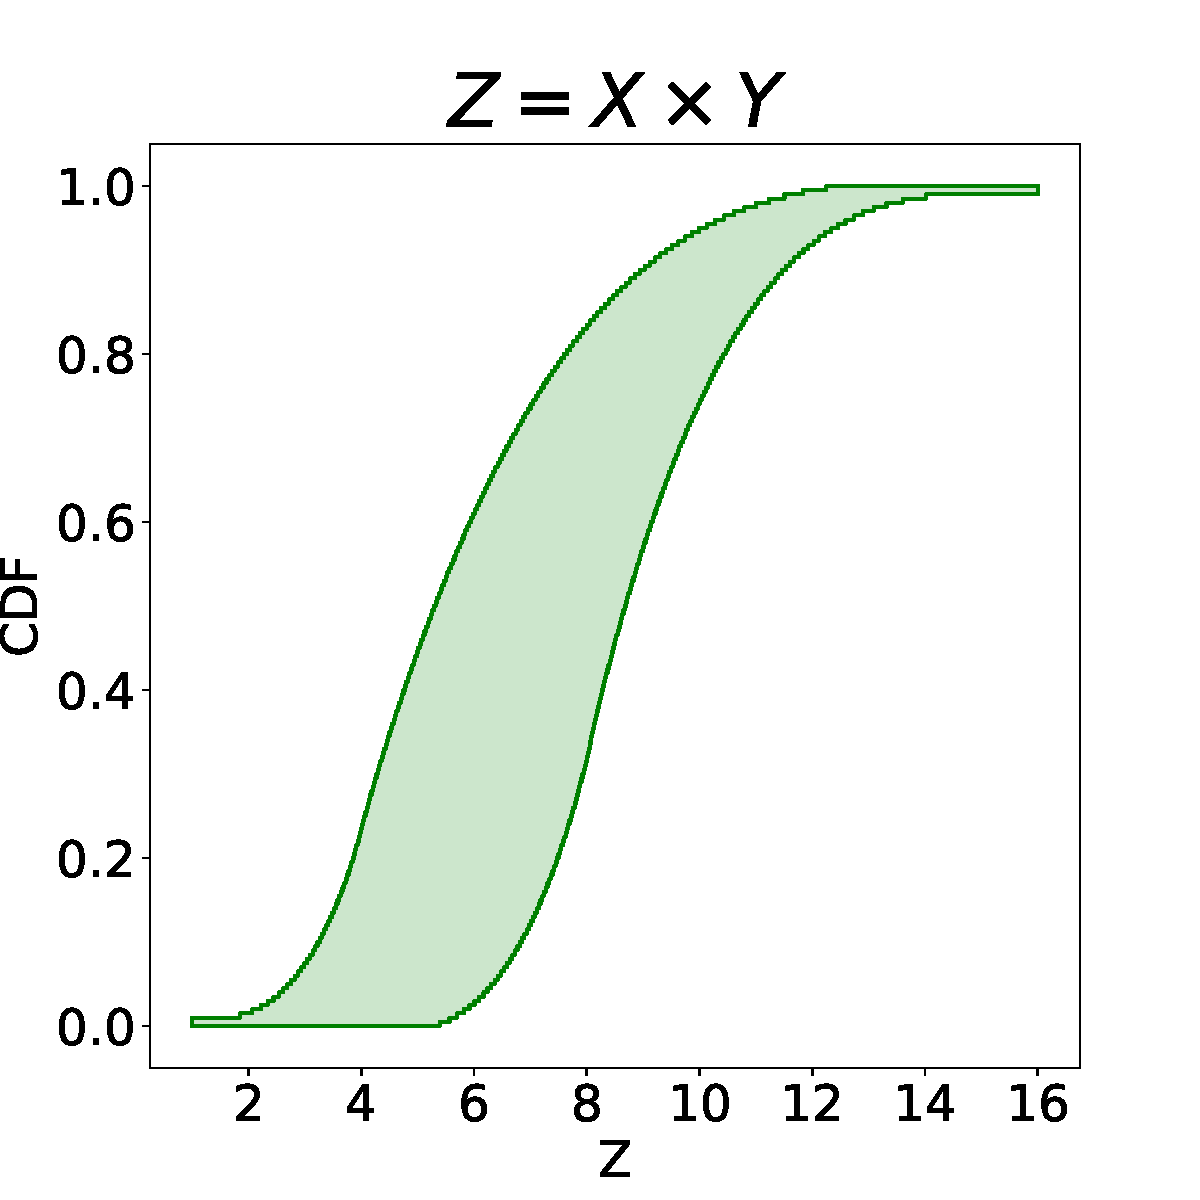
\includegraphics[width=.25\textwidth]{../examples/JuliaCon/fig9/fig9_pbox4.pdf}
  

  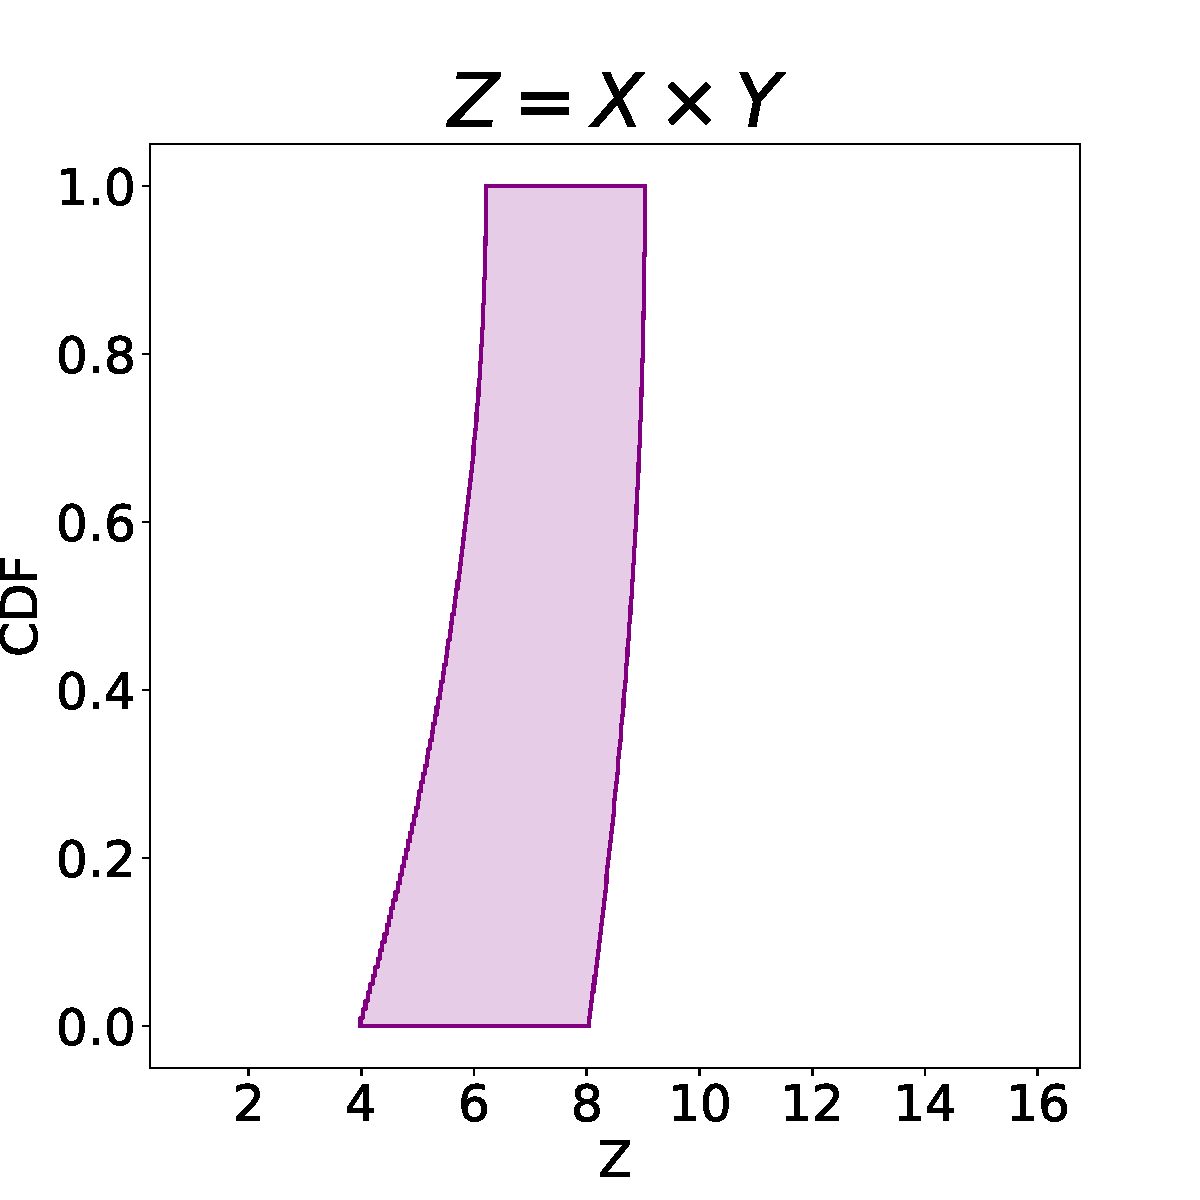
\includegraphics[width=.25\textwidth]{../examples/JuliaCon/fig9/fig9_pbox5.pdf}\hfill
  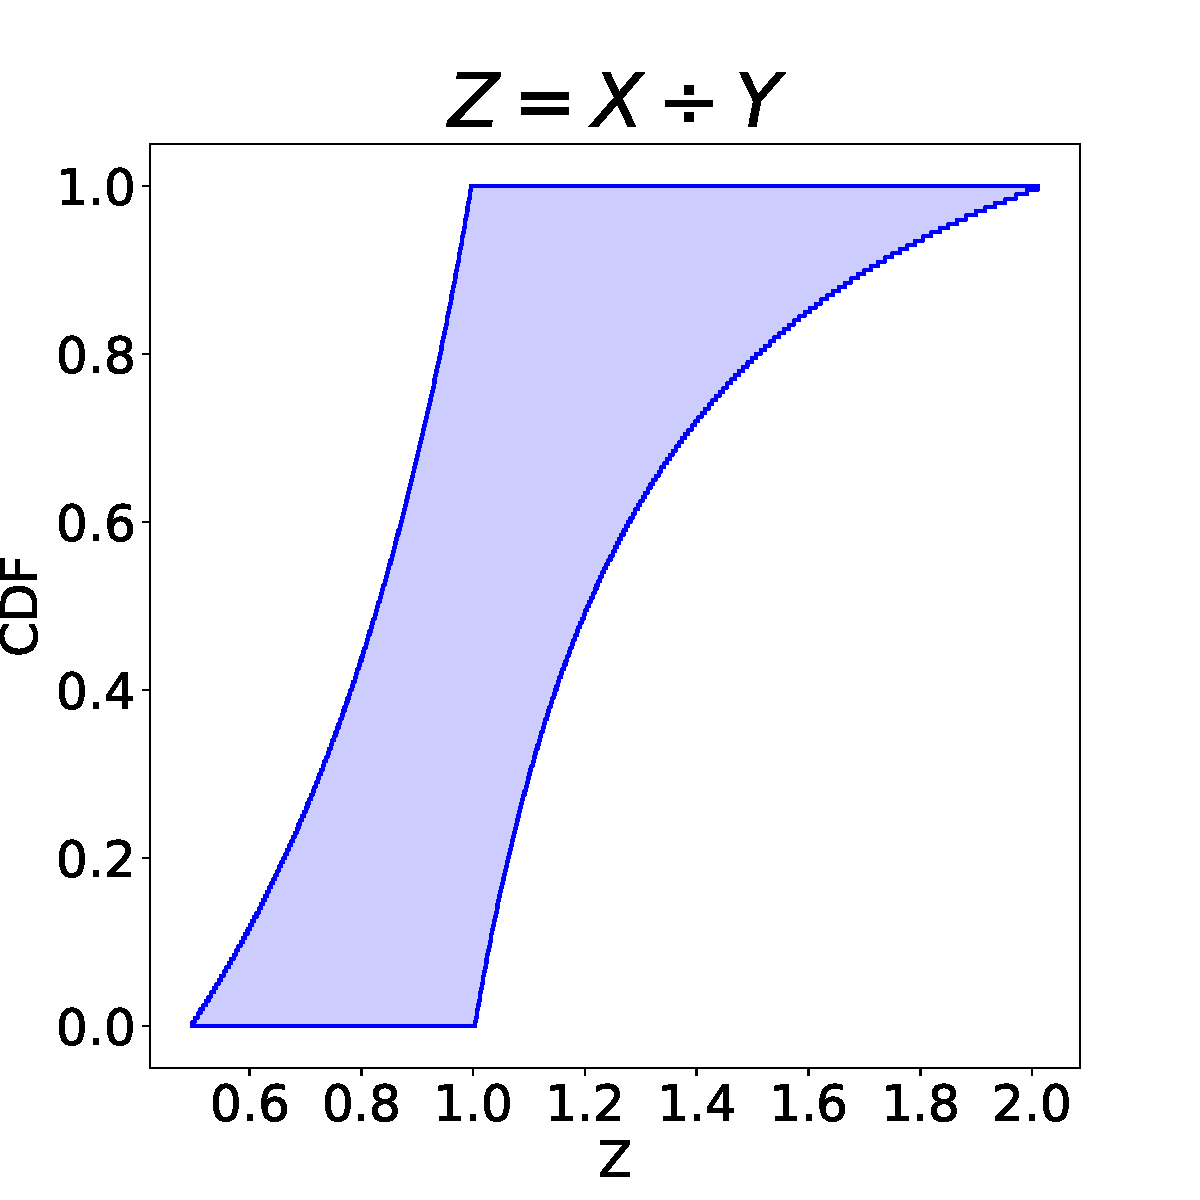
\includegraphics[width=.25\textwidth]{../examples/JuliaCon/fig9/fig9_pbox6.pdf}\hfill
  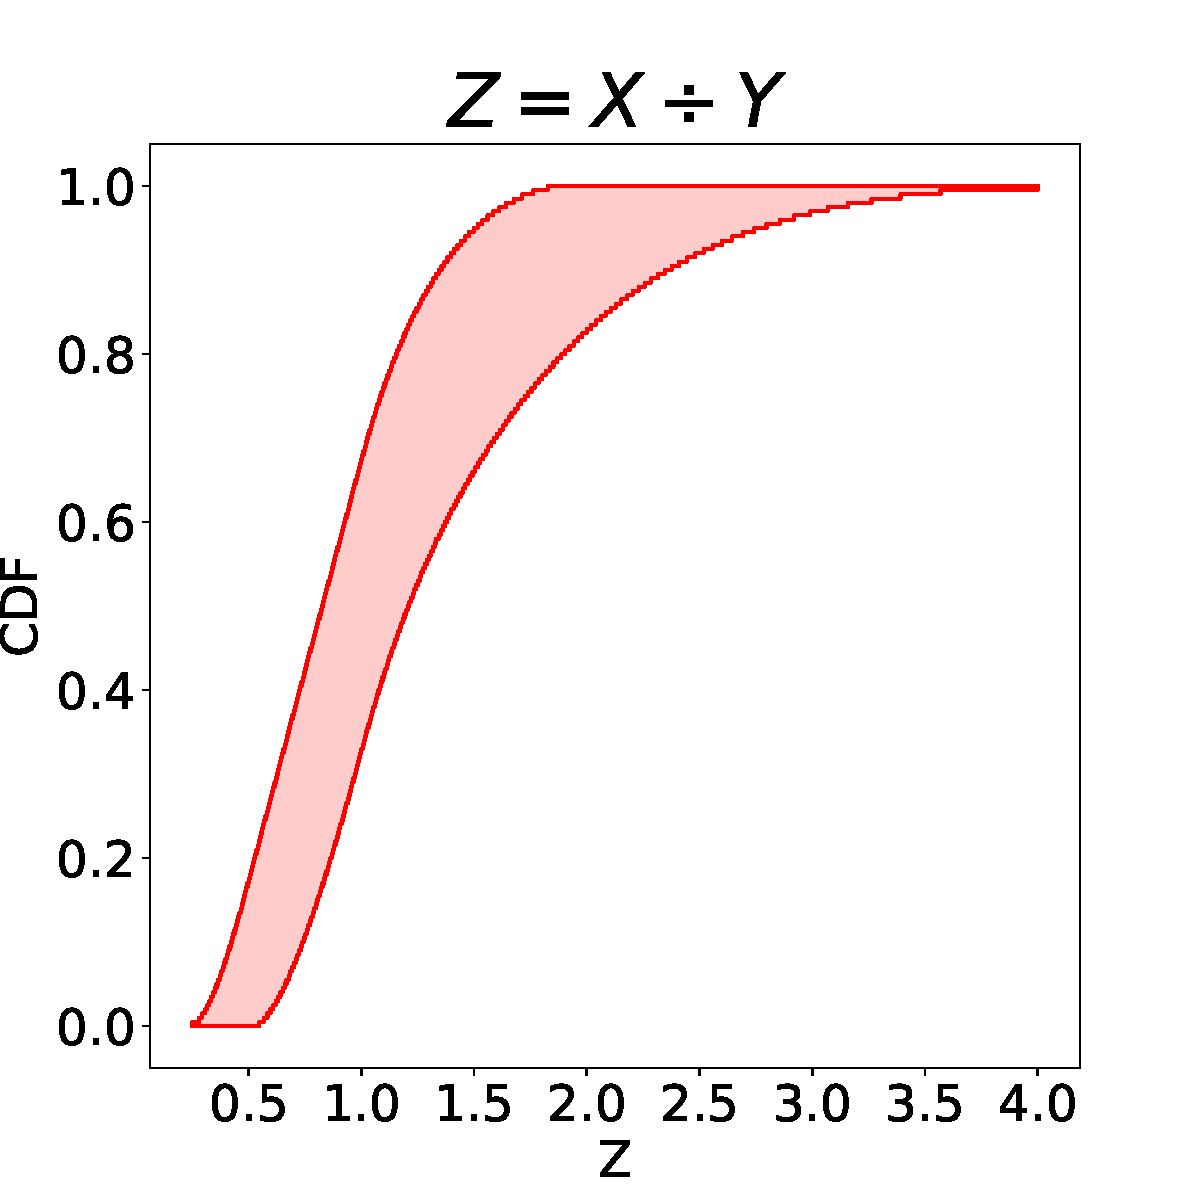
\includegraphics[width=.25\textwidth]{../examples/JuliaCon/fig9/fig9_pbox7.pdf}\hfill
  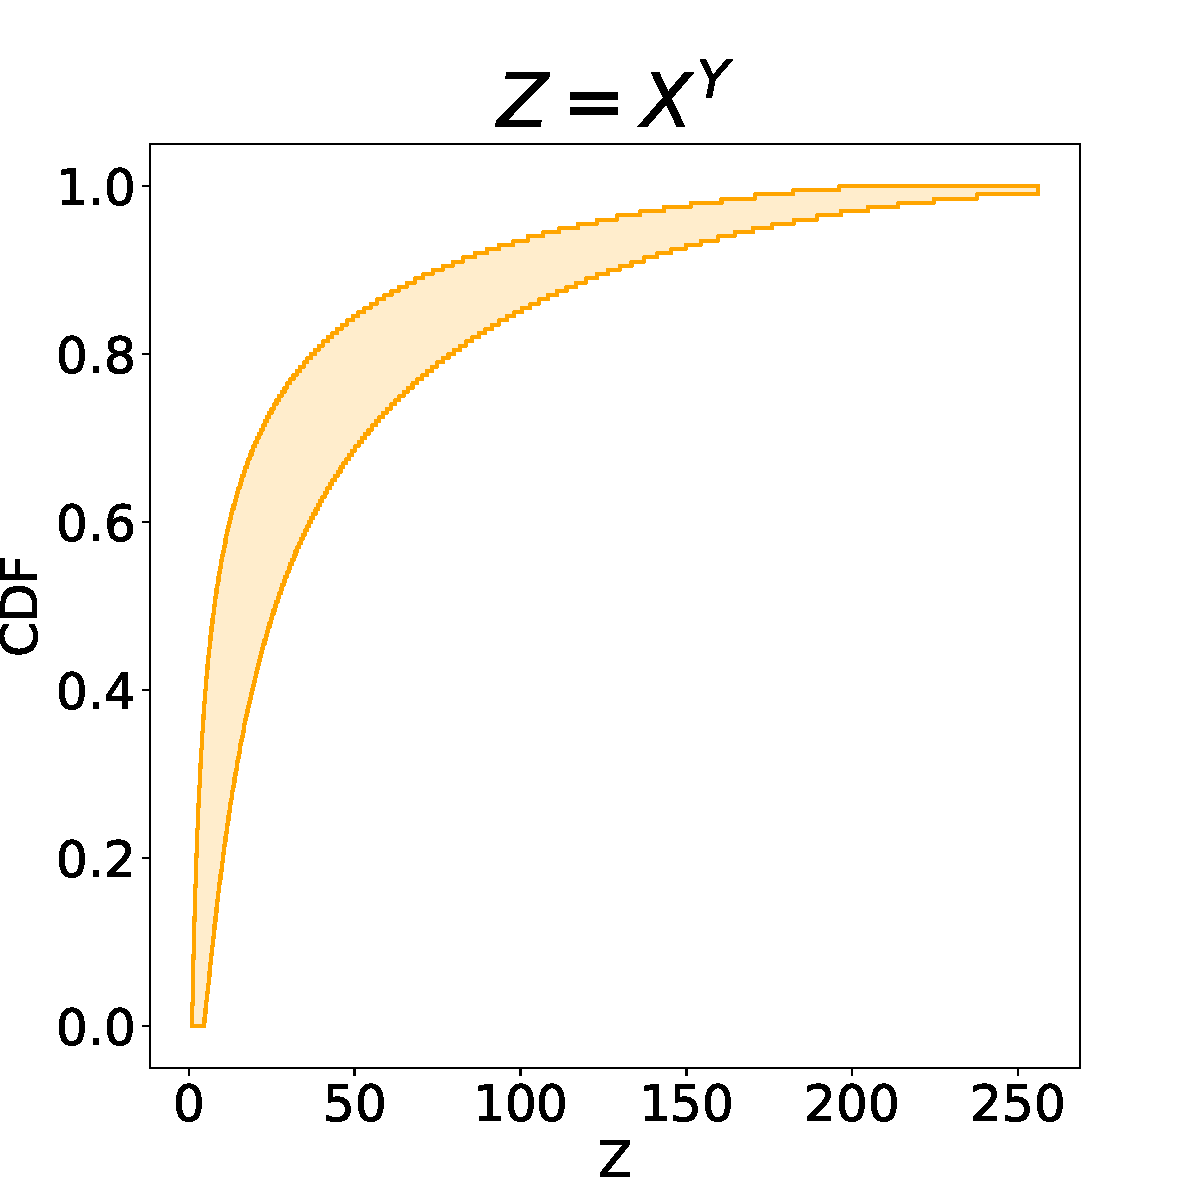
\includegraphics[width=.25\textwidth]{../examples/JuliaCon/fig9/fig9_pbox8.pdf}
  

  \caption{Top left shows two initial p-boxes $X, Y \sim U([1,2], 4)$, and others show results of binary operations on these two p-boxes with different dependencies. Each colour represents a different copula. The colour code is $C = \{$ {\color{purple} $W$} (opposite), {\color{green} $\Phi_{-0.5}$ }(correlation -0.5), {\color{red} $\Pi$} (independence), {\color{orange} $\Phi_{0.5}$} (correlation 0.5), {\color{blue} $M$}(perfect) $\}$}
  \label{fig:figure9}
  
\end{figure*}


A binary operation between two random variables $X$ and $Y$ with cdfs $F_{X}$ and $F_{Y}$ and copula $C$ can be computed with the following Lebesgue-Stieltjes integral: 

\begin{equation*}
  \sigma_{C,L}(z) = \int_{L\{z\}}dC(F_{X}(x),F_{Y}(y)) ,
\end{equation*}

where the integration domain is the set $L\{z\} = \{(x,y)| x,y \in \mathbb{R}, L(x,y) < x\}$ (the set of all $x$ and $y$ for which $L(x,y) < z$), and where $L$ is some binary operation (e.g. $L(x,y) = x+y$). The above $\sigma_{C,L}$ convolution is written for precise distributions, however can be extended for p-boxes by performing the convolution with some combination of the p-boxes bounds in the style of interval arithmetic:


\begin{eqnarray*}
  + 
  \begin{cases}
    \underline{F_Z} = \underline{F_X} + \underline{F_Y} \vspace{2mm}\\
    \overline{F_Z} = \overline{F_X} + \overline{F_Y}
  \end{cases}
  \\
  -\begin{cases}
    \underline{F_Z} = \underline{F_X} - \overline{F_Y}\vspace{2mm}\\
    \overline{F_Z} = \overline{F_X} - \underline{F_Y}
  \end{cases}
  \\
  \times
  \begin{cases}
    \underline{F_Z} = \underline{F_X} \times \underline{F_Y}\vspace{2mm}\\
    \overline{F_Z} = \overline{F_X} \times \overline{F_Y}
  \end{cases}
  \\
  \div
  \begin{cases}
    \underline{F_Z} = \underline{F_X} \div \overline{F_Y}\vspace{2mm}\\
    \overline{F_Z} = \overline{F_X} \div \underline{F_Y}
  \end{cases}
\end{eqnarray*}

Williamson and Downs provide an algorithm to compute rigorous bounds on the above convolution, but only under independence (when $C = \Pi$). Around the same time, Yager \cite{yager1986arithmetic} described a similar style convolution on two belief functions under the assumption independence, which is very similar to that of Williamson and Downs'. We therefore provide a generalised version of Yager's algorithm where any copula $C$ can be specified. Similar to a unary operation, a binary operation between two p-boxes can be performed by first transforming the bivariate p-box into a two dimensional belief function (which has interval boxes as focal elements), evaluating the operation on the focal elements with interval arithmetic, and transforming the resulting belief function (which will be univariate after the operation) back to a p-box. Converting a bivariate p-box into a 2D belief function is similar to that of the 1D case, however this time the mass assignment $m$ will be determined by the copula $C$. For two univariate focal elements $X$ and $Y$ with probability widths $p_{x} = [p_{x1}, p_{x2}]$ and $p_{y} = [p_{y1}, p_{y2}]$ (i.e. their vertical width in Figure \ref{fig:figure2}, with their 1D mass assignment being $p_{x2} - p_{x1}$), the 2D mass assignment of the interval box $X \times Y$ will be: 

\begin{equation*}
  C(p_{x2}, p_{y2}) - C(p_{x1}, p_{y2}) - C(p_{x2}, p_{y1}) + C(p_{x1}, p_{y1}) .
\end{equation*}

The following function converts a bivariate p-box into a 2D belief function: 

\begin{lstlisting}[language = Julia]
  function split(F :: BivPbox)

    X = F.X; Y = F.Y; C = F.C
    
    nx = length(X.u); ny = length(Y.u);

    px = range(0, 1, length = nx + 1);
    py = range(0, 1, length = ny + 1);

    f_el_X = interval.(X.u, X.d);
    f_el_Y = interval.(Y.u, Y.d);
    
    masses = C(px[2:end],   py[2:end]) 
           - C(px[1:end-1], py[2:end]) 
           - C(px[2:end],   py[1:end-1]) 
           + C(px[1:end-1], py[1:end-1]);

    f_XY   = [IntervalBox(x,y) for x in f_el_X, 
                                   y in f_el_Y];

    return f_XY[:], masses[:]
  end
\end{lstlisting}

A robust $\sigma$ convolution is simply thus: 

\begin{lstlisting}[language = Julia]
  function sigma(F :: BivPbox, op)

    nx = length(F.X.u); ny = length(F.Y.d);

    # number of steps of output
    num_steps = max(nx, ny);
    
    # Convert pbox to a belief function
    fe, masses = split(F)

    # Perform operation with interval arithmetic
    fe_z = [op(f.v[1],f.v[2]) for f in fe]
    
    # Convert back to p-box
    return makepbox(fe_z, masses, num_steps)
  end
\end{lstlisting}

The above $\sigma$ convolution will work for any two input p-boxes, with any copula $C$, and binary operation $op$ which has an interval extension. Again the general function for converting a belief function with non-equal masses is required. The 3rd argument \textit{num\_steps} is the desired discretisation of the output p-box, in a condensation step. The interval operation in the $\sigma$ convolution performs the operation on all combinations of focal elements, so for example if each p-box has 200 steps, the resulting p-box will have $200 \times 200 = 40,000$ steps, which must be reduced in an outer approximation. Again, the general algorithm is simple but lengthy and will be omitted. Figure \ref{fig:figure9} shows examples of $\sigma$ convolutions for different operators and copulas.

\subsubsection{Operations with lower bound $\underline{C}$} \hfill \break

\texttt{ProbabilityBoundsAnalysis.jl} also allows for binary operations to be performed between p-boxes when only the lower bound of the copula is known $\underline{C}$. That is, uncertainty can be placed on the dependence of two distributions, as well as the marginals. The resulting p-box of the binary operation will bound all distributions with copulas $C$ which are pointwise greater than the specified copula $\underline{C} \leq C$. These operations are based on two more convolutions from Probabilistic Metric Spaces \cite{schweizer2011probabilistic}. For a non-decreasing binary operator $L: \mathbb{R}^+\times \mathbb{R}^+ \to \mathbb{R}^+$, two random variables $X$ and $Y$ with distribution functions $F_X$ and $F_Y$, and with copula lower bound $\underline{C}$:

\begin{equation*}\label{taupbox}
  \tau_{\underline{C}_{XY},L}(z) = \sup_{L(x,y)=z} [\underline{C}(F_{X}(x), F_Y(y))],
\end{equation*}
\begin{equation*}\label{rhopbox}
  \rho_{\underline{C}_{XY},L}(z) = \inf_{L(x,y)=z} [\underline{C}^d(F_{X}(x), F_Y(y))],
\end{equation*}

where $C^d$ is the copula dual of $C$, $C^d(u,v) = u + v - C(u,v)$. The $\tau$ and $\rho$ convolutions each compute a cdf bound which together characterise the resulting p-box: $[\underline{F}_{Z}(z), \overline{F}_{Z}(z)] = [\tau(z), \rho(z)]$. The p-box resulting from a $\tau$ and $\rho$ convolution will bound all $\sigma$ convolutions which have copula $C$ which is greater than $\underline{C}$. For example, setting $\underline{C} = W$ (the lower bound on all copulas) will propagate all copulas, which is complete uncertainty about the dependence, i.e. a \textit{Fréchet} operation. Setting $\underline{C} = \Pi$ will propagate copulas more positive than independence, otherwise known as \textit{positive quadrant dependence} \cite{nelsen2007introduction}. Setting $\underline{C} = M$ (the upper bound on all copulas) will only propagate $M$, and will be equal to a $\sigma$ convolution. 

The $\tau$ and $\rho$ convolutions can be efficiently computed in terms of the inverse representation using in \textit{ProbabilityBoundsAnalysis}: 

\begin{equation*}\label{taupbox2}
  \tau^{-1}_{\underline{C}_{XY},L}(p) = \sup_{\underline{C}(u,v) = p} [L(F^{-1}_{X}(u), F^{-1}_Y(v))],
\end{equation*}
\begin{equation*}\label{rhopbox2}
  \rho^{-1}_{\underline{C}_{XY},L}(p) = \inf_{\underline{C}^{d}(u,v) = p} [L(F^{-1}_{X}(u), F^{-1}_Y(v))],
\end{equation*}

where the operation $L$ is performed on the $u$ and $d$ vectors of the p-boxes, and $\sup_{\underline{C}(u,v) = p}$ and $\inf_{\underline{C}^{d}(u,v) = p}$ is solved for each probability level.

Note that $L$ must be non-decreasing function (for example $+$ or $\times$), but may be extended to non-increasing functions (for example $-$ or $\div$) by first transforming one of the variables, and performing a non-decreasing operation. For example, $X - Y$ can be evaluated with sum: $X + (-Y)$. Note however, the copula $C_{XY}$ must also be transformed to $C_{X,-Y}$. This transformation however is quite simple \cite{nelsen2007introduction}: 

\begin{equation*}\label{rotation}
  C_{X, -Y}(u,v) = u - C_{XY}(u, 1 - v).
\end{equation*}

Note that when using the above copula transformation, the bound on $\underline{C}_{XY}$ will be flipped to $\overline{C}_{X, -Y}$, and $\tau_{M, -}$ and $\rho_{M,-}$ give the \textit{Fréchet} convolution.

\iffalse
\section{An uncertain programming language}
\label{sec:additional_faci}

The long term goal of such a framework is to create a fully uncertain programming language, where any computer variable may be represented as an interval, distribution, p-box or other uncertain quantity. Such a framework would allow for uncertain extensions of deterministic functions to be computed in an automatic, rigorous and tight fashion. In this section we argue why Julia is an ideal target language for such a framework, and discuss some of the remaining theoretical tasks required to make such a goal a reality. 
\fi

\section*{Acknowledgements}
We would like to thank our friends and colleagues at the Risk Institute who have supported \texttt{ProbabilityBoundsAnalysis.jl} from its birth, and through their contributions and discussions have made this software possible: Marco De Angelis, Nick Gray, Alex Wimbush and Dominic Calleja. We also thank Dominic and Liam Henry's (Clarus Financial Technology, Belfast) detailed review of this paper.

We are also specially grateful to the researchers at JuliaReach and JuliaIntervals, who through their interest, contributions, discussions and suggestions have greatly improved the software: Marcello Forets, Christian Schilling, Luis Benet and David P. Sanders.

The authors would like to thank the support of this work from the Engineering Physical Sciences Research Council (EPSRC) iCase studentship award. This research is funded by the EPSRC with grant number EP/R006768/1, which is acknowledged for its funding and support. This work has been carried out within the frame- work of the EUROfusion Consortium and has received funding from the Euratom research and training programme 2014–2018 and 2019–2020 under grant agreement number 633053. The views and opinions expressed herein do not necessarily reflect those of the European Commission.

% **************GENERATED FILE, DO NOT EDIT**************

\bibliographystyle{juliacon}
\bibliography{ref.bib}


\end{document}

% Inspired by the International Journal of Computer Applications template
